\documentclass[a4paper, 12pt]{report}
\usepackage[T1]{fontenc}
\sloppy 
\usepackage[a4paper, left=2.5cm, right=2.5cm, top=3cm, bottom=3cm]{geometry}
\usepackage{color}
\usepackage{times}
\usepackage{booktabs}
\usepackage{afterpage}
\usepackage[utf8]{inputenc}
\usepackage[spanish]{babel}
\usepackage{url}
\usepackage{graphicx}
\usepackage{subfigure}
\usepackage{float}  %% H para posicionar figuras
\usepackage[nottoc, notlot, notlof, notindex]{tocbibind} %% Opciones de índice
\usepackage[none]{hyphenat}
\usepackage{cite}
\usepackage[bookmarks = true, colorlinks=true, linkcolor = black, citecolor = black, menucolor = black, urlcolor = blue]{hyperref}
\setcounter{tocdepth}{3}
\setcounter{secnumdepth}{3}
\usepackage{listings}
\usepackage{makecell}

\begin{document}
	\pagestyle{empty}
	\begin{titlepage}
		\centering
		
\includegraphics[scale=0.5]{img/logo_urjc.jpg}
		\vspace{3cm}
		
		\Large
		GRADO EN INGENIERÍA EN TECNOLOGÍAS DE LAS TELECOMUNICACIONES
		
		\vspace{0.4cm}
		
		\large
		Curso Académico 2018/2019
		
		\vspace{0.8cm}
		
		Trabajo Fin de Grado
		
		\vspace{2.5cm}		
		\LARGE		
		DISEÑO Y PLANIFICACIÓN DE UNA RED DE
		BACKHAUL RURAL PARA ESTACIONES DE
		ACCESO 3G EN PUEBLOS AISLADOS DE LA
		AMAZONÍA PERUANA
		
		\vspace{2.5 cm}
		
		\large
		Autor : Adrián Úbeda-Portugués Casas \\
		Tutor : Dr. Francisco Javier Simó Reigadas
		\afterpage{\null\newpage}
		\pagestyle{empty}
	\end{titlepage}
	
	
\thispagestyle{empty}
\begin{flushright}
	\textit{Dedicado a quienes nunca dejaron de creer.}
\end{flushright}
\afterpage{\null\newpage}
\pagestyle{empty}

	\chapter*{Agradecimientos}
\thispagestyle{empty}
\label{cap:agradecimientos}
Agradecer a todos los compañeros y personal docente de la URJC con los que tuve la suerte de compartir clase. En especial a Sara, Andrei, Antonio, Eva, Samuel y Sergio por soportarme, ayudarme y mantenerse a mi lado en cualquier circunstancia.\\

Gracias a Javier Simó, tutor del trabajo fin de grado, por su apoyo y confianza dándome la oportunidad de participar en un proyecto de marco internacional.\\ 


Agradecer de corazón a Luisma, Iván, Óscar, Tejero, Eva R., Gosie, Fer, Gema, Mauro, Nuria y Sandra por acompañarme todo este tiempo, dándome su apoyo incondicional e inquebrantable.\\

Por último, y no por ello menos importante, a mi familia que siempre me ha apoyado a lo largo de este desafío; y en especial a mis padres, Emilio y Carmen, de los cuáles me siento orgulloso. Sin ellos, esto hubiese sido una quimera y no sería nada de lo que soy hoy en día.

\afterpage{\null\newpage}
\pagestyle{empty}
	\chapter*{Resumen}
\thispagestyle{empty}
\label{cap:resumen}

Hoy en día, las sociedades a nivel global dependen cada vez más de las Tecnologías de la Información y las Comunicaciones (TIC) para una cantidad cada vez mayor de actividades y servicios, hasta el punto de que, a nivel global, en muchas sociedades la falta de acceso a las redes de comunicaciones puede ya considerarse una razón de exclusión social severa. No obstante, en muchos países en vías de desarrollo en que hay una fuerte brecha entre los recursos TIC accesibles en zonas urbanas y rurales, ya que los operadores de telecomunicación no invierten en zonas rurales alejadas de los focos de concentración de la población debido a la fuerte inversión que se requiere para obtener muy poco retorno.\\\\

Desde 2007, el esfuerzo conjunto de varias entidades, entre las que se encontró la URJC, posibilitó que se desplegara una red de telemedicina a lo largo del río Napo, en la Amazonía Peruana, desde Cabo Pantoja hasta Iquitos, lugar donde se encuentra el Hospital Regional de Loreto. Dicha red posibilitaba la telemedicina en los puestos rurales de salud a lo largo de 450 Km de rivera del río. Más adelante, entre 2012 y 2016, esta red fue repotenciada y, en una pequeña parte de ella (tres poblaciones), el proyecto TUCAN3G habilitó el acceso a 3G con Telefónica del Perú para la población en general. El siguiente objetivo que se estableció fue la generalización del servicio 3G al resto de poblaciones, manteniendo además una convivencia óptima y sostenible entre la red de telemedicina y la red de backhaul del operador.\\\\

Este proyecto se basa en el diseño y estudio de la extensión e integración de las dos redes anteriormente mencionadas. Para ello se tendrá en cuenta todo lo desarrollado en el proyecto TUCAN3G así como las nuevas aportaciones existentes desde la Pontificia Universidad Católica del Perú (PUCP), con el fin de realizar un despliegue que satisfaga los objetivos marcados en este proyecto.\\\\

Para llevar a cabo todo el proyecto, se recreará en laboratorio un escenario similar al existente en la cuenca del río Napo, con el objetivo de estudiar el rendimiento y viabilidad de utilizar los nuevos equipos propuestos. Además de esto, se analizarán diferentes soluciones \textit{software} para la gestión y monitorización de la nueva red del proyecto.\\\\

\afterpage{\null\newpage}
	
	\thispagestyle{empty}
	\tableofcontents
	\afterpage{\null\newpage}
	\pagestyle{empty}
	\thispagestyle{empty}
	\setcounter{page}{1}
	\pagestyle{plain}
	\pagenumbering{arabic}
	
	\chapter{Introducción}
\label{cap:introduccion}
	Durante los últimos años hemos sido testigos del avance y desarrollo de las Tecnologías de la Información y Comunicación (TIC) en zonas urbanas de todo el planeta y en vías y poblaciones rurales  de países desarrollados. Este rápido avance tiene como motores la política pública y la regulación, que allá donde es posible imponen a los operadores obligación de determinados servicios considerados básicos, y la inversión que realizan los operadores de telecomunicación por iniciativa propia para satisfacer la creciente demanda de servicios de comunicaciones allá donde las concentraciones de población fija o en tránsito asegura un retorno de la inversión.\\\\
	
	Pese a estos avances que promueven la evolución de la sociedad y su desarrollo a nivel mundial, existen zonas en las cuáles dicha evolución apenas se manifiesta. Esta diferencia, se conoce como "brecha digital", y se observa sobre todo en países en vías de desarrollo, y más en concreto entre las zonas rurales y urbanas de los mismos, generando desigualdades en la población y en su calidad de vida.\\	  	
	Hoy en día, gran parte de la población que ocupa esas zonas rurales, principalmente en países en desarrollo, no tiene acceso a servicios TIC. Esto es debido a que las soluciones y modelos convencionalmente empleadas por los operadores no son sostenibles en términos de negocio, ya que su rentabilidad no está garantizada en lugares con baja densidad poblacional, especialmente cuanto más alejados están de los focos de concentración de la población. Además, en estas zonas el poder adquisitivo de la población suele ser bajo o muy bajo, y los relativamente altos costes de los sevicios de telecomunicaciones suponen un esfuerzo económico importante que entra en competencia con los gastos asociados a servicios más básicos como la salud o la educación.\\\\
	
	Por tanto, el desarrollo de las TIC no sólo implica obtener acceso a los propios servicios de telecomunicaciones, sino que también implica desarrollar y fomentar el resto de sectores sociales y económicos. Para ello, existen medidas y soluciones propuestas de bajo coste que se adaptan a las condiciones de viabilidad de negocio y requisitos de la población, consiguiendo atenuar la "brecha digital" y asegurando una plena integración de estos países en la sociedad de la información.
	

\section{Contexto}
	Durante los últimos años, América latina ha sido testigo de un fuerte desarrollo en la telefonía celular, y es raro el espacio urbano o semi-urbano que no dispone de cobertura 3G o 4G a lo largo y ancho del continente; lo mismo sucede con las vías de comunicación importantes (carreteras principales u otras zonas de tránsito) al menos en los países emergentes. Sin embargo, aún existen amplias zonas rurales que permanecen completamente aisladas de las grandes redes de telecomunicación, en las cuáles no existe una sostenibilidad por parte de las grandes operadoras de telecomunicaciones. La razón de esto es la no viabilidad de negocio por parte de las mismas, que no se aseguran la recuperación de la inversión. \\\\

El caso peruano es paradigmático. El Gobierno ha hecho importantes esfuerzos en los últimos tiempos para llevar infraestructura de fibra óptica a la mayor cantidad posible de poblaciones en todo el territorio nacional, y ha incentivado la extensión privada de infraestructuras rurales mediante iniciativas como la creación legal de la figura del Operador de Infraestructura Móvil Rural (OIMR), cuyo objetivo es ofrecer ventajas competitivas para la interconexión de dichas zonas. No obstante lo anterior, hay importantes zonas del país sin casi infraestructuras de telecomunicación, destacando en este sentido zonas de sierra en la Cordillera de los Andes, y sobre todo zonas de selva en la Amazonía.\\\\
	
	Un aumento sustancial de la conectividad en estas áreas más desatendidas tendría impacto en muchos sectores: provocaría una mejora de la atención sanitaria, una modernización del sistema educativo y un impulso para el comercio rural, todo ello de manera eficiente, permitiendo a la población rural y al sistema público un ahorro importante en inversión.\\\\
	
	Con esa interconexión como objetivo final, la fundación Enlace Hispano Americano de Salud (EHAS), la Universidad Rey Juan Carlos (URJC) y la Universidad Pontificia Católica de Perú (PUCP) trabajan conjuntamente en el uso apropiado de las TIC, centrándose en el desarollo de sistemas de telecomunicaciones apropiados para los escenarios rurales, y en la creación de servicios destinados a la calidad de vida de la población rural (telemedicina, teleducación, etc).\\
	En 2013, EHAS y un consorcio de socios europeos y lationoamericanos, inician el proyecto TUCAN3G; éste combina nuevas tecnologías de acceso celular con redes de transporte heterogéneas. El objetivo es una solución a largo plazo, barata, sostenible, eficiente, autosuficiente y rentable.\\\\
	
	El proyecto TUCAN3G mostró unos resultados muy positivos en cuanto a la viabilidad de desarrollo para llevar señal 3G, y la sostenibilidad del modelo de negocio en esas zonas rurales. Por consiguiente, los objetivos próximos se basan en impulsar la telefonía móvil y continuar con un modelo de negocio sostenible en zonas rurales aisladas, convirtiendo así, a la población en un factor activo de su propio desarrollo.    
	
\section{Proyecto Napo}
	En esta sección detallaremos todo lo referente al proyecto Napo, para comprender la relación con el trabajo realizado.
	
	\subsection{Estructura}
	
	El proyecto Napo está basado en la implementación de una red para la comunicación de centros y puestos de salud ubicados a lo largo del río Napo. [\ref{NetNapo}] Esta red, inicialmente concebida como red de telemedicina, fue inaugurada en su primera versión en 2007, cuando ya fue desplegada a lo largo de la cuenca del río entre la ciudad de Iquitos, capital del Departamento de Loreto, y la población rural de Cabo Pantoja, última población en la rivera del río antes de cruzar la frontera entre Perú y Ecuador; está dividida en dos zonas, una rural y otra urbana. La localización geográfica de los pueblos involucrados en el proyecto se detalla en la siguiente figura. 
	\begin{figure}[H]
		\centering
		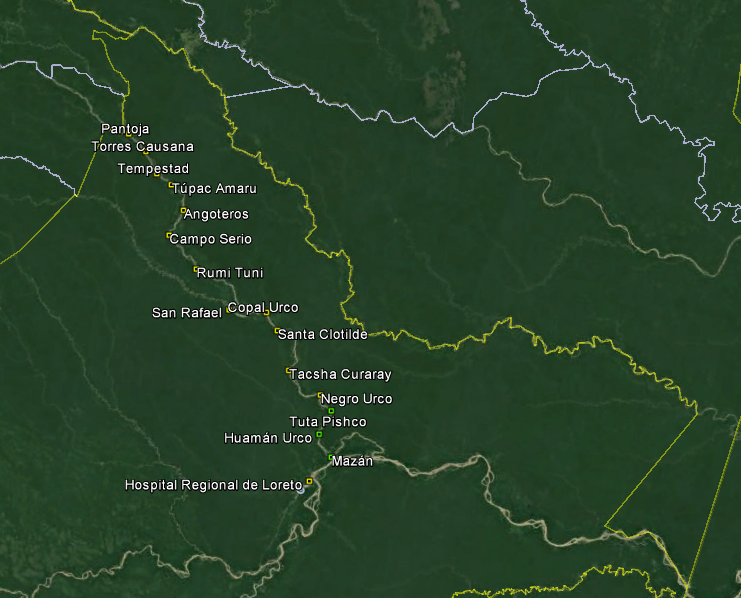
\includegraphics[width=0.7\textwidth]{img/network.png}
		\caption{Localización de la red del Napo}
		\label{NetNapo}
	\end{figure}
	La zona rural comprende desde Cabo Pantoja (cerca de la frontera ecuatoriana) hasta Huaman Urco. Dentro de esta zona, los pueblos más importantes son Cabo Pantoja y Santa Clotilde, debido a que en ellos existen comodidades y servicios básicos para el trabajo.\\
	Por una parte, la zona urbana está formada por el pueblo de Mazán y la ciudad de Iquitos. Por otra parte, el resto de pueblos que forman la red del Napo son pueblos en los cuáles existen limitaciones energéticas y de negocio, por lo que los servicios y prestaciones son precarios.\\\\
	 
	 Posteriormente a su primera etapa como red de telemedicina, operada y mantenida por la Dirección Regional de Salud del Loreto con mucho apoyo de la PUCP, desde 2013 la red fue sometida a una profunda repotenciación y extendida para atender a las necesidades de comunicaciones móviles de la población en general sin dejar de prestar en paralelo los servicios de telemedicina anteriormente citados. La red del Napo está compuesta por la red de transporte (\textit{backhaul}) y la red de acceso. A su vez, la red \textit{backhaul} está formada por enlaces inalámbricos de larga distancia, que utilizan el estándar IEEE 802.11n, desplegados a través de torres ubicadas en los diferentes pueblos que conforman la totalidad de la red. Por otro lado, los servicios de telefonía IP interna, videoconferencia y acesso a Internet,  conforman el total de servicios ofrecidos por la red de telemedicina.\\
	Adicionalmente, la red posee dos accesos satelitales ubicados en Cabo Pantoja y Santa Clotilde, los cuáles ofrecen acceso a Internet a toda la red cuando el tráfico no puede salir a través de la ciudad de Iquitos.
	
	\subsection{Utilización de la red}
	En la nueva red del Napo, deben coexistir dos tipos de red de datos, una de ellas destinada a la telemedicina y otra destinada al acceso 3G. Tanto el acceso a internet de la red de telemedicina, como el de la red 3G será por medio de enlaces satelitales, existiendo dos de ellos para cada una de las redes. Los puntos de acceso satelital para la red de telemedicina estarán ubicados en Cabo Pantoja y Santa Clotilde, mientras que para la red 3G dichas salidas estarán ubicadas en Capo Pantoja y Huaman Urco. En ambas redes se dividirán en grupos las estaciones cliente y se asignarán los accesos satelitales. En caso de indisponibilidad de una pasarela satelital, se reconducirá el tráfico existente por el acceso satelital restante (si éste estuviera disponible).\\\\
	
	Esta nueva red ha de cumplir con todos los requisitos y necesidades individuales de las redes que la componen y, a su vez, debe ofrecer calidad de servicio. Para la coexión de tráficos se ha planteado una implementación de enrutamiento dinámico, separación de tráfico y política de QoS (Calidad de Servicio); todo ello para conseguir acceso a los servicios ofrecidos por cada red y poder acceder, o redirigir, el tráfico a un gateway determinado. A continuación, describiremos los servicios y requisitos mínimos necesarios para cada una de las redes.\\\\
	
	Por un lado, la red de telemedicina compuesta por 16 estaciones clientes (centros y puestos de salud), debe ofrecer servicios internos de telefonía IP, videoconferencia y acceso a Internet. Como se ha mencionado antes, existen dos puntos para el acceso satelital, uno en Cabo Pantoja y otro en Santa Clotilde. Para los servicios de telefonía IP, videoconferencia y acceso a Internet es deseable que todas las estaciones cliente puedan comunicarse de forma simultánea entre sí.\\\\
		
	Por otro lado, la red 3G estará compuesta por 8 centros, los cuáles ofrecerán este servicio. El acceso al Core 3G será por medio de dos enlaces satelitales, ubicados en Huaman Urco y Cabo Pantoja.\\\\
	
	Tras unas primeras pruebas sobre el diseño inicial, recogidas en la tabla \ref{table:RLPUCP} vemos como la capacidad de tráfico más restrictiva por enlace es de 44 Mbps, por tanto se usará este valor como parámetro mínimo en cuanto a capacidad para el resto de radioenlaces. Otra restricción a tener en cuenta es la climatológica, puesto que la red es extensa y existe la posibilidad de que diferentes situaciones degraden la señal.
		
\section{Objetivos del proyecto}
	El objetivo del proyecto Napo es implementar el servicio de acceso de telefonía móvil, provisto de celdas 3G, para que sea compatible con los servicios ya existentes en la red de telemedicina. Para ello, se reemplazarán los equipos de los emplazamientos involucrados en el proyecto. La finalidad de este cambio es mejorar las capacidades de los enlaces radio, para la coexión de tráfico de telefonía celular 3G y los servicios de telemedicina. En orden con lo anterior, para el acceso al Core 3G, se desarrollarán dos nuevos accesos satelitales ubicados en Cabo Pantoja y Huaman Urco.\\\\
	
	El objetivo de este Trabajo Fin de Grado consiste en proporcionar una solución sostenible al proyecto, capaz de adaptarse a las situaciones y limitaciones del mismo, y que mantenga los mínimos criterio respecto a los diferentes niveles de QoS definidos en el proyecto. Este trabajo se hace en cooperación internacional con el equipo de ingeniería del GTR (Grupo de Telecomunicaciones Rurales) de la PUCP, que son responsables en el proyecto Napo de tomar muchas de las decisiones de diseño. De esta forma, en este trabajo se realizará fundamentalmente una cooperación para la toma de decisiones de diseño, y una auditoría técnica para verificar que dichas decisiones cumplen con las especificaciones previas de la red. Para ello, se realizarán configuraciones equivalentes a las existentes en la nueva red del Napo en laboratorio y se propondrán soluciones respecto a la gestión y monitorización de la red, todo ello mediante el uso de un software dedicado.
	 
\section{Organización del documento}
	La organización correspondiente al Trabajo Fin de Grado viene detallada a continuación.\\\\
	
	En el primer capítulo, se hace una introducción al desarrollo de las TIC en América latina y, más en concreto, al contexto existente en la cuenca del río Napo. Se presenta la red desplegada en el proyecto TUCAN3G mostrando los resultados obtenidos, y procediendo a su posterior análisis. Por último, se detalla la relación del proyecto Napo con el Trabajo Fin de Grado.\\\\
	
	En el segundo capítulo, se describirá el estado del arte referente a las diferentes tecnologías y protocolos utilizados en el proyecto. Por un lado, se realizará una descripción de las soluciones propuestas para redes de transporte en zonas rurales. Por otro lado, se introducirá la monitorización y gestión de redes para nuestro trabajo, y se describirán las diferentes soluciones software posibles.\\\\
	
	En el tercer capítulo, se explicará de manera detalla, el funcionamiento y configuración de los equipos involucrados en el Trabajo Fin de Grado, teniendo como objetivo obtener un escenario similar al que pudiera tenerse en el marco del proyecto. Para ello, se realizarán pruebas a nivel de laboratorio referentes a tráfico y monitorización de los equipos.\\\\
	
	En el cuarto capítulo, se procede a analizar y contrastar los resultado obtenidos. Dichos resultados deberán aportar una solución en cuanto a los requisitos de diseño de la nueva red del Napo y detectar anomalías si las hubiera.\\\\
	
	En el quinto capítulo, se muestran las conclusiones  y competencias adquiridas a partir de este Trabajo fin de Grado, y una visión acerca de futuros trabajos basados en este proyecto.\\\\
	
	En el sexto capítulo, se muestran las tablas y código utilizado para el desarrollo de este Trabajo Fin de Grado.\\\\
	
	Finalmente, se encuentra la bibliografía utilizada para llevar a cabo este Trabajo Fin de Grado.
	\chapter{Marco teórico}
\label{cap:marco_teorico}
	En este capítulo se explicarán de manera resumida los conceptos y tecnologías más importantes relacionadas con el desarrollo del proyecto, así como una breve introducción a la monitorización de redes.\\
	
	A continuación, se describirán las soluciones y propuestas empleadas para resolver el problema sobre la red de transporte. Así mismo, se explicarán los estándares y protocolos utilizados. En concreto, se hablará de las tecnologías inalámbricas: WiFi, haciendo un aparte sobre su modalidad relacionada con largas distancia (WiLD), WiMAX, LTE, \textit{Television White Spaces} (TVWS) y los protocolos propietarios de Mikrotik \cite{Mikrotik} Nstreme y NV2.\\
	
	Por un lado, se detallará la legislación y normativa vigente en el marco del proyecto respecto al uso y despliegue de dichas tecnologías, acorde con el artículo \cite{espinoza2018wireless}. Y por otro lado, se hará una introducción a la calidad de servicio y tráfico en redes, detallando lo más importante de cada una de las arquitecturas involucradas el desarrollo de este Trabajo Fin de Grado.\\
	
	Por último, se analizarán diferentes programas \textit{software} de gestión de redes cuya funcionalidad encaja con las necesidades de este proyecto, y se establecerá una comparativa entre ellos. Del mismo modo, se comentará de manera más detallada el funcionamiento y características de la herramienta escogida como solución para el desarrollo del proyecto.
	
\section{Red de transporte en redes inalámbricas para zonas rurales}
	Como ya se ha comentado, la extensión de la cobertura de redes de telecomunicaciones en zonas rurales tropieza con el hándicap del elevado coste de despliegue de las infraestructuras necesarias frente a una expectativa de bajo retorno de la inversión, debido a la escasa densidad de población de estas zonas; este problema es mayor cuanto menor es la densidad de población, mayor la distancia focos de concentración, y menor el poder adquisitivo de la población. Por tanto, existe la necesidad de soluciones flexibles y de bajo coste para tratar de resolver dicho problema.\\
	
	En lo que respecta al acceso radio en redes de comunicaciones móviles de banda ancha, una solución que se ha aplicado en algunos proyectos, como es el caso del TUCAN3G, es el uso de femtoceldas. Las femtoceldas son estaciones base diseñadas para servir a un reducido número de usuarios concurrentes y con una potencia de transmisión también muy pequeña, y se asume que usan como \textit{backhaul} un enlace de acceso a Internet pre-existente; en un principio estaban diseñadas para cubrir los huecos de cobertura existentes en determinadas zonas, por lo cual muchas de ellas están alojadas dentro de edificios. Lo que hace de las femtoceldas una solución viable es su bajo coste, su escaso consumo energético y su flexibilidad y sencillez de despliegue. Esto aporta una solución más viable para el operador de telefonía frente al uso de nodos convencionales: la inversión es menor, obteniéndose un redimiento adecuado.\\
	
	Por otra parte, para transportar el tráfico intercambiado entre estas redes de acceso y la red fija de transporte del operador, hace falta también una solución igualmente apropiada para el transporte rural. Se requieren tecnologías de muy bajo costo y flexibles para que al operador le traiga cuenta desplegar tal infraestructura, o incluso compartirla con otros agentes socioeconómicos. A continuación se procede a explicar brevemente el funcionamiento de las distintas tecnologías pertenecientes al ámbito de comunicaciones inalámbricas para enlaces de larga distancia, obteniendo así diferentes rendimientos de la solución propuesta.


\section{Protocolos Inalámbricos}

		\subsection{Nstreme}
		El protocolo Nstreme es un protocolo inalámbrico, que posteriormente daría lugar al protocolo NV2, y que utiliza \textit{polling} como técnica de acceso al medio correspondiente a la capa \cite{MacLayer}. El funcionamiento del protocolo viene ilustrado en la Figura \ref{Nstreme}. Siguiendo con este protocolo, la comunicación entre estaciones base se produce de manera independiente a la comunicación con los nodos cliente. La comunicación entre clientes y estaciones base se realiza utilizando mensajes de señalización, o \textit{tokens}, con los que las estaciones base conocen el comienzo y final de la transmisión. Si la estación base considera que un nodo cliente no está emitiendo pasaría a inspeccionar otro nodo de la red.    
	
		\begin{figure}[H]
			\centering
			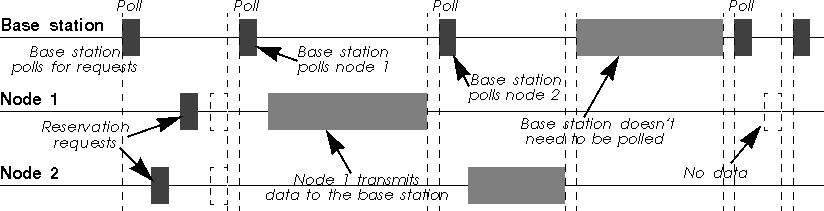
\includegraphics[width=0.7\textwidth]{img/Polling.png}
			\caption{Funcionamiento \textit{Polling} en Nstreme. Fuente: IJCAT}
			\label{Nstreme}
		\end{figure}
		
		Acorde con esto, las ventajas e incovenientes del protocolo son:
		\begin{itemize}
			\item No existen limitaciones entre estación base y cliente.
			\item Baja sobrecarga de cabeceras en las tramas, por lo que permite conseguir mayores tasas de envío.
			\item Retardo por propagación y latencia como consecuencia de usar \textit{polling}.
		\end{itemize}

		\subsection{NV2}
		El protocolo NV2 es un protocolo inalámbrico, perteneciente a la capa MAC \cite{MacLayer}, basado en el acceso múltiple por división de tiempo (TDMA) en lugar de \textit{polling} o acceso múltiple con escucha de señal portadora (CSMA). Este último es el usado más comúnmente por la mayoría de equipos relacionados con el estándar IEEE 802.11.\\
		
		Para explicar el funcionamiento del protocolo NV2, ilustrado en la Figura \ref{NV2}, vamos a suponer un escenario en el cual nuestra red estará compuesta por una estación base (BS) y diferentes clientes que comparten BS mediante este protocolo. El acceso al medio de los clientes estará organizado por la BS, que dividirá el tiempo en períodos. Estos períodos estarán dinamicamente divididos en porciones para \textit{Downlink} (datos enviados desde la BS hacía el cliente) y \textit{Uplink} (datos enviados desde el cliente a la BS). Al comienzo de cada período, la BS mandará un mensaje mediante \textit{broadcast} a los clientes con información sobre en qué momento han de transmitir y del tiempo disponible para ello. \\
		Acorde con lo anterior, la BS de manera periódica asigna una parte del tiempo de Uplink para un "cliente desconocido". Dicho tiempo tiene como objetivo favorecer la integración y comunicación de un nuevo cliente con la red (si lo hubiera). Para ello, la BS estima el retardo que existe entre la comunicación existente y el nuevo cliente reajustando el tiempo de Uplink, permitiendo completar el registro y comunicación del nuevo cliente con la red.
		
		\begin{figure}[H]
			\centering
			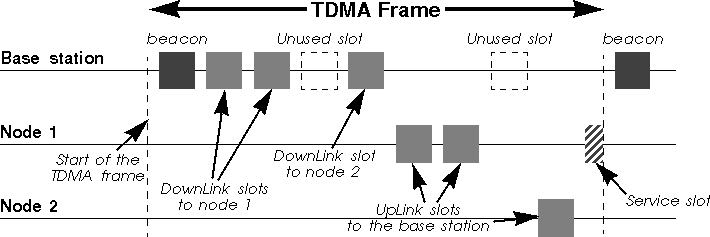
\includegraphics[width=0.7\textwidth]{img/TDMA.png}
			\caption{Funcionamiento TDMA en NV2. Fuente: IJCAT}
			\label{NV2}
		\end{figure}
		
		Las ventajas e inconvenientes del protocolo NV2 se detallan a continuación:
		\begin{itemize}
			\item Mejor rendimiento en redes punto a punto (PTP).
			\item Mayor \textit{throughput} y menor latencia.
			\item No existe el problema del nodo oculto.
			\item Únicamente se podrán establecer redes homogéneas al protocolo NV2, en consecuencia podrá existir interferencia entre redes que no usen NV2 y viceversa.
		\end{itemize}
		
\section{Tecnologías Inalámbricas}
Antes de comenzar con el análisis sobre las diferentes tecnologías inalámbricas estudiadas en el marco del proyecto,  debemos de tener en cuenta todas la limitaciones existentes en el proyecto Napo. Esto implica no sólo el coste e inversión económica que ha de hacerse para desarrollar una infraestructura de telecomuniaciones viable, sino que también debemos tener en cuenta las normas y legislaciones existentes en cuanto al uso del espectro radioeléctrico peruano.\\

Durante las últimas décadas, las telecomunicaciones en áreas rurales de América Latina han sufrido fuertes barreras y obstáculos frente a la implantación de un modelo de desarrollo sostenible. La poca densidad y dispersión de poblaciones con bajo poder adquisitivo no suponen un aliciente para los operadores de telecomunicación, e incluso a veces tampoco para las administraciones públicas. En la medida en que las TIC son soporte para toda la actividad humana, eso ha influido en que de manera general el acceso a servicios básicos en zonas rurales se haya distanciado aún más del existente en las urbes.\\

Como cosecuencia de esto, en 2005 el ministerio peruano de transporte y comunicaciones (CTM), aprobó una nueva ley sobre el uso del espectro radioeléctrico a nivel nacional. Con el objetivo de utilizar dicho espectro de forma más eficiente y promover el despliegue de nuevas redes inalámbricas, se redefinieron los usos y asignaciones de las bandas disponibles en el espectro, tratando de satisfacer así la fuerte demanda creciente en cuanto a servicios TIC. Esta clase de políticas han ido en paralelo a la fuerte apuesta por extender las infraestructuras de comunicaciones ópticas que interconectan los focos de concentración de la población (ciudades y pueblos grandes); las comunicaciones inalámbricas, más allá de las comunicaciones móviles, se han visto como la manera de llegar allá donde las infraestructuras de fibra no son costo-eficientes, pues en esos contextos las tecnologías inalámbricas tienen una mayor flexibilidad, requieren una inversión inicial de capital menor meintras que su despliegue y desarrollo son más rápidos.\\

A continuación, analizaremos el espectro readioeléctrico en el contexto peruano, así como el uso, aplicación y evolución de las diferentes tecnologías que han sido objeto de estudio durante la realización de este Trabajo Fin de Grado.

\subsection{WiFi}
La tecnología WiFi surge originariamente como solución a las necesidades de redes inalámbricas locales (WLAN). No obstante, desde su primera versión del estándar IEEE 802.11 con perfiles como 802.11a y 802.11b, y hasta las últimas 802.11ac, esta tecnología ha sido adaptada para su utilización como solución a los problemas de comunicaciones inalámbricas para redes metropolitanas y redes rurales de forma creciente. La principal característica de WiFi es su mecanismo de acceso al medio basado en CSMA/CA (\textit{Carrier Sense Multiple Access/Collision Avoidance}) perteneciente a la familia de CSMA, que determina la forma de repartir el canal compartido para una estación que desea transmitir. El funcionamiento de CSMA se basa en la búsqueda de una portadora reconocida en el medio compartido para otorgar el turno de transmisión a la estación que desea transmitir sólo si no hay tal detección de portadora, evitando así colisiones entre estaciones que tienen en curso una transmisión y estaciones que desean empezar a transmitir. La variante CSMA/CA está optimizada para canales radio, minimizando así el problema de las colisiones con diversas técnicas que se complementan entre sí.\\

Gracias al avance del estándar, las tasas registradas para esta tecnología pueden alcanzar los 600 Mbps teóricos (tasa binaria) y entorno a los 300 Mbps de caudal en las estaciones que incorporan las enmiendas más recientes del estándar (a partir de 802.11n); estas estaciones se denominan formalmente HT-STAs (\textit{High Throughput STAtions}), a diferencia de las non-HT-STA cuyos mecanismos de las capas PHY y MAC no permitirían alcanzar tasas tan altas al no incorporar los últimos avances del estándar.\\

Por un lado, en la capa MAC los cambios respecto a las estaciones non-HT-STA son referentes a la agregación de tramas, uso de protocolo de dirección inversa, reducción de tiempos de espera y mecanismos de coexistencia con non-HT-STA. Por otro lado, en la capa PHY la principal mejora es la introducción y soporte de MIMO que permite la multiplexación espacial. \\

Aunque con posterioridad a 802.11n ha tenido también un fuerte impacto el uso de la nueva enmienda 802.11ac, en el caso de las comunicaciones WiFi aplicadas a largas distancias el gran salto se produjo con 802.11n gracias a la introducción del MIMO y de la agregación de tramas y otros mecanismos complementarios para aumentar la eficiencia de las transmisiones. A continuación se detallan nuevas mejoras y técnicas aplicadas al estándar 802.11n, con el objetivo de mejorar las prestaciones y eficiencia del mismo acorde con las estaciones HT:
\begin{itemize}
    \item Ampliación del espectro de 20 MHz a 40 MHz, agrupando canales consecutivos de 20 MHz y considerando de 1 MHz el tamaño de las bandas de guarda, lo que permite duplicar la información contenida dentro del canal.
    
    \item Dualidad de canales a la hora de seleccionar una frecuencia de trabajo u otra , es decir, utilizar las frecuencias de 2,4 y 5 GHz indistintamente, permitiendo así que exista retrocompatibilidad con todas las versiones de WiFi.
    \item Mejora de agregación de tramas sobre capa MAC basada en la agrupación global de tramas mediante las técnicas de A-MDSU (\textit{Aggregate MAC Service Data Unit}) y A-MPDU (\textit{Aggregate MAC Protocol Data Unit}). \\
    
    Por un lado, la técnica A-MDSU se aplica al inicio de la capa MAC y consiste en agregar múltiples MSDU (\textit{MAC Service Data Unit}) como primer paso al formar la trama totalitaria MPDU (\textit{MAC Service Data Unit}). Por otro lado, la técnica A-MPDU se efectúa al final de capa MAC agregando múltiples MPDU (\textit{MAC Protocol Data Unit}) transportadas como una simple PSDU (\textit{Protocol Service Data Unit}) por la capa PHY.\\
    
    En conclusión, el uso de estas técnicas permite reducir la transmisión de cabeceras debido a que la trama de datos será enviada en una única transmisión, utilizando el medio compartido de forma más eficiente.
    
    \item Transmisiones múltiples sin necesidad de esperar un tiempo excesivo reduciendo el acceso total al medio y aumentando la eficiencia de la red. Para esto se utilizan los mecanismos de RIFS (\textit{Reduced InterFrame Space}) y SIFS (\textit{Short InterFrame Space}).
    
    \item Modulación y codificación determinada por los equipos para establecer comunicación entre ellos. Definimos MCS (\textit{Modulation and Coding Schema}) como el esquema existente en los equipos para comunicarse a través de una modulación determinada. Actualmente, existen 127 MCS para el estándar 802.11n, no obstante en este Trabajo Fin de Grado sólo han sido utilizadas las MCS comprendidas entre MCS8 y MCS15 destinadas a diversidad espacial en transmisión 2x2 (MIMO 2x2).
\end{itemize}

\subsubsection{WiLD: WiFi para Largas Distancias}
Como hemos comentado en el apartado anterior, WiFi utiliza el protocolo CSMA/CA para acceder al medio, lo que implica que no sea del todo satisfactorio en el ámbito de comunicaciones inalámbricas de largo alcance, ya que los tiempos de silencio en el canal necesarios para esta clase de control de acceso al medio se hacen insuficientes para evitar las colisiones o, si se agrandan fuera de lo que marca el estándar, tienen un alto impacto en la eficiencia. No obstante, esto no hace que el uso de WiFi se deseche por completo ya que, realizando un pequeño ajusta al funcionamiento del protocolo de acceso al medio y asegurando una linea de visión directa entre los enlaces conseguiremos una solución viable en nuestro contexto.\\
		
WiFi es usado principalmente en canales cuyo ancho de banda se corresponde a 20 MHz. Sin embargo, su uso para canales de 5 y 10 MHz es también posible desde las primeras versiones del estándar, y a partir de la revisión IEEE 802.11n es también posible emplear canales de 40 MHz, e incluso de 80 MHz a partir de la 802.11ac. Adicionalmente, desde IEEE 802.11n la transmisión y recepción de señal existiendo diversidad espacial es posible, ya que la mayoría de equipos están diseñados con antenas duales MIMO 2x2. Otra característica que ofrece WiFi es su funcionamiento respecto a la agregación de tramas, ya que podemos crear una trama de mayor tamaño manteniendo una única cabecera y siendo capaces de establecer una diferenciación en el tráfico. \\
		
Aunque el estándar ofrece mejoras en la capa física, tendremos que tener en cuenta otros parámetros como la potencia de señal recibida (SNR), la modulación y códigos utilizados para obtener una tasa de transmisión óptima en nuestra red. Teniendo en cuenta todo esto, WiFi podría ser una solución viable y sostenible en el marco de nuestro proyecto. Sin embargo, debemos tener en cuenta el rendimiento que ofrece el estándar frente al canal utilizado y su gestión de acceso al medio. Del mismo modo, hay que tener en cuenta la gran distancia existente entre las estaciones y la diversidad climotológica existente a lo largo de la red.\\

Acorde con el artículo \cite{simo2014assessing}, vemos como el rendimiento de WiFi en largas distancias no es del todo óptimo, debido a su uso de CSMA/CA como protocolo de acceso al medio. Por ello, a menudo los productos \textit{WiFi Outdoor} de las diferentes marcas implementan alguna clase de alternativa  a CSMA/CA basada en TDMA (\textit{Time Division Multiple Access}) que mejora considerablemente el rendmiento del \textit{hardware} WiFi a distancias largas al evitarse constantes colisiones que tienen un impacto muy negativo en la eficiencia de los enlaces en esas condiciones. Independientemente del protocolo utilizado en la capa MAC, cualquier \textit{hardware} que utilice el estándar 802.11 y que esté basado en los \textit{chipsets} más flexibles de últimas generaciones tendrá las características mencionadas anteriormente. \\

\subsubsection{Marco legislativo}
En 2008 el CTM determinó para Perú las bandas destinadas a la tecnología WiFi en las siguientes frecuencias: 902-928 MHz, 2,4-2,483.5 GHz, 5,725-5,850 GHz, 5,250-5,350 GHz y 5,470-5,725 GHz. Dichas bandas estaban destinadas a los servicios de telecomunicaciones en zonas rurales y áreas en las cuales no se requería el uso de banda licenciada. \\

Posteriormente, durante el 2011 y hasta el 2013 está legislación sufrió algunas actualizaciones, conviertiendo la banda de 902-915 MHz en una banda licenciada para el uso de servicios de telecomunicaciones. Por tanto, el CTM tuvo que reestructurar está repartición del espectro. Dicho rediseño se llevó a cabo en 2013 y, como resultado, las bandas de frecuencias utilizables por WiFi en Perú quedaron de la siguiente manera: 916-928 MHz, 2,400-2,483.5 GHz, 5,725-5,850 GHz, 5,250-5,350 GHz y 5,470-5,725 GHz.\\

El CTM redistribuyó el espectro radioeléctrico a consecuencia de la fuerte demanda de servicios de telecomunicaciones existente. Dicha reforma garantizaba la viabilidad de los servicios en redes ya existentes, y promovía el despliegue de nuevas redes que aportarán una solución frente a la fuerte demanda. \\

		
\subsection{WiMAX}
El estándar IEEE 802.16, más comunmente conocido como WiMAX, fue diseñado para su uso en áreas metropolitanas, aunque sus características hacen de esta tecnología una candidata natural para el despliegue de redes inalámbricas rurales de banda ancha a punto fijo. Si bien el estándar IEEE 802.16 especifica el uso de esta tecnología en distintas bandas de frecuencias, y uno de los perfiles es para bandas no licenciadas en 5 GHz, el consorcio de empresas conocido como WiMAX Forum, responsable de certificar la compatibilidad e interoperabilidad de productos en el marco de este estándar, no ha reconocido un perfil para bandas no licenciadas. Por lo tanto, existen equipos IEEE 802.16 que funcionan en banda libre de 5 GHz, pero formalmente no podrían usar la denominación WiMAX. El protocolo de acceso al medio de este estándar es TDMA y la técnica de transmisión utilizada es OFDM.\\

La capacidad óptima en un radioenlace que utiliza WiMAX depende, entre otros factores, de la modulación que se consiga transmitir, la codificación utilizada, el tamaño de la trama que deseemos enviar y el intervalo de guarda existente entre los símbolos OFDM. Acorde con el artículo \cite{simo2014assessing} las tasas obtenidas si utilizamos WiMAX en enlaces de larga distancia, pueden estar comprendidas entre 1.6 Mbps y 33 Mbps, eso en el mejor de los casos con tramas de 20 ms de duración.\\
		
Aunque los sistemas de comunicaciones que utilizan los estándares 802.11 y 802.16 en bandas no licenciadas tienen un bajo coste, tanto por el precio de los equipos como por la posibilidad de utilizar el espectro sin pagar licencias, su despliegue si entraña costes nada desdeñables por el diseño y construcción de estructuras de soporte para ubicar los sistemas de comunicación y las antenas a las elevaciones necesarias para enlaces de largas distancias, con el objetivo de mantener línea de visión directa. Dependiendo del contexto geográfico y de la distancia comprendida entre focos de concentración de población, la instalación de estas estructuras de soporte pueden ser un coste muy dominante que hagan muy costoso el despliegue de las infraestructuras de transporte con independencia del equipamiento de comunicaciones usado. Aparte de esto, la transmisión de potencia en bandas no licenciadas se debe tener en cuenta, pues existen restricciones de límites de potencia (independientemente de la tecnología que se emplee), lo que condicionan la viabilidad de nuestros enlaces.

\subsubsection{Marco legislativo}
En el año 2005 y con el objetivo de mejorar el acceso a los servicios de telecomunicaciones mínimos, el CTM destinó las bandas de 3,4-3,5 GHz y 3,5-3,7 GHz (también conocidas como bandas 3,4) para dicho objetivo. Aparte de este reparto, el CTM dictaminó que los operadores que quisieran obtener un canal en las bandas ya mencionadas deberían limitarlo a un tamaño máximo de 50 MHz, independientemente del área geográfica en cuestión.\\\\

En el 2006, este espectro volvió a sufrir otra redistribución, dejando las bandas comprendidas entre las frecuencias de 2,5-2,692 GHz para el acceso público a servicios mínimos de telecomunicaciones. Dicho rediseño trajo consigo una subasta de parte del espectro por parte del MTC, garantizando el uso de bandas libres de impuestos en Lima. A lo largo de 2007, el MTC se dio cuenta que dichas bandas tenían un gran potencial en cuanto a rentabiliadad y rendimiento, por lo tanto decidieron dedicar esas bandas a mejorar el uso de servicios móviles mediante el uso de WiMAX.\\\\

Este último hecho no suponía una tarea sencilla, ya que parte del espectro tenía que volver a ser restructurado y esto implicaba una inversión económinca adicional para recuperar la licencia de las bandas antes mencionadas. Con el objetivo de ampliar la infraestructura de redes y mejorar el acceso a las ya existentes, en 2010 se llevó a cabo otra reestructuración del espectro. Esto implicó una inversión de capital adicional ya que muchas bandas habían sido licenciadas.

\subsection{LTE}
La tecnología LTE (\textit{Long Term Evolution}) es un estándar para comunicaciones inalámbricas de transmisión de datos a alta velocidad para terminales de datos y dispositivos móviles. Esta tecnología pertenece al grupo de tecnologías englobadas dentro del 3GPP (\textit{The 3rd Generation Partnership Project}\cite{3gpp}) cuyo principal objetivo es ofrecer acceso inalámbrico a servicios móviles, dentro de esta familia destacan los estándares GSM (\textit{Global System for Mobile communications}) de segunda generación y UMTS (\textit{Universal Mobile Telecommunications System}) clasificado de tercera generación. El estándar UMTS fue diseñado como evolución de GSM y aparte de obtener una mayor tasa de transmisión, su principal diferencia es el protocolo de acceso al medio ya que UMTS utiliza W-CDMA (\textit{Wideband Code Division Multiple Access)} como protocolo de acceso al medio.\\

Como siguiente paso en el proceso evolutivo de dichas tecnologías aparece LTE, cuyas prestaciones mejoran respecto a los anteriores estándares, entre otras cosas debido al uso de OFDMA en el enlace descendente y SC-FDMA en el ascendente. Este cambio implica aumentar la tasa de transmisión instántanea a valores de 100 Mbps en el \textit{downstream} y 30 Mbps en el \textit{upstream}.\\

El siguiente paso en lo que a este estándar se refiere es el denominado LTE-A (\textit{LTE Advanced}) que ofrece tasas de transmisón mucho mayores en enlaces radio y una mejora en la arquitectura de LTE.

\subsubsection{Marco legislativo}
Desde 2005, el MTC permitía a los operadores de telecomuniaciones adquirir bandas licenciadas con un máximo de 60 MHz para ofrecer sus servicios. Dicho modelo estaba enfocado a mantener la viabilidad y competitividad en el mercado de las telecomunicaciones en cuanto al acceso público a redes. El espectro que se ofertaba y el que era accesible por parte de las operadoras era el comprendido entre 700, 800, 900 y 1900 MHz. En 2010, este espectro fue identificado como una barrera para el desarrollo e implementación de acceso a nuevas redes, tanto en un entorno urbano como en un entorno rural. Como resultado de esto, se estableció un nuevo plan de políticas y regulaciones con el objetivo de maximizar el rendimiento del espectro actual teniendo en cuenta la aparición de nuevas tecnologías y las exigencias del mercado de las telecomunicaciones.\\

En el 2011, por un lado las operadoras ofrecían sus servicios de acceso a la red en las bandas de 800 y 1900 MHz, y por el otro, el MTC alojaba bandas adicionales para promover el acceso a nuevos servicios públicos de telecomunicaciones. Dichas bandas son las siguientes: 894 - 902 MHz, 939-947 MHz, 902-915 MHz, 947-960 MHz 1,710 - 1,770 GHz, 2,110 - 2,170 MHz, 902-915 MHz y 947-960 MHz. Todas estas bandas fueron subastadas a las operadoras, lo que manifestaba una creciente demanda en cuanto al desarrollo de nuevas redes de acceso utilizando nuevas tecnologías.\\

En 2013, el MTC realizó una modificación en la regulación de uso del espectro. Esta nueva regulación estaba enfocada a modificar los 60 MHz que imponían a las operadoras, ya que en muchos casos se estaba alcanzando e incluso sobrepasando dicha capacidad. Para ello, se mantuvo el uso de 60 MHz en las bandas de 800, 900 y 1900 MHz mientras que en las bandas de 1,7 y 2,1 GHz se ofertaban 80 MHz en total, divididos en dos franjas de 40 MHz ubicadas cada una de ellas en diferentes partes del espectro. El uso creciente de tecnologías 4G-LTE provocó que el MTC subastará dos bloques dedicados en las bandas de 1,7 y 2,1 GHz para dicha tecnología.

\section{Gestión del tráfico y QoS en redes}

\subsection{QoS: Calidad de Servicio}
La calidad de servicio (QoS, \textit{Quality of Service}) se define como la capacidad de una red de telecomunicaciones de satisfacer un determinado tipo de servicio o una serie de servicios, en función de los niveles alcanzados en ciertos parámetros observables a nivel de usuario y de aplicaciones. Los servicios que debemos tener en cuenta a la hora de medir la QoS soportada de la nuestra red son la utilización de ancho de banda, las presaciones alcanzadas en el envío y recepción de paquetes y la capacidad de gestión del tráfico (clasificación, priorización, conformado, control de la congestión, etc.) para garantizar para cada tipo de tráfico el tratamiento que necesita para el correcto funcionamiento del correspondiente servicio.\\

Todas las aplicaciones que sean destinadas a dar un servicio a usuarios finales deben garantizar un mínimo de QoS. Para cumplir esto, no sólo es importante el conjunto de la red sino que además cada elemento de forma individual debe estar alineado con la red para mantener el nivel de QoS total. Las redes de telecomunicaciones en mayor o menor medida son redes no homogéneas, es decir, tenemos elementos que actúan en capas diferentes, pueden ser de fabricantes diferentes, tienen mecanismos de interacción con la red diferentes, tiene arquitectura diferentes, etc. En consecuencia de esto, es importante establecer umbrales en ciertos parámetros medibles para cada tráfico que permitan proporcionar un buen nivel de QoS a las diferentes aplicaciones. Estos parámetros suelen ser los siguientes:

\begin{itemize}
    \item \textit{Throughput} (bps): Tasa a la que se pueden transmitir datos.
    \item Retardo (ms): Diferencia de tiempo transcurrido entre el envío y recepción de paquetes.
    \item \textit{Jitter} (ms): Variación del retardo.
    \item Paquetes pérdidos (\%): Porcentaje de paquetes pérdidos durante el envío.
\end{itemize}

A la hora de valorar el rendimiento que está ofreciendo la red a los usuarios y aplicaciones finales, no sólo hay que tomar en cuenta los factores comentados anteriormente sino también el tipo y la intensidad de tráfico existentes en la red. El tráfico existente en una red se produce por flujos asociados a agregaciones de paquetes de las mismas características y servicios iguales o asimilables que recorren la red desde un emisor hacia un receptor en el mismo sentido y requieren el mismo tratamiento. Los paquetes de distintos flujos pueden ser clasificados y jerarquizados con arreglo a determinada política de prioridades y de tratamiento de las distintas clases de tráfico observando las cabeceras de los paquetes, y concretamente campos tales como direcciones IP destino y origen, puerto, etc.\\

Generalmente en las fronteras de cada red y subred se suele hacer una diferenciación del tráfico según el tipo para poder establecer prioridades entre las distintas clases de tráfico existentes y tratar de garantizar a cada una, o al menos en la medida de lo posible, la QoS que se necesita para un correcto funcionamiento de los servicios. Este proceso de clasificación de tráfico puede asociar a cada clase diferenciada varios flujos, es decir, puede diferenciarse un conjunto relativamente bajo de clases de tráfico agregando flujos que requieren idéntico tratamiento dentro de una misma clase, para obtener un soporte adecuado de QoS al tiempo que se hace escalable a medida que la red y su carga de tráfico crecen. 

\subsection{Gestión del tráfico en redes}
Para sostener un determinado nivel de servicio y una determinada QoS para los diferentes servicios, es preciso un correcto diseño y planificación de la red, y una adecuada distribución de los recursos de la red. No obstante, esto no es suficiente porque a partir del momento en que la red se pone en funcionamiento, no cesan de producirse cambios, unos transitorios y otros permanentes, en el estado de los sistemas de la red, en la demanda de uso que hacen los usuarios, en el estado de los canales, etc. Lo que inicialmente funciona según las previsiones, pronto deja de hacerlo y, en consecuencia, no se puede asegurar que la red cumpla con sus objetivos sin observar de forma muy precisa y constante cómo la red y su entorno cambian y sin actual ante esos cambios en consecuencia.\\

El campo técnico relativo a la observación o monitorización eficaz y eficiente de la red, y a la actuación efectiva sobre ésta ante los cambios de las necesidades o del estado de la red, se denomina \textit{gestión de redes}.\\

A continuación se comentan algunas cuestiones teóricas relacionadas con la gestión de redes.
	
	\subsubsection{Disciplinas de colas}
Las disciplinas de colas son las diferentes estrategias para gestionar el tráfico que transita por un dispositivo de red, principalmente un router, para elegir el siguiente paquete que será enviado por la red, y para manejar los parámetros de calidad que se pretenden lograr. Tal y como se muestra en la Figura \ref{teoriaColas}, los paquetes que llegan al dipositivo por la interfaz de entrada son encolados en un \textit{buffer} de salida y el paquete seleccionado se enviará por la interfaz de salida; dicha elección está determinada por el algoritmo de colas que utilice el dipositivo.
	
	\begin{figure}[H]
			\centering
			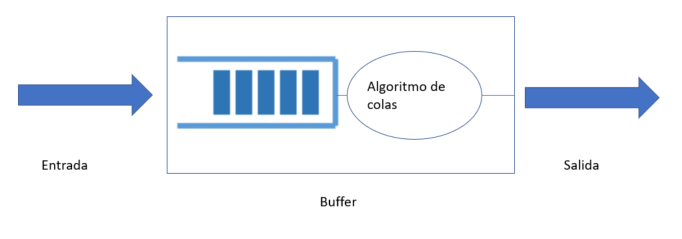
\includegraphics[width=0.7\textwidth]{img/teoriaColas.PNG}
			\caption{Esquema del funcionamiento de encolado en un \textit{router}.}
			\label{teoriaColas}
		\end{figure}
		
	La disciplinas de colas apropiadas dependen del tipo de tráfico existente en la red. Hay dos grandes grupos de disciplinas de colas: sin clases y con clases. La principal diferencia es la diferenciación que se realiza por clases, procesando de forma diferente el tráfico según el tipo de clase al que esté asociado. Solo a modo de ejemplo, sin ser en absoluto una relación exhaustiva de las alternativas, se procede a comentar brevemente algunas de las disciplinas de colas o \textit{qdiscs} más sencillas:
	
	\begin{itemize}
	    \item FIFO (\textit{First In First Out}): Este método consiste en enviar los paquetes en el orden de llegada que fueron recibidos, tal y como muestra la Figura \ref{fifolifo}. Es el más utilizado, ya que es el que gran parte de los dispositivos usan por defecto.
	    \item LIFO (\textit{Last In First Out}): Al contrario que FIFO este método consiste en reordenar y enviar los paquetes en el orden inverso al que fueron llegando, ilustrado en la Figura \ref{fifolifo}. Siendo el último paquete recibido el primer en ser enviado. 
	    \item PRIO: Este método tiene como base el mecanismo FIFO, no obstante lo destacable de este método es la previa jerarquización a la que son sometidos los paquetes. Primeramente, los paquetes pasan por un filtrado y acto seguido son ubicados en la cola correspondiente según su clasificación, enviando de manera más rápida los paquetes cuya prioridad es más alta. 
	\end{itemize}
	
	\begin{figure}[H]
			\centering
			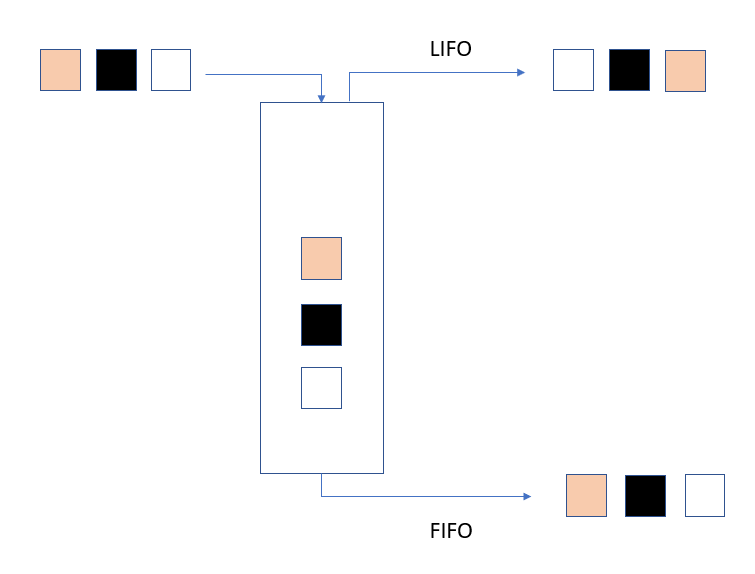
\includegraphics[width=0.7\textwidth]{img/fifolifo.PNG}
			\caption{Esquema del funcionamiento de las teorías FIFO y LIFO.}
			\label{fifolifo}
		\end{figure}

	\subsubsection{DiffServ} 
	La arquitectura DiffServ (Servicios Diferenciados) es una arquitectura de red que permite clasificar el tráfico diferenciando según los diferentes niveles de QoS, es decir, pueden coexistir varios flujos en la red, los cuales serán tratados y diferenciados en función de la QoS que necesitan. Esto se realiza con el fin de diferenciar cada tipo de tráfico del resto, e impedir por ejemplo que clases de tráfico más exigentes en lo relativo a la QoS se vean afectadas negativamente por la presencia de un tráfico intenso de otras clases que, posiblemente, no necesiten del mismo tratamiento y puedan ver rebajada su prioridad sin gran impacto sobre los servicios a los que corresponden. Para entender esta arquitectura es importante introducir los términos de \textit{router} frontera (color azul) y \textit{router} núcleo de red (color naranja); la Figura \ref{diffserv} muestra un escenario base que utilizaremos para explicar dichos términos y explicar su función dentro de esta arquitectura.
	
	\begin{figure}[H]
			\centering
			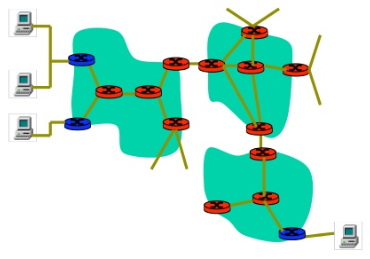
\includegraphics[width=0.5\textwidth]{img/diffserv.PNG}
			\caption{Ejemplo de arquitectura DiffServ. Fuente: Gsyc}
			\label{diffserv}
		\end{figure}
	
	\begin{itemize}
	    \item \textit{Router} frontera: Es el encargado de hacer la clasificación de paquetes y el acondicionamiento del tráfico (\textit{shaping}/\textit{policing}). En ciertas ocasiones es deseable limitar la tasa de inyección de tráfico para algunas clases de servicios. \\
	    Tal y como muestra la Figura \ref{edgerouter}, el dipositivo marca los paquetes como \textit{in-profile} en caso de que respete los términos relacionados con la calidad del servicio u los marca como \textit{out-profile} en caso contrario. Una vez clasificados los paquetes basándose en los valores de uno o más campos de la cabecera del paquete, se marcan diferentes categorías o clases en el campo de 8 bits \textit{Type Of Service} (ToS) de IPv4 y clase de tráfico de IPv6. Se usan 6 bits para identificar \textit{Differentiated Service Code Point} (DSCP) que determinan el comportamiento por salto, (PHB - \textit{Per-Hop Behavior}) que recibirá el paquete en los \textit{routers} de la red DiffServ. Los 2 bits menos significativos del campo ToS no tiene relación directa con DiffServ, sino que son utilizados para la notificación de congestión (ECN, \textit{Explicit Cogestion Notification}). ECN es utilizado por los extremos de una conexión TCP y los \textit{routers} intermedios que usan el algoritmo de colas RED (\textit{Random Early Detection}).
	    \begin{figure}[H]
			\centering
			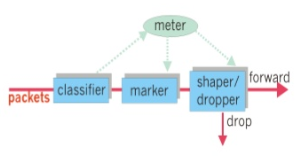
\includegraphics[width=0.5\textwidth]{img/edgerouter.PNG}
			\caption{Mecanismo de clasificación de paquetes del \textit{router} frontera. Fuente: Gsyc}
			\label{edgerouter}
		\end{figure}
	\item \textit{Router} núcleo de red: Estos \textit{routers} no realizan el encaminado de paquetes según los campos de origen y destino, sino que realizan el encaminado en función de la marca que trae ese paquete, tratando así a todos los paquetes de igual forma. En primer lugar se encolan los paquetes recibidos basándose en las marcas que pusieron los \textit{routers} frontera, acto seguido se les da preferencia a los paquetes cuya marca es \textit{in-profile}. Cada clase de tráfico (DSCP) está asociada a un tipo de salto (PHB) que determina el tipo de tratamiento que se le va a dar al paquete. Los PHB asociados al campos DSCP se detallan a continuación:
	\begin{itemize}
	    \item EF (\textit{Expedited Forwarding}): Esta clase de tráfico recibirá el suficiente ancho de banda para equiparar o igualar la tasa mínima configurada durante un intervalo de tiempo determinado.
	    \item VA (\textit{Voice Admit}): Similar a EF sólo que añade un mecanismo de control de admisión de tráfico.
	    \item AF (\textit{Assured Forwarding}): Existen cuatro clases diferentes con los que los paquetes son clasificados por el router frontera: AF1, AF2, AF3 y AF4. Cada clase ofrece una garantía y una prioridad diferente, siendo AF1 la clase más prioritaria y AF4 la menos prioritaria.
	    \item DF (\textit{Default Group}): Tráfico \textit{Best Effort}.
	    \item CS (\textit{Class Selector}): Ofrece retrocompatibilidad y permite definir prioridades.
	\end{itemize}
	\end{itemize}
	
	\subsubsection{MPLS}
		 MPLS (\textit{Mutiprotocol Label Switching}) es un mecanismo de transporte de datos que trabaja sobre la capa de red estableciendo enlaces vrtuales entre los nodos extremo de la red MPLS. El tráfico de datos es identificado mediante una etiqueta, evitando así la necesidad de utilizar la tablas de enrutamiento IP, y asociando a cada tráfico una etiqueta en particular que define la ruta destino. Además, este flujo puede tener asociados diferentes parámetros de QoS. Tal y como se muestra en la Figura \ref{mpls}, cada paquete tiene un camino predefinido; ese camino está definido mediante una etiqueta. Dichas etiquetas están distribuidas a los largo de la red mediante LDP (\textit{Label Distribution Protocol}). Este protocolo permite a los routers involucrados en la red, también denominados LDP \textit{peers}, intercambiar información de manera bidireccional sobre la red,  obteniendo así una base de datos LSP (\textit{Label-switched path}) sobre los diferentes caminos existentes y el tráfico existente en cada uno de ellos.
		 
		   \begin{figure}[H]
			\centering
			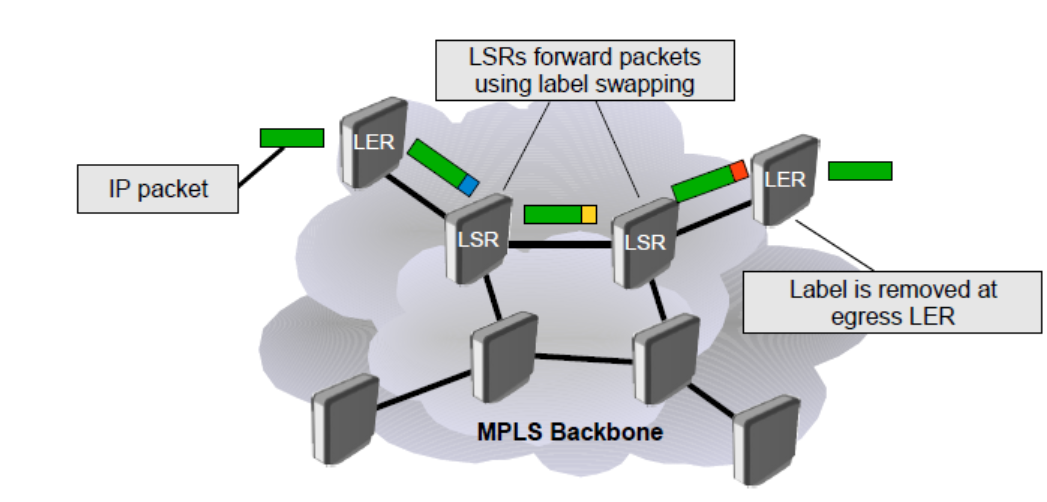
\includegraphics[width=0.5\textwidth]{img/mpls.PNG}
			\caption{Ejemplo de red MPLS. Fuente: Miro}
			\label{mpls}
		\end{figure}
		 El protocolo MPLS funciona sobre tecnologías de nivel 2 como ATM, Ethernet, etc... Aparte de poder configurar la red en función a QoS, es posible realizar configuraciones VPN (\textit{Virtual Private Network}) y TE (\textit{Traffic Engineering}). El datagrama MPLS mostrado en la Figura \ref{mplsData}, no es un datagrama IP convencional, si no que presenta alguna variación. Lo más destacado es el manejo de cabeceras, ya que los datagramas MPLS tienen una cabecera adicional que contiene que camino ha de tomar el paquete en cuestión. En algunos escenarios, es necesario el uso de más de una etiqueta debido a la complejidad de la red, a continuación se detallan algunos campos adicionales que son utilizados para el envío de paquetes:
		 \begin{itemize}
		    \item Etiqueta: Valor de la etiqueta MPLS.
		     \item TC (\textit{Traffic Class}): Es utilizado para identificar el tipo de QoS.
		     \item S (\textit{Bottom of Stack}): Se emplea para apilar etiquetas, cuando su valor es '1' quiere decir que es la última etiqueta.
		     \item TTL (\textit{Time To Live}): Misma funcionalidad que en otro tipo de redes, disminuye en una unidad cuando realiza un salto a lo largo de la red.
		 \end{itemize}
		 
		   \begin{figure}[H]
			\centering
			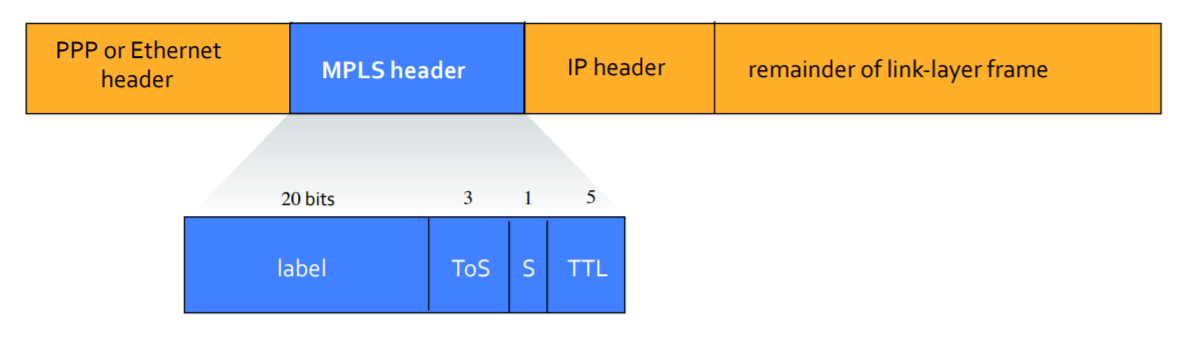
\includegraphics[width=0.5\textwidth]{img/datagramaMPLS.PNG}
			\caption{Representación de un datagrama MPLS. Fuente: ECCS}
			\label{mplsData}
		\end{figure}
		
		Al igual que los datagramas, la función y nomenclatura de los \textit{routers} involucrados en la red MPLS es diferente, ya que deben permitir reenviar paquetes utilizando las etiquetas MPLS. A continuación, se detallan los diferentes tipos de \textit{routers} involucrados en redes MPLS:
		\begin{itemize}
		    \item \textit{Ingress} LSR: \textit{Router} que se utiliza para acceder a la red MPLS interna. Es el encargado de añadir la primera etiqueta MPLS y realizar el reenvío correspondiente.
		    \item \textit{Intermediate} LSR: \textit{Router} ubicado en el medio de la red, debe recibir el paquete MPLS y reenviarlo al destino indicado por la etiqueta.
		    \item \textit{Egress} LSR: \textit{Router} ubicado al final de la red MPLS. Su función es desetiquetar el paquete y reenviarlo correctamente fuera de la red MPLS interna.
		\end{itemize}
		
	 La gestión de envío de los paquetes en los LSR se realiza en función de la etiqueta del paquete en cuestión y de la información contenida en la misma. En función de esa información, existen dos formas de recibir el paquete: por interfaz o por \textit{router}. Por un lado, si se realiza un reenvío por \textit{router} únicamente se reenvía utilizando la información de la etiqueta. Por otro lado, si utilizamos el reenvío mediante interfaz se utiliza la información existente en la interfaz del \textit{router} y la información existente en la etiqueta. En este último, cada \textit{router} puede definir su propio ámbito de etiquetas.\\
	 Aparte del uso de estas técnicas, los LSR también utilizan tablas adicionales para la gestión de reenvío de paquetes; a continuación se detallan dichas tablas:
	 \begin{itemize}
	     \item NHLFE (\textit{Next Hop Label Fordwarding Entry}): Gestiona las etiquetas de salida.
	     \item ILM (\textit{Incoming Label Map}): relaciona la etiqueta con la entrada correspondiente en la tabla NHLFE.
	     \item FTN (\textit{FEC-To-NLHFE Map}): Identifica los parámetros de una clase con la entrada correspondiente en la tabla NHLFE. Esta tabla es utilizada cuando no existe etiqueta.
	 \end{itemize}
	 Los \textit{routers} intermedios (\textit{Intermediate} LSR) deben estar sincronizados y orquestados en cuanto a las etiquetas utilizadas y protocolos durante el reenvío de paquetes; para este cometido debemos definir un protocolo que permita distribuir y realizar un control del etiquetado existente en la red. A continuación se definen los protocolos utilizados para este cometido:
	 \begin{itemize}
	     \item \textit{Label Distribution Protocol} (LDP): Este protocolo estable sesiones TCP entre los LSR involucrados para intercambiar las etiquetas que utilizarán durante el intercambio de paquetes.
	     \item \textit{Resource Reservation Protocol - Traffic Engeniering} (RSVP-TE): Es un protocolo similar a LDP, salvo que permite configurar los diferentes LSPs (\textit{Label Switch Path}) de forma explícita, ya sea total o parcial. Se define LSP como el camino unidireccional que contiene la secuencia de LSR que reenvían un paquete. Al igual que es posible establecer un LSP de forma explícita este protocolo permite añadir restricciones al mismo.
	 \end{itemize}
	 
	 \subsubsection{MPLS-TE}
	 MPLS-TE es una variación frente a MPLS que mejora el encaminamiento de paquetes mediante la implementación de LDPs y distribución de etiquetas a través de LDP. La diferencia con MPLS, y principal característica de TE, es que nos permite realizar conexiones entre nodos finales dentro de la propia red, tal y como muestra la Figura \ref{mplste}.\\
	 MPLS-TE utiliza el protocolo RSVP-TE para definir enlaces internos que son denominados túneles y restringen el uso de los recursos compartidos de la red a los circuitos virtuales que la forman, creando así una protección mutua entre ellos. Como consecuencia de esto, la distribución del ancho de banda es igual o inferior al total disponible. Al igual que en MPLS es posible configurar los diferentes túneles en función de las propiedades de la red y las interfaces de los LSR involucrados.
	 
	 \begin{figure}[H]
			\centering
			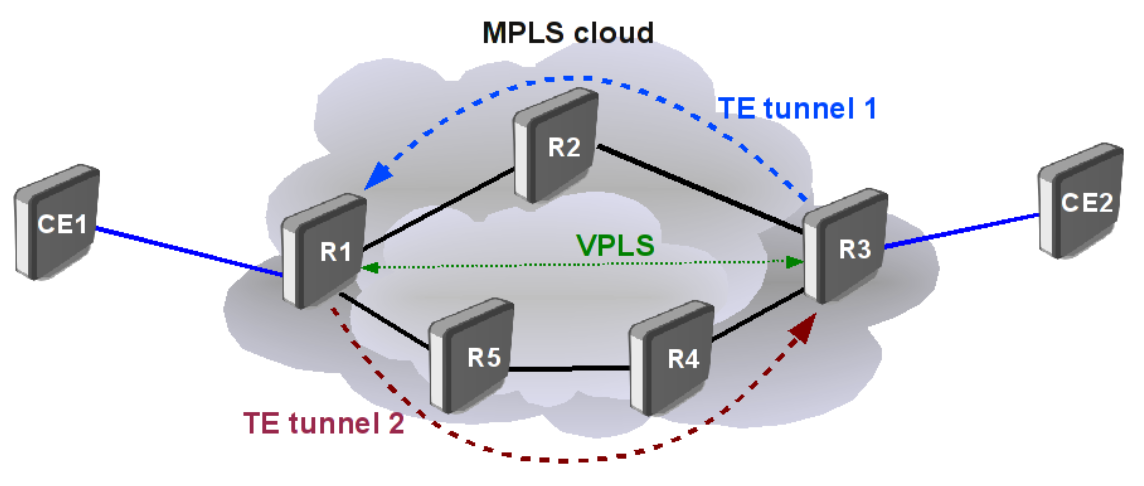
\includegraphics[width=0.5\textwidth]{img/mplste.PNG}
			\caption{Ejemplo de red MPLS-TE. Fuente: MikroTik}
			\label{mplste}
		\end{figure}
		

	\section{Gestión de redes}
Para que una red operativa sea mantenible de forma sostenible con una cantidad razonable de recursos, es preciso disponer de alguna clase de sistema de gestión de red. Su función es la monitorización y el control de la red de forma eficaz y eficiente. Un sistema de gestión de red debe tener una imagen de lo que sucede en la red lo más precisa posible y en tiempo real, de manera que si hay algún problema de recursos, alguna falla, algún problema de configuración o de seguridad, pueden detectarse de forma rápida para poner medidas correctoras en marcha y evitar (o acortar) situaciones de indisponibilidad de la red y de los servicios que ésta soporta; así mismo, la función de control de un sistema de gestión de red permite actuar sobre la red desde un sistema, al más alto nivel posible, para minimizar los recursos con los que se tiene que implementar cualquier actuación sobre la misma. \\

En este proyecto era preciso identificar una herramienta sencilla y no costosa para la gestión de la red, pues estratégicamente es fundamental poder gestionar una red tan dispersa geográficamente y en la que cualquier intervención de operación y mantenimiento tiene un elevado coste en desplazamientos, plazos y recursos humanos; sin embargo, en el proyecto inicial no estaba prevista una partida presupuestaria para la implantación de un sistema de gestión de red. Afortunadamente, existen varias herramientas muy maduras y de gran calidad de \textit{software} libre para gestión de redes. Las que se han identificado y valorado como alternativas para este proyecto son las siguientes:
	  
	\begin{itemize}
		\item Nagios Core \cite{Nagios} es un \textit{software} diseñado y desarrollado por la empresa Nagios. Permite monitorizar vía web cualquier infraestructura y dispositivo red, estableciendo un conjunto de reglas basadas en servicios y alertas reportando información sobre el funcionamiento de la red.\\
		Nagios Core ofrece gran variedad de servicios y funcionalidades respecto a la monitorización, siendo capaz de monitorizar servicios red (HTTP, SNMP, POP3, etc...) y recursos de los dispositivos (carga de CPU, temperatura, espacio libre, etc...). Igualmente, existe la opción de autoconfigurar y desarrollar nuestros propios servicios y no sólo utilizar los predefinidos por el fabricante (que aparecen por defecto). También existe la posibilidad de generar notificaciones sobre cualquier servicio, y éstas pueden ser enviadas vía email (u otro método que defina el usuario). Para una configuración personalizada no hacen falta librerías adicionales, ya que la versión Core incluye todas las funcionalidades básicas para la gestión y monitorización de redes. No obstante, se pueden incluir otras funcionalidades como representación de gráficos en un \textit{Dashboard}, exportación de configuraciones o utilización de proveedor de correo externo al de la propia herramienta. Todo esto podremos hacerlo mediante la adicción de \textit{plugins} al Core.
		
		\item Zabbix \cite{Zabbix} es un \textit{software} íntegramente libre desarrollado por Zaabix SIA. Este \textit{software} nos permite monitorizar numerosos parámetros de nuestra red, bien sean servicios (HTTP, SNMP, SSH, etc..) o bien sean parámetros de los dispositivos (uso de CPU, porcentaje uso de CPU, temperatura, etc...) referidos a los servicios y estado de los dispositivos que la componen. Para ello, Zabbix utiliza un sistema de notificaciones configurables, las cuales pueden enviarse vía email (utilizando cualquier proveedor de correo). Dichas notificaciones nos informarán sobre los sucesos que están ocurriendo sobre los dispositivos red y los servicios configurados.\\
		En orden con lo anterior, Zabbix permite editar y configurar diferentes tipos de notificaciones y alertas sin necesidad de añadir nada a la herramienta. Además de esto, el reporte de datos es periódico y no sólo de manera numérica sino de forma gráfica (dichas gráficas también pueden ser configurables). Del mismo modo, existe la posibilidad de almacenar todo los datos reportados procedente de los dispositivos que forman la red en bases de datos (MySQL, SQLite, PostgreSQL u Oracle).
		
		\item Pandora OpenSource \cite{Pandora} es un \textit{software} de gestión y monitorización, desarrollado por la empresa Pandora FMS Enterprise, que proporciona una solución capaz de monitorizar cualquier infraestructura de red asegurando que todos los elementos de la red estén funcionando bajo los criterios de operación establecidos. Esto es debido a la información procedente de los dispositivos de la red al realizarse pruebas sobre ellos, ya sea de manera remota o mediante un agente. \\
		La versión libre de este software permite monitorizar y gestionar parámetros referentes a los servicios de red estándar TCP/IP y valores relacionados con el hardware de los equipos gracias a un sistema de eventos. Este sistema obtiene la información al producirse cualquier evento en la red. Al basarse en dicha funcionalidad, el usuario puede validar los eventos y agruparlos según la distribución de la red. Debido a esto el software utiliza una monitorización combinada en grupos, lo que quiere decir que, según el grupo en el que se encuentre un dispositivo, sus alertas y su configuración de servicios serán diferentes al resto.\\
	\end{itemize}
	
	Una vez introducidos diferentes sistemas de gestión de red valorados, vamos a analizar cual de ellos encaja mejor en el marco de nuestro proyecto según las diferentes limitaciones y requisitos.\\
	
	En primer lugar, nuestro \textit{software} debe ser capaz de monitorizar todos los requisitos mínimos para garantizar un cierto nivel de QoS. Además de esto es conveniente que exista cierta flexibilidad a la hora de modificar y añadir notificaciones en los diferentes equipos, así como la posibilidad de recibir y enviar dichas notificaciones al personal de operación y mantenimiento de red mediante e-mail, o cualquier método similar. Del mismo modo, el \textit{software} debe tener una integración sencilla sobre nuestra infraestructura de red.\\
	
	En segundo lugar, la obtención y representación de datos de forma dinámica es una parte importante que la herramienta ha de tener. Lo deseable es que la infraestructura de red sea autogestionable y plenamente monitorizable por el propio \textit{software}, es decir, tratar de que cualquier servicio y parámetro pueda ser representado de manera concreta para otorgar al usuario la información adecuada para interactuar, si fuera necesario, con la red.\\
	
	En tercer lugar, nuestro \textit{software} ha de ser flexible en cuanto a escalabilidad de dispositivos y configuración de notificaciones, puesto que nuestra red es extensa y heteréogenea en cuanto al número de equipos y su uso. Otro requisito a tener en cuenta es que debe cumplir con un sistema de negocio viable, ya que el proyecto tiene limitada la inversión económica y es muy deseable utilizar un software cuya prestación cubra los requisitos sin incrementar los costes de despliegue y de operación.\\
	
	Teniendo en cuenta todo lo comentado anteriormente, la solución propuesta para el proyecto es Zabbix.	Zabbix permite una fácil integración y monitorización de la red, permitiendo al usuario administrar los dispositivos y configurar los servicios de manera sencilla sin excesiva complejidad. Gracias a su interfaz gráfica podemos obtener en todo momento una representacion en tiempo real del estado de los dispositivos, así como de los requisitos pertenecientes al QoS. Dichos datos pueden ser almacenados en bases de datos y exportados a ficheros.\\
	Por un lado, Zabbix no sólo permite al usuario definir dispositivos, sino que existe la posibilidad agruparlos en diferentes categorías, otorgando la opción de realizar una gestión individualizada o colectiva, según desee el usuario. Por otro lado, se pueden crear servicios mediante un fichero XML y vincularlo con el dispositivo deseado,  configurando alertas y notificaciones personalizadas. Con la revisión que se ha podido hacer en el marco de este proyecto, se ha considerado que las otras alternativas podían llegar a cubrir igualmente todas las necesidades, especialmente Nagios, pero con una curva de aprendizaje y un esfuerzo de configuración y de operación mayores, lo que ha inclinado la balanza hacia Zabbix.
	
	\chapter{Metodología}
\label{cap:metodologia}
En este capítulo se explicará todo lo relacionado con la metodología utilizada en este Trabajo Fin de Grado. Con el objetivo de encontrar una solución sostenible, flexible en términos de negocio y que sea capaz de amoldarse a las especificaciones y criterios del proyecto.\\\\

En primer lugar, se realizará una introducción a los equipos utilizados en el proyecto tanto a nivel software como hardware. Se detallarán las especificaciones técnicas y características de los equipos, así como su motivación para ser usados en este proyecto. De la misma manera se explicará el funcionamiento del software de configuración disponible en los equipos.\\\\

En segundo lugar, se realizarán pruebas a nivel de laboratorio utilizando configuraciones similares a las utilizadas en el marco del proyecto Napo. Siguiendo un escenario base de laboratorio, se analizará el rendimiento de los equipos a nivel de red, utilizando para ello herramientas cuya funcionalidad será la inyección de tráfico simulado. De forma paralela se utilizará la solución propuesta en el capítulo \ref{cap:marco_teorico} para realizar la gestión y monitorización de redes sobre el escenario red disponible en laboratorio.

\section{Equipos propuestos}
Con el objeto de seleccionar aquellos equipos que mejor rendimiento y prestaciones ofrezcan al proyecto, se ha establecido una comparativa y estudio entre diferentes propuestas. Dichas propuestas no sólo deben adaptarse y cumplir a los requerimientos técnicos del proyecto, si no que también deben mostrar un rendimiento adecuado al coste establecido por el proyecto.\\\\

Para ello se ha establecido un protocolo de pruebas que nos ofrecerá el rendimiento de los equipos sobre pruebas realizadas en campo, gracias a la aportación de la PUCP. Dichas pruebas determinarán qué equipos son los finalmente seleccionados como solución del proyecto. A continuación, se procede a detallar cada uno de los equipos involucrados en este estudio y la comparativa entre ellos.

\subsection{Equipos Ubiquiti}
Los equipos pertenecientes a la empresa estadounidense Ubiquiti Networks \cite{Ubiquiti}, son exportados y utilizados a lo largo de todo el mundo en lo que a comuniaciones inalámbricas se refiere, convirtiendo así a la empresa en un referente mundial. Esta empresa se dedica principalmente al desarrollo y comercialización de dispositivos para redes inalámbricas, ya sean de larga o corta distancia. \\\\

Los equipos desarrollados por la empresa se caracterizan por su alto rendimiento, su bajo coste y su alta eficiencia energética, cmpliendo así con los requisitos mínimos establecidos en el proyecto Napo. En el marco del proyecto los equipos Ubiquiti AirFiber AF-5X y PowerBeam 5AC-620, los cuáles se detallarán a continuación, han sido propuestos como solución. De igual forma, se ha detallado el \textit{software} de gestión de los equipos Ubiquiti, que en el caso de ambos funciona de idéntica forma.

\subsubsection{AirFiber AF-5X}
Los dispositivos AF-5x están diseñados con una carcasa de silicona que recubre la placa empotrada que forma el equipo, tal y como se muestra en la figura \ref{af_5x}, el diseño sencillo de los equipos y sus conexiones salientes hacen de él un equipo muy versátil y flexible a la hora de ser integrado con otros componentes, como por ejemplo una antena o un sistema empotrado sobre una torre. Aparte de su flexibilidad a nivel físico, también ofrece gran versatilidad en su comportamiento, permitiendo así utilizar este equipo en diferentes roles según requiera la arquitectura diseñada, ya sea bien como estación base, o como un repetidor. De igual forma, su sistema está diseñado para ofrecer el máximo rendimiento de la transmisión mediante la reducción de señales interferentes y habilitando la posibilidad de utilizar constelaciones mayores para obtener un mayor \textit{throughput}.

\begin{figure}[H]
		\centering
		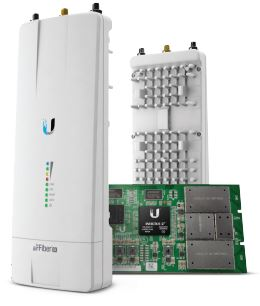
\includegraphics[width=5cm,height=5cm]{img/af_5x.JPG}
		\caption{Dispositivo AF-5X}
		\label{af_5x}
	\end{figure}

 Los dispositivos radio de esta familia, utilizan la banda de 5 GHzs como frecuencia operacional y no sólo eso, si no que además este modelo abarca todo el espectro radioeléctrico en el rango de 5 GHzs, tanto las bandas licenciadas como las que no lo son. Aparte de esto, estos equipos permiten ajustar el ancho de banda operacional, en el caso del modelo AF-5X de 10 a 50 MHzs, en intervalos de 10 MHzs otorgando mayor flexibilidad a la configuración de canales de subida y de bajada. Además de esto, los equipos permiten ajustar los canales de transmisión y recepción evitando así que existan interferencias en los canales seleccionados.
	
\subsubsection{PowerBeam 5AC-620}
La familia de equipos PowerBeam, independientemente del modelo, se caracteriza por su estructura y diseño, ya que tal y como se muestra en la figura \ref{powerBeam} el dispositivo radio está integrado junto a la estructura de la parabólica, proporcionando así un mejor acople ya que se evitan las pérdidas con cable. Además esta característica en el diseño, los equipos PowerBeam cuentan con la tecnologías AirMAX AC desarrollada por Ubiquiti que permite focalizar la comunicación en una única dirección ofreciendo así robustez frente a interferencias filtrando el ruido no deseado.

\begin{figure}[H]
		\centering
		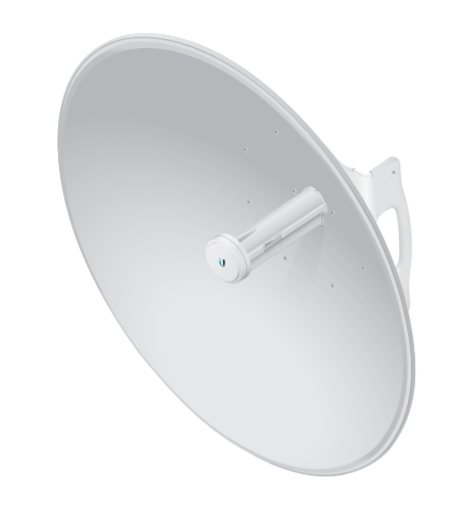
\includegraphics[width=5cm,height=5cm]{img/powerbeam.PNG}
		\caption{Dispositivo PowerBeam 5AC-620}
		\label{powerBeam}
\end{figure}

Otra característica importante de estos equipos es cómo permiten a los usuarios utilizar los enlaces para subida y descarga de datos. En este caso, la tecnologías AirMAX utiliza el protocolo de acceso al medio TDMA pero con una modificación desarrollada por Ubiquiti, ilustrado en la figura \ref{tdma_ac}. Esta modificación consiste en asignar previamente \textit{slots} de tiempo a los usuarios mediante un punto de acceso inteligente integrado en el propio dispositivo, esto permite minimizar problemas de colisión cómo el problema del nodo escondido y aumentar el rendimiento del equipo llegando a obtener tasas mayores a 450 Mbps mientras que los equipos sin dicha tecnologías se mantienen en el umbral de 150 Mbps.
	
\begin{figure}[H]
		\centering
		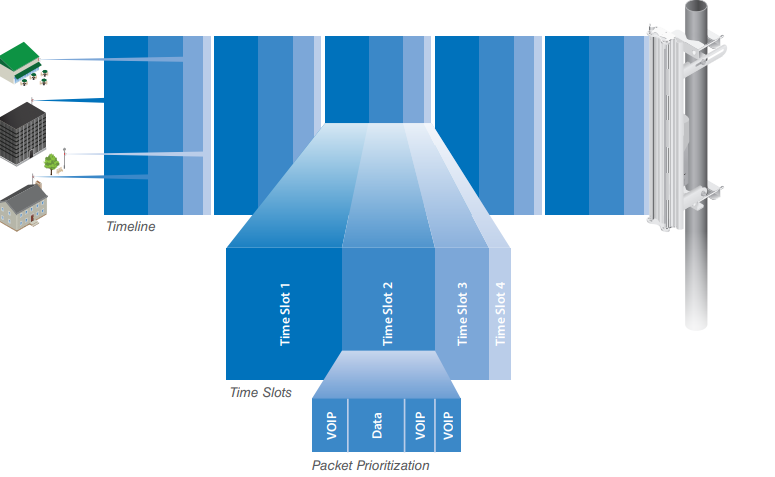
\includegraphics[width=0.5\textwidth]{img/tdma_ac.PNG}
		\caption{Protocolo TDMA con tecnologías AirMAX AC}
		\label{tdma_ac}
\end{figure}
	
\subsection{Software}
Los equipos propietarios de la marca Ubiquiti utilizan un \textit{software} propietario que permite controlar y configurar los equipos. Aunque no esté en su versión final, el programa Ubiquiti Network Management System (UNMS) otorga al usuario un control absoluto sobre los dispositivos que conforman la red, y una serie de aplicaciones internas para obtener una correcta parametrización del rendimiento de los equipos. Tal y como se muestra en la figura \ref{unms} podemos ver como la pantalla principal del \textit{software} muestra diferentes tipos de configuración, paneles de interacción con el usuario, así como diferentes pestañas en las cuales se muestran datos a tiempo real del rendimiento de los equipos. 

\begin{figure}[H]
		\centering
		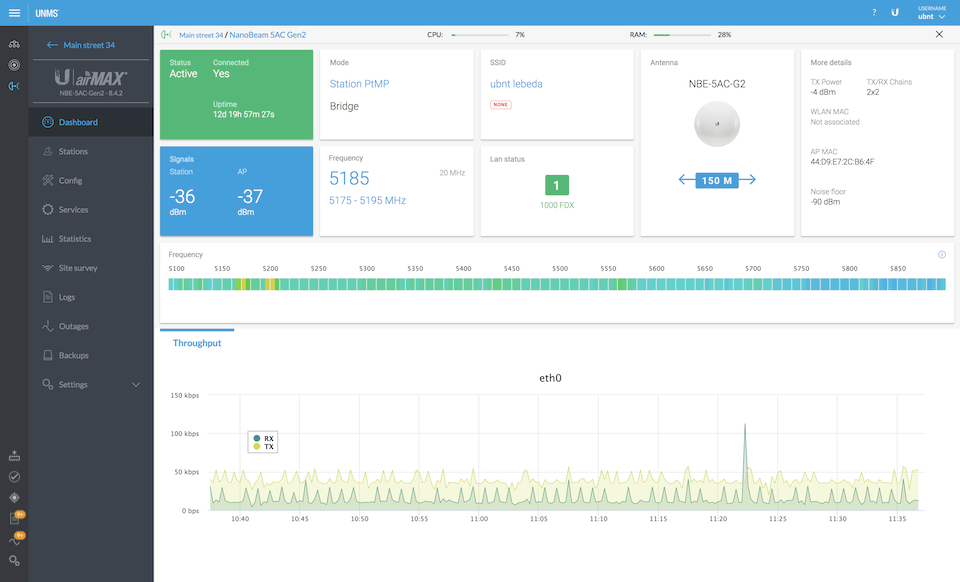
\includegraphics[width=0.5\textwidth]{img/unms.png}
		\caption{Pantalla principal UNMS}
		\label{unms}
	\end{figure}
	
Aparte de las funcionalidades antes comentadas, UNMS ofrece la posibilidad de obtener datos referentes al rendimiento de los equipos en lo que a parametrización de red respecta, es decir, todo lo relacionado con tráfico entrante y saliente de la red, niveles de recepción de señal, etc... Dichos parámetros pueden obtenerse utilizando una apicación interna que la propia herramienta tiene integrada consigo.

\subsection{Equipos VNL: RM-MAX}
Los equipos RM-MAX son dispositivos que pertenecen a las placas inalámbricas que fabrica y comercializada la empresa VNL \cite{VNL}. Fundada en 2004, VNL se dedica al desarrollo e implementación de equipos para infraestructuras de telecomunicaciones punto a punto. Aunque su principal enfoque estratégico sea en aplicaciones militares y civiles, actualmente existe una creciente demanda de uso de estos equipos en zonas rurales de países en vías de desarrollo, como por ejemplo India, Nepal o Indonesia.\\\\

Los equipos RM-MAX  utilizan OFDM como protocolo de acceso al medio, pero este procotocolo no es el nativo, es decir, es una variante propietaria de VNL que permite mantener las conexiones existentes de forma prolongada evitando caídas con la parte \textit{core} de la red. De igual forma, los equipos permiten un control absoluto sobre las transmisiones existentes en la red, consiguiendo así una reducción en costes importante evitando el uso de líneas cableadas. Otro factor a tener en cuenta, es que dichos equipos están fabricados y desarrollados bajo la metodología \textit{Plug and Play}, lo que quiere decir que su instalación y configuración se realiza forma rápida y sencilla.

\subsubsection{Hardware}
Los equipos RM-MAX escogidos como solución de este proyecto, son capaces de cubrir una distancia superior a los 100 Km incluyendo diferentes configuraciones según la frecuencia que deseemos usar. Tal y como se muestra en la figura \ref{rm_max}, la antena está integrada en una placa cuyo recubrimiento metálico hace que este equipo sea robusto frente a situaciones climatólogicas adversas. De igual forma dichos equipos están dotados de diferentes modos de funcionamiento, lo que permite mayor versatilidad a lo hora de configurar un tipo determinado de infraestructura, de igual forma estos equipos admiten diferentes modos de actuación, ya sea bien como estación base o como \textit{bridge}.

\begin{figure}[H]
		\centering
		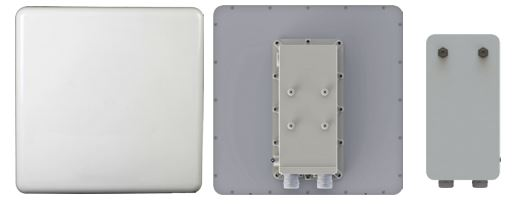
\includegraphics[width=0.5\textwidth]{img/rm_max.JPG}
		\caption{Dispositivo RM-MAX}
		\label{rm_max}
	\end{figure}
	
\subsubsection{Software}
Los equipos VNL utilizan como \textit{software} de gestión y configuración el \textit{Radio Modem Management}, dicho programa es propietario de VNL y muestra un aspecto similar al que se muestra en la figura \ref{vnl_rm}. Dicha aplicación permite configurar de manera sencilla los parámetros de red deseables en cuanto a configuración se refiere, obteniendo así un escenario versátil y fácilmente gestionable. De igual forma, la aplicación nos permite configurar perfiles de seguridad y administración para atribuir mayor robustez a la red configurada. 

\begin{figure}[H]
		\centering
		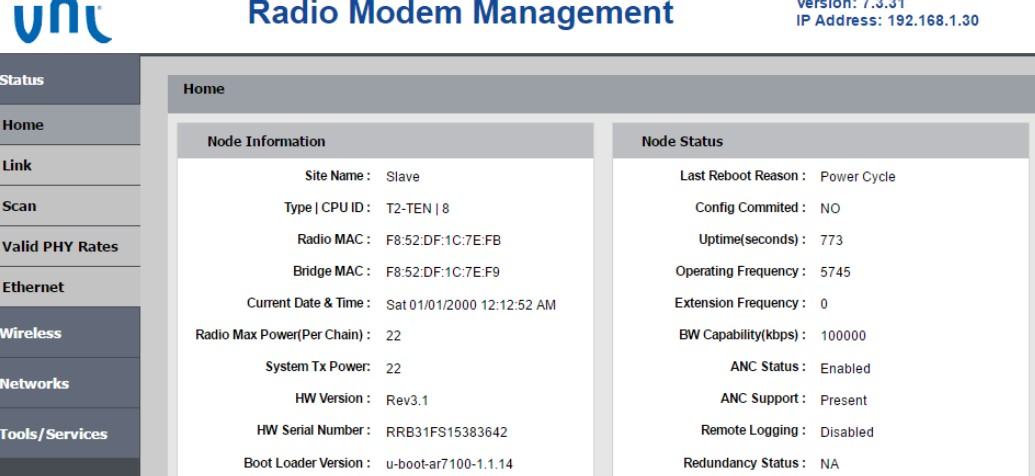
\includegraphics[width=0.5\textwidth]{img/vnl_rm.jpg}
		\caption{Pantalla principal \textit{Radio Modem Management}}
		\label{vnl_rm}
	\end{figure}

Por otra parte, la aplicación ofrece la posibilidad de configurar páginas de entrada por el usuario, permitiendo así una mayor personalización de la herramienta en función del perfil del usuario. Esta funcionalidad permite al usuario obtener datos en tiempo real del estado y actuación de los equipos involucrados en la red. 

\subsection{Equipos Mikrotik: NetMetal 5}
Los equipos NetMetal 5 son dispositivos pertenecientes a la familia de RouterBOARDS diseñadas y comercializadas por la empresa MikroTik \cite{Mikrotik}. Dicha empresa, se dedica al desarrollo de sistemas hardware y software inalámbricos en variedad de países a lo largo del mundo. El uso de sus equipos está extendido a nivel mundial debido a su bajo coste y a su alto rendimiento en sistemas de telecomunicaciones inalámbricas.
	\subsubsection{Hardware}
	Los equipos NetMetal disponen de un procesador MIPSBE que opera a 720MHzs y un recubrimiento hecho de aluminio y metal, su aspecto se muestra en la figura \ref{equipo}, lo que permite un gran rendimiento en zonas donde existen condiciones climatológicas adversas. El equipo está formado por tres puertos cuya funcionalidad es: la conexión de antenas externas en dos de ellos (permitiendo el uso de MIMO), y un terminal POE en el que se encuentran las entradas para la conexión mediante ethernet y la fuente de alimentación.
	\begin{figure}[H]
		\centering
		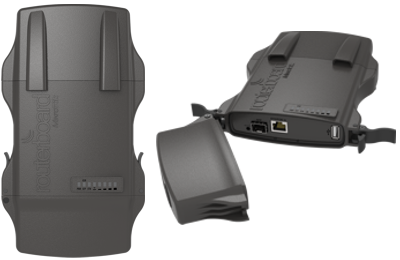
\includegraphics[width=0.5\textwidth]{img/netMetal5.png}
		\caption{Dispositivo NetMetal 5}
		\label{equipo}
	\end{figure}
	Existe una variante en los equipos, el cúal en vez de proporcionar tres entradas para antenas externas únicamente proporciona dos entradas.
	Los equipos NetMetal 5 son capaces de alcanzar altas tasas de transmisión en comunicaciones inalámbricas de larga distancia, gracias al uso del estándar 802.11ac y su eficiencia en cuánto al uso de los canales de 20/40/80 MHzs. Este hecho añadido a su robustez hacen de los equipos una elección idónea para el contexto del proyecto.\\
	Para llevar a cabo este Trabajo Fin de Grado, se han utilizados dos equipos NetMetal 5 como escenario de laboratorio.
	\subsubsection{Software}
	El sistema operativo que utilizan los equipos es RouterOS, propietario de MikroTik. Dicha distribución nos permite acceder al dispositivo de manera sencilla y configurar el equipo acorde al escenario requerido. Además de realizar configuraciones en cuánto a los parámetros deseados, el sistema operativo ofrece herramientas para la realización de pruebas a diferentes niveles de conectividad entre equipos. Los datos obtenidos, pueden ser procesados y representados de forma gráfica en tablas, diagramas y ficheros de texto. Independientemente de un formato u otro existe la posibilidad de exportar estos datos.\\\\
	
	Así mismo los equipos permiten exportar e importar las configuraciones realizadas siendo esto de gran utilidad a la hora de replicar una configuración en diferentes equipos. Por último este sistema operativo es compatible con cualquier distribución para PC, ofrece más de una variante para utilizar y configurar los equipos, ya sea mediante línea de comandos, interfaz web o utilizando la aplicación WinBox que se detalla a continuación.\\\\
	
	WinBox permite conectar los equipos de manera rápida y sencilla a través de su dirección IP o MAC, tal y como se muestra la siguiente figura \ref{inicioWinBox}. La configuración de usuario e IP vienen predeterminadas por el fabricante.\\
	Una vez logueado dentro del equipo, tal y como se muestra en la figura \ref{mainWinBox}, aparecen multitud de paneles y menús los cuáles nos servirán para configurar los equipos, ya sea en cuestiones de seguridad, creación de redes, configuración de interfaces, etc... Aparte de modificar la configuración que se establece predeterminada, WinBox ofrece la posibilidad de realizar mediciones para determinar el rendimiento de los equipos, como por ejemplo el número de paquetes envíado durante una transmisión.
		\begin{figure}[H]
			\centering
			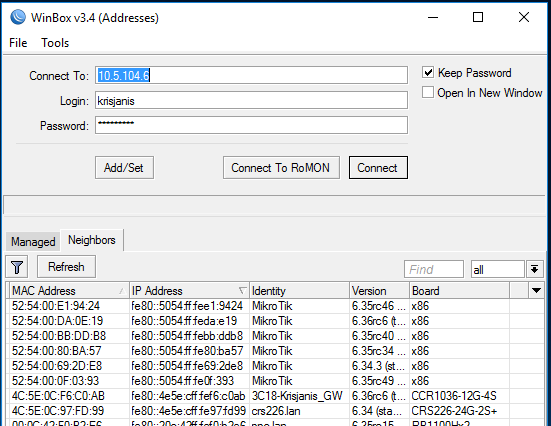
\includegraphics[width=0.7\textwidth]{img/winbox_loader.png}
			\caption{Pantalla loging en WinBox}
			\label{inicioWinBox}
		\end{figure}
		\begin{figure}[H]
			\centering
			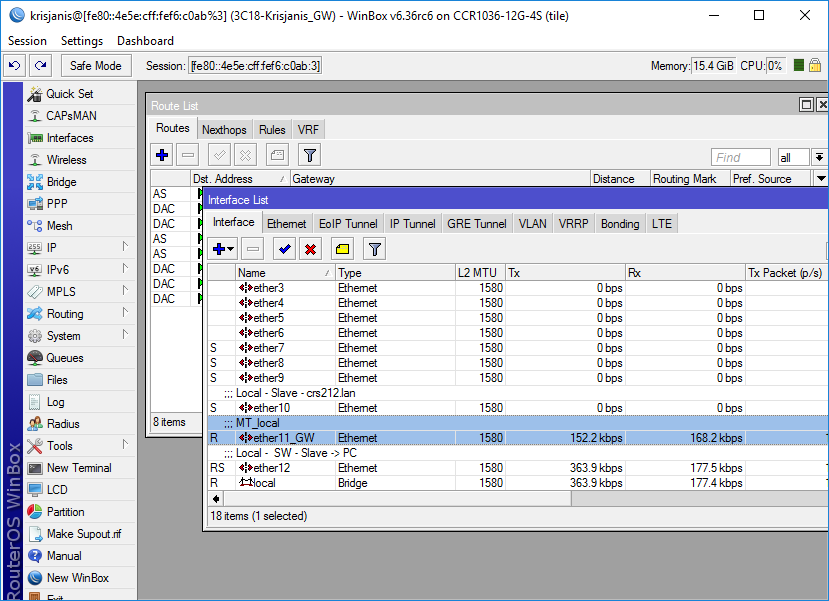
\includegraphics[width=0.7\textwidth]{img/winbox.png}
			\caption{Pantalla principal en WinBox}
			\label{mainWinBox}
		\end{figure}
		Al igual que la herramienta web, WinBox ofrece la posibilidad de utilizar una terminal compatible con el equipo y sistema operativo RouterOS. Dicha funcionalidad permite introducir y modificar las configuraciones existentes en los dispositivos, así cómo visualización de parámetros y realización de pruebas utilizando las herramientas integradas que posee el sistema operativo.
		
\section{Comparación entre equipos}	
Antes de proceder a comparar los equipos detallados anteriormente, debemos primero explicar el protocolo de pruebas que se ha elaborado con la colaboración de los compañeros involucrados pertenecientes a la PUCP. Dicho protocolo nos servirá para valorar y evaluar las prestaciones de cada uno de los equipos de forma individual y establecer una comparativa, con el fin de obtener una solución lo más viable y factible posible en lo que al marco del proyecto se refiere. \\\\

 El protocolo de pruebas diseñado en colaboración con la PUCP no sólo implica realizar pruebas de campo con los equipos, si no que se realizarán simulaciones parametrizadas en RadioMobile a modo complementario para decidir cúal es el equipo que más se adapta a las condiciones del proyecto. Las pruebas de campo conllevarán la configuración de un enlace punto a punto en las instalaciones disponibles para dicho efecto de la PUCP. Una vez configurado el enlace, se realizarán pruebas de conectividad utilizando programas para inyectar tráfico y se examinarán los valores obtenidos. De forma simultánea, se registrarán los valores energéticos proporcionados por los equipos durante las pruebas para contrastar su eficiencia energética.\\\\
 
 Las pruebas realizadas por la PUCP han sido llevadas a cabo en diferentes emplazamientos, ubicados en Iquitos-Mazán para el caso de los equipos Net Metal 5 y RM-MAX, y por otro lado para los equipos Ubiquiti en los emplazamientos encontrados en Pachatutec (Ventanilla) y San Miguel. No obstante, las características de los emplezamientos mencionados y sus perfiles geográficos son muy parejos, por lo tanto sí que nos sirven para realizar nuestro análisis. De igual forma, este estudio se ha tenido que realizar de forma interrumpida, es decir primero una pareja de equipos y después la otra, debido a las disponibilidad de los emplazamientos y equipos.\\
 La configuración de ambos escenarios sigue un esquema como el mostrado en la figura \ref{pruebasPUCP}, el cúal está compuesto por torres metálicas sobre las cuáles se encuentran antenas de igual ganancia que las existentes en las instalaciones del río Napo.
 
 
 \begin{figure}[H]
			\centering
			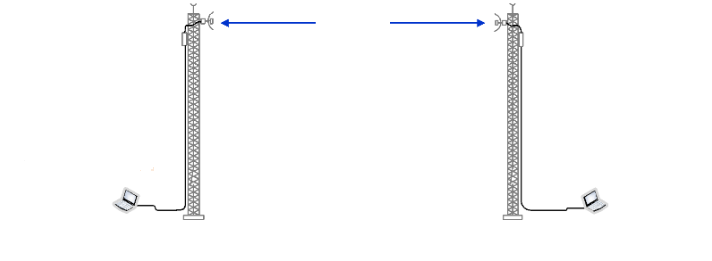
\includegraphics[width=0.7\textwidth]{img/escenario_pruebas.png}
			\caption{Escenario de pruebas propuesto PUCP}
			\label{pruebasPUCP}
\end{figure}
 
\section{Configuración y diseño de la red}
Antes de realizar el montaje del escenario y realización de pruebas en laboratorio, debemos realizar un diseño y estudio sobre la red. Dicho análisis nos permitirá conocer de forma más detalla los diferentes factores que pueden comprometer la viabilidad de los diferentes enlaces que componen la red, y así ajustar la configuración de los equipos a dichos factores para garantizar el objetivo y requisitos predefinidos en el proyecto.\\\\

Tras la conlcusión de la parte correspondiente al estudio y diseño de la red, realizaremos nuestras simulaciones a nivel de laboratorio. El objetivo de esto, será establecer una comparación con los resultados obtenidos en la fase de estudio, para ello dispondremos de los equipos NetMetal 5 y ordenadores cuya distribución será Linux. Ya que los sistemas operativos pertenecientes a dicha distribución, otorgan facilidades a la hora de instalar y manejar los programas necesarios para la realización de pruebas. Las pruebas llevadas a cabo determinarán el rendimiento que ofrecen los equipos NetMetal 5 en lo que a conectividad y parámetros de calidad se refiere.

\subsection{Estudio previo} 
	En esta sección procederemos a realizar un estudio de forma cuantitativa con el objetivo de conocer cual sería el \textit{throughput} obtenido de forma teórica, por cada uno de los radioenlaces que forman la red del Napo. Para ello utilizaremos los valores empirícos obtenidos en el artículo \cite{simo2014assessing} recogidos en la tabla número 7,  pertenecientes al uso del protocolo NV2.\\\\
	
	Por una parte, los valores presentes en dicha tabla corresponden a medidas de capacidad en radioenlace para una distancia de 0 Km (medidas en laboratorio) y una distancia de 30 Km, las medidas fueron llevadas a cabo desde la modulación MCS0 hasta MCS15 para la mayoría de casos, salvo en las mediciones de 30 Km, qué para valores superiores a MCS11 no se pudieron realizar pruebas empirícas. No obstante, sólo nos apoyaremos y tomaremos como referencia los valores comprendidos entre la modulación MCS8 y MCS11 ya que son las modulaciones destinadas para el uso de MIMO. \\
	Por otra parte, dichas medidas corresponden a la utilización de 20 Mhz como ancho de banda, para poder establecer una relación con el ancho de banda utilizado en el proyecto se procederá a duplicar los valores obtenidos a 20 Mhz. Obteniendo así un aproximación de los valores teóricos que deberían ser obtenidos de forma empiríca para un ancho de banda de 40 Mhz; una vez concluida la parte teórica se contrastarán dichos valores con los obtenidos en laboratorio y se procederá a realizar un análisis más exhaustivo.\\\\
	
	Para poder llevar a cabo el estudio teórico, se han recogido los valores antes mencionados y se han organizado en pares de coordenadas obteniendo un conjunto de datos que establecen una relación entre: la distancia, \textit{throughput}, y el valor de la modulación MCS utilizado. Una vez acondicionados los datos se ha proyectado una recta lineal entre los puntos pertenecientes a cada MCS respecto a las coordenadas base de 0 Km y 30 Km, con el objetivo de obtener una recta que pase por todos los puntos de interés de nuestra red, tal y como muestra la figura \ref{rectaspendiente}, permitiendo establecer así una aproximación teórica de la capacidad del enlace en función de la distancia.\\\\
	
	De forma paralela, en base a la obtención de las rectas respecto a cada MCS hemos podido realizar una estimación de la capacidad teórica que debería de existir para cada radioenlace, dicha estimación se muestra en la figura \ref{valoresmbps}. Para llevar a cabo todo el estudio teórico y todo el desarrollo comentado anteriormente, se ha utilizado el script \ref{lst:script}, que está desarrollado en el lenguaje de programación Python, ya que permite la integración de módulos y librerías de análisis matemático de forma sencilla.
	
	\begin{figure}[H]
		\centering
		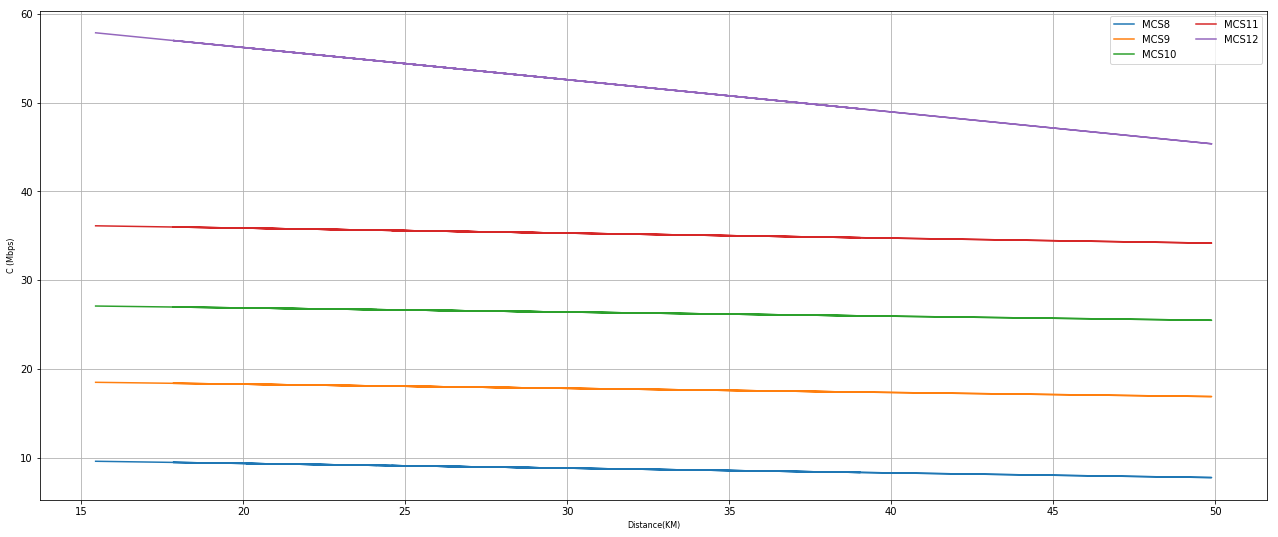
\includegraphics[width=0.7\textwidth]{img/rectas.png}
		\caption{Rectas lineales utilizando valores de 0 Km y 30 Km como coordenadas base}
		\label{rectaspendiente}
	\end{figure}
	
	\begin{figure}[H]
		\centering
		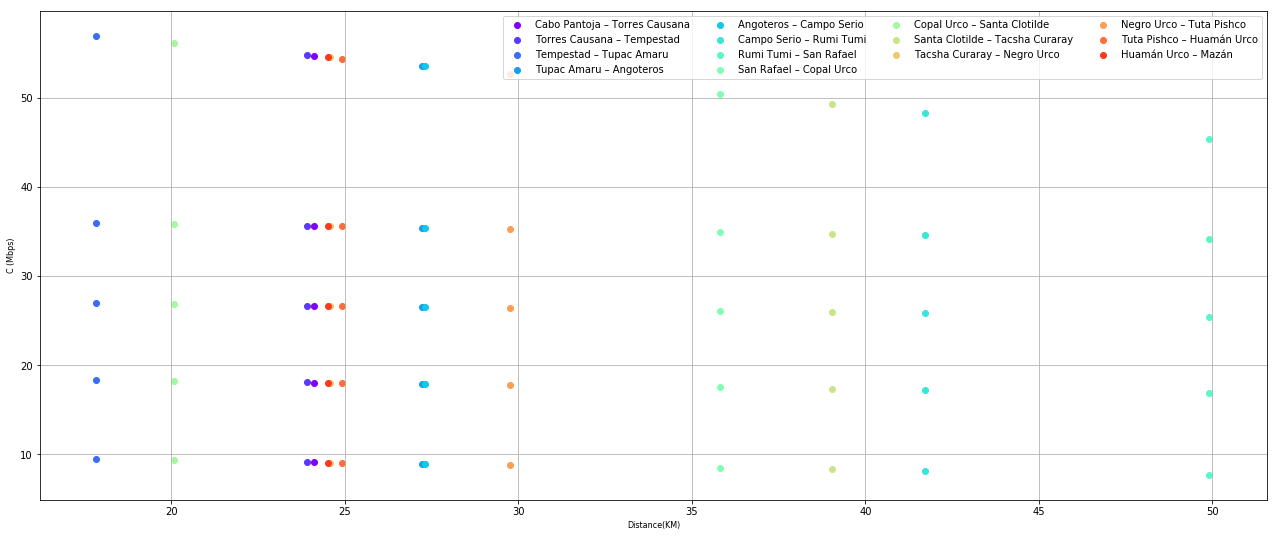
\includegraphics[width=0.7\textwidth]{img/valoresmbps.png}
		\caption{Capacidad del canal teórica respecto a la distancia para cada MCS con NV2}
		\label{valoresmbps}
	\end{figure}
	
	Los valores obtenidos y representados corresponden a las modulaciones comprendidas entre MCS8 y MCS12, no obstante el interés de este estudio es determinar cúal sería la modulación mínima utilizable de forma teórica en la red del Napo, asegurando así esa capacidad mínima definida de 44 Mbps por radioenlace. Cómo se ha comentado al inicio del capítulo se realizó una estimación para el ancho de banda correspondiente al proyecto, doblando los valores de \textit{throughput} existentes en las coordenadas base.\\\\
	
	En conclusión a este análisis teórico y aproximación analítica, la tabla \ref{table:capacidades} recoge los datos obtenidos, los cuáles reflejan que para cumplir con los requesitos necesarios de la red cada radioenlace debe utilizar una modulación MCS10.   
	
\subsection{Estudio con RadioMobile}
	Una vez desarrolado el estudio teórico sobre la red, nuestro siguiente paso será realizar una representación simulada con el objetivo de obtener más información sobre la viabilidad de enlace relativa a los emplazamientos del proyecto. Para ello, utilizaremos los datos de geolocalización y distancia relacionados con los emplazamientos de la red del Napo los cuáles se encuentran en las tablas \ref{table:distancias} y \ref{table:geolocalizacion}, para introducirlos en la herramienta RadioMobile y crear así nuestra red simulada. Junto a la localización geográfica y altura de cada emplazamiento tendremos que configurar los principales parámetros de la red y de los equipos en la herramienta, esta combinación nos permitirá obtener una aproximación sobre la calidad del enlace en términos generales e individuales de la red. A continuación se detallan las características de los sistemas insertados en la herramienta para llevar a cabo la simulación:
	\begin{itemize}
		\item Potencia de transmisión: 32 dBm
		\item Sensibilidad en recepción: -96 dBm
		\item Pérdidas por cable: 1,5 dB
		\item Ganancia de antena: 30 dBm
		\item Tipo de antena: Omnidireccional
		\item Frecuencia: 5260 MHzs
	\end{itemize}
	Una vez configurado los parámetros y características de los sistemas, obtenemos una representación simulada de la red tal y como se muestra en la figura \ref{redNapo}. Dicha simulación está sujeta al modelo \textit{Longley-Rice} que utiliza la variabilidad de tiempo, posición y situación para realizar los cálculos respecto al balance de enlace.  
	\begin{figure}[H]
		\centering
		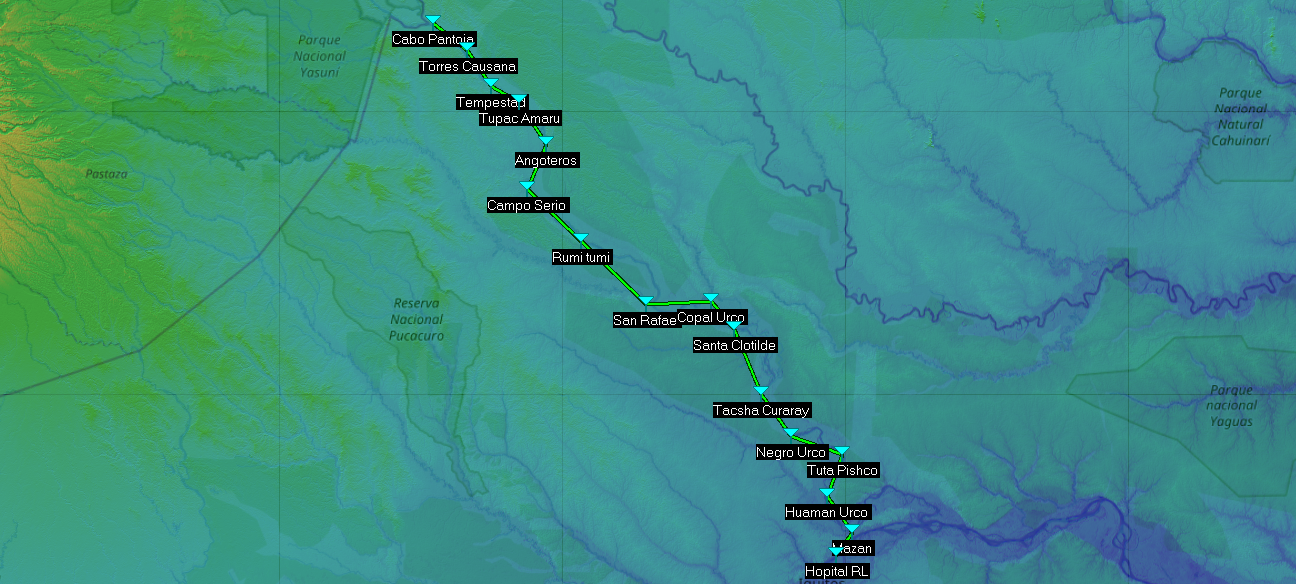
\includegraphics[width=0.7\textwidth]{img/redNapo.PNG}
		\caption{Representación de la red del Napo en RadioMobile}
		\label{redNapo}
	\end{figure}
	La funcionalidad \textit{Radio Link} que se encuentra dentro de RadioMobile, nos permite obtener una representación simulada del estado de cada radioenlace a través de la recreación del perfil geográfico y configuración de los sistemas involucrados en el enlace. Esto nos permite conocer los niveles de pérdidas, sensibilidad en recepción y margen dinámico de cada sistema de forma individual a través de la realización del balance de enlace. Dicho balance de enlace nos proporcionará información respecto a la sensibilidad y potencia en transmisión y recepción, para poder establecer la mínima tasa de transmisión soportada siempre y cuando, cumpla con los requisitos de viabilidad de enlace mencionados al principio de este Trabajo Fin de Grado.\\\\
	
	Para poder obtener una tasa mínima que cumpla los requisitos de transmisión mínimos mencionados en el capítulo de introducción, debemos tener en cuenta el tipo de tecnología que estamos utilizando. En nuestro caso, las transmisiones pertenencientes a la nueva red del Napo se realizarán utilizando la tecnología \textit{Multiple Input Multiple Output}, junto al uso de NV2 como protocolo de acceso al medio. La utilización de MIMO hace que nos centremos en los valores pertenecientes a las MCS cuyos valos están comprendidos entre MCS8 y MCS15, dichas MCS a su vez están formadas desde una constelación BPSK (formada por dos símbolos) hasta una 64-QAM (formada por 64 símbolos). Para poder establecer una comparación entre la modulación adecuada por cada radioenlace tendremos que comparar la senbilidad en recepción de cada sistema obtenido mediante la simulación, con los valores típicos de sensibilidad para dichas MCS.\\\\
	
	Los valores obtenidos a través de la simulación por cada radioenlace y los valores respecto al protocolo NV2 en términos de sensibilidad han sido recogidos en las siguientes tablas:\\\\
	
	En conclusión habiendo estudiado las diferentes situaciones y analizado las características de los radioenlaces cuyos resultados se recopilan en la siguiente tabla. En función de los valores obtenidos en la simulación y, teniendo en cuenta los resultados conseguidos mediante el estudio teórico previo, podemos destacar lo siguiente: 
	\begin{itemize}
		\item Existe línea de visión directa en la mayoría de casos, lo que implica asegurar la zona de Fresnel mínima para la viabilidad del enlace, en nuestro caso un sesenta por ciento.
		\item Habiendo analizado cada balance de enlace de forma individual podemos realizar una extrapolación para el total de la red, asegurando así un margen dinámico que garantice la viabilidad del enlace. En el caso del diseño inicial dicho margen dinámico era de 20 dB, por tanto habiendo contrastado los datos obtenidos con la simulación no existe compromiso respecto a la viabilidad de enlace en cada punto de la red.
		\item En base al estudio análitico hecho, para asegurar la total funcionalidad de la red, habría que utilizar un MCS10 como mínima para alcanzar una capacidad de enlace suficiente y necesaria.
	\end{itemize}
	
\subsection{Configuración de equipos}
Para poder recrear en laboratorio un escenario punto a punto de similares características a los de la red del Napo, utilizaremos dos equipos NetMetal 5 y dos portátiles con distribuciones Linux. Los ordenadores portátiles actuarán de emisor y receptor en nuestra red local junto a los equipos NetMetal 5 que interconectarán dichos terminales finales entre sí, como se muestra en la figura \ref{enlace}. Para obtener valores relacionados con los parámetros de QoS se inyectará tráfico con la herramienta Iperf y Bandwidth test, utilizando uno de los portátiles como cliente y otro como servidor.\\\\

\begin{figure}[H]
	\centering
	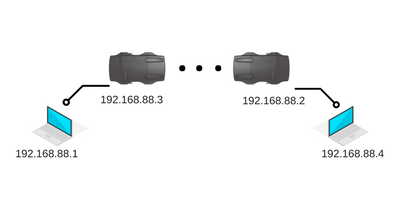
\includegraphics[width=0.7\textwidth]{img/escenario.png}
	\caption{Escenario de laboratorio punto a punto}
	\label{enlace}
\end{figure}

Antes de comenzar a detallar como se ha realizado la configuración a nivel de laboratorio de los equipos, debemos apuntar qué, en nuestro caso las antenas utilizadas son dipolos elementales colocados en posición vertical y horizontal transmitiendo forma multimodal, en el caso del proyecto Napo cada radioenlace constará de una antena parabólica colocada en lo alto de una infraestructura metálica, cuya ganancia de transmisión está en torno a los 30 dB. \\\\

\section{Inyección de tráfico simulado}
Para conocer el rendimiento y prestaciones de los equipos realizaremos pruebas a nivel de red a través de la inyección de tráfico simulado. Para llevar a cabo dicha prueba, utilizaremos el software disponible para los sistemas operativos de distribución Linux Iperf y la herramienta de medida de ancho de banda proporcionada por MikroTik Bandwidth text, las cuáles se detallan brevemente a continuación.\\\\

\subsection{Iperf}
Iperf \cite{Iperf} es una herramienta que permite realizar mediciones sobre el máximo rendimiento alcanzable respecto al ancho de banda y la calidad de un enlace red. Esto es posible mediante el análisis y recopilación de datos referentes a los protocolo de red TCP y UDP. Existe la variante Jperf, cuya única diferencia es la utilización de una interfaz gráfica en lugar de la entrada estándar de comandos.\\\\

La herramienta puede ser utilizada en modo cliente o en modo servidor, permitiendo realizar pruebas sobre la red hasta obtener los valores óptimos sobre la misma, tal y como se muestra en la figura \ref{logTestIperf}.\\
Esto es gracias al ajuste y modificación de parámetros que permite la herramienta: según sea nuestro escenario y el objetivo de nuestras pruebas, podremos obtener un tipo específico de datos u otros. La elección de los parámetros de la herramienta será diferente según el protocolo de red (TCP o UDP) que utilicemos en cada caso. A continuación detallamos las posibilidades que ofrece en base a cada uno de ellos:\\\\

En primer lugar explicaremos los parámetros relacionados al protocolo UDP, el cual nos permite seleccionar un ancho de bando específico en nuestra comunicación y permite utilizar multidifusión si fuera necesario. Además, los datos reportados por la herramienta en este caso son los relacionados con la pérdida de paquetes, ya sea en cuantía o en porcentaje, y las medidas relacionadas con el jitter y retardo.\\
En segundo lugar, los parámetros configurables respecto a TCP están relacionados con la elección de un tamaño de ventana TCP fijo para la comunicación, otorgando datos respecto al ancho de banda medido en la comunicación y el tamaño MSS/MTU.

\begin{figure}[H]
	\centering
	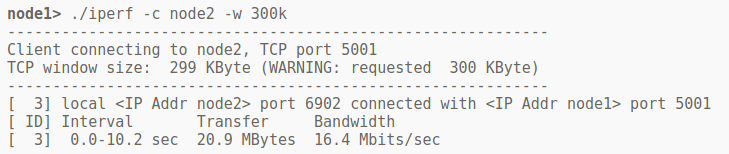
\includegraphics[width=0.7\textwidth]{img/log_iperf.png}
	\caption{Log obtenido al realizar una prueba con Iperf}
	\label{logTestIperf}
\end{figure}

\subsection{Bandwidth test}
\textit{Bandwidth test} es la herramienta desarrollada por el fabricante que nos permite realizar medidas entre equipos MikroTik en lo que a \textit{throughput} se refiere. Dicha herramienta está disponible tanto para la interfaz web, cómo para la consola.\\\\

Para llevar a cabo dicho test, debemos configurar uno de los routers que forman la red en modo servidor, y el resto en modo cliente, además la herramienta nos proporciona una serie de parámeotros configurables respecto a la red activa tales cómo: dirección, duración, tamaño de paquete, etc... \\
En función de estos parámetros el resultado de la prueba será de un modo u otro, y nos proporcionará los valores deseados respecto a el número de paquetes pérdidos, velocidades medias y totales en recepción y transmisión de la conexión activa. A continuación, en la figura \ref{logTest} se muestra un ejemplo del log obtenido al realizar una prueba utilizando la herramienta mencionada anteriormente.

\begin{figure}[H]
	\centering
	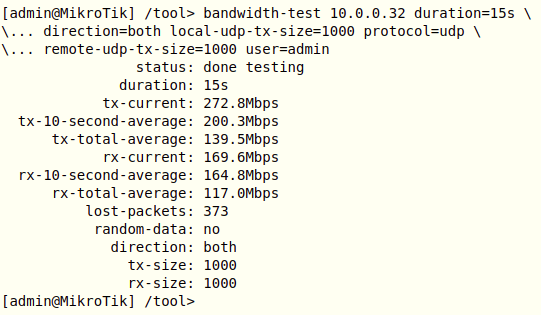
\includegraphics[width=0.7\textwidth]{img/log_test.png}
	\caption{Log obtenido al realizar una prueba sobre un enlace MikroTik activo}
	\label{logTest}
\end{figure}

\subsection{Configuración y realización de pruebas}

\section{Monitorización y gestión: Zabbix}
En esta sección se explicará la integración llevada a cabo con el escenario configurado en laboratorio y el \textit{software} de monitorización Zabbix. Así mismo, se procederá a explicar de manera más detallada el funcionamiento de la herramienta seleccionada en el marco contextual definido al inicio de este Trabajo Fin de Grado.\\\\

Antes de realizar la configuración del escenario formado en laboratorio, se procede a explicar cómo se va a llevar a cabo la integración de Zabbix y dicho escenario. Esto se llevará a cabo mediante el uso de plantillas XML y el protocolo SNMP el cúal, nos permite intercambiar información entre los dispositivos involucrados.\\
 
El protocolo SNMP (\textit{Simple Network Management Protocol}) es un protocolo que corresponde con la capa de aplicación y facilita el intercambio de información administrativa entre los dispositivos que componen una red, ya sean \textit{routers}, \textit{switches}, etc... Este protocolo facilita a los administradores de red conocer en todo momento el estado de la red, así cómo la posibilidad de interactuar con la misma tomando acciones de prevención, resolución de problemas y estudio sobre escalabilidad.\\
Para lograr esto, SNMP accede a la MIB (\textit{Management Information Base}) de los equipos. La MIB es una colección de información referente al equipo organizada de forma jerárquica mediante un árbol, para llevar a cabo una eficiente búsqueda y consulta de los objetos que se encuentran dentro del árbol, se organizan en subconjuntos denominados organizaciones.\\\\

Cada objeto, denominado OID (\textit{Object Identifier}) contiene un valor asociado al parámetro que representa, ya sea en formato de cadena de carácteres o en formato numérico, para conseguir dicho valor se ha de realizar una búsqueda descendente del árbol que forma la MIB, ya sea bien utilizando la nomenclatura numérica que tiene cada organización seguida de un punto (1.3.6....) o bien utilizando el nombre de cada organización seguido de un punto (iso.identified....). Ambos métodos permiten recuperar el valor del parámetro deseado y utilizarlo en nuestra integración.\\\\

Así mismo, el funcionamiento de SNMP involucra a los siguiente agentes:

\begin{itemize}
	\item Sistema administrador: Capaz de ejecutar aplicaciones (comandos) capaces de controlar los dispositivos involucrados en la red, proporcionando métricas útiles para el administrador en cuánto a los recursos del equipo.
	\item Dispositivo administrado: Equipo que contiene el agente SNMP y forma parte de la red recogiendo información usando el protocolo SNMP.
	\item Agente SNMP: Permite realizar una administración de la forma otorgada por el equipo de manera local y jerarquizarlo en forma de árbol y en un formato compatible al intercambio de información usando dicho protocolo.
\end{itemize}

SNMP no sólo nos permite recorrer el árbol MIB y obtener información de los equipos, sino que mediante aplicaciones (comandos), es posible realizar simples operaciones sobre la estructura jerarquizada de los equipos, dichos comando se describen a continuación:

\begin{itemize}
	\item Lectura/Escritura: Permiten al administrador leer/modificar los valores de las variables almacenados dentro de los dispositivos.
	\item Notificación: Permite a los equipos reportar eventos de manera asíncrona al administrador. 
	\item Transversales: Permiten a los equipos recolectar información de los elementos cercanos en la red y conformar tablas relacionadas a la información obtenida. 
\end{itemize}

\subsection{Integración de escenario}
Una vez explicado todo lo que implica el uso de SNMP y la jerarquización de los objetos existente en los equipos y cómo es posible realizar consultas a dichos objetos, procedemos a explicar cómo se va a integrar la información procedente de los equipos con Zabbix. Una de las facilidades que nos ofrece la herramienta es que podemos crear \textit{items} tal y como se muestra en la figura \ref{xmlTest}, aprovechando la información que nos proporcionan los OIDs en función de los parámetros que deseemos monitorizar. Para ello deberemos seguir el estándar XML, utilizando una plantilla como la mencionada antes e importarla en el sistema. De igual forma, que podemos importar datos existe la posibilidad de exportarlos, ofreciendo así versatilidad a la hora de integrar cualquier equipo en un sistema diferente. En el marco del proyecto los principales parámetros de interés son los referentes a salud de los equipos (carga CPU, temperatura, etc...) y a tráfico obtenido. 

\begin{figure}[H]
	\centering
	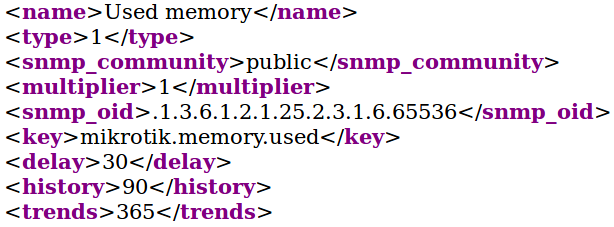
\includegraphics[width=0.7\textwidth]{img/xml_example.png}
	\caption{Ejemplo de configuración de un item sobre XML en Zabbix}
	\label{xmlTest}
\end{figure}

Una vez cargados los dispositivos involucrados en la plataforma, Zabbix ofrece varias herramientas para realizar un seguimiento sobre dichos elementos y otorgar control total sobre ellos al administrador, como por ejemplo configurando \textit{dashboards} de seguimiento, alertas sobre equipos, creación de mapas de redes, etc... A continuación se procede a detallar algunas de las aplicaciones utilizadas en este Trabajo Fin de Grado cuyo objetivo es monitorizar y obtener un control total de la red:\\\\

En primer lugar, nos hemos centrado en la representación gráfica del rendimiento que otorgan los equipos a nivel de red, para ello, hemos utilizado la aplicación que ofrece la propia herramienta que permite realizar gráficas a nivel de interfaz, como se muestra en la figura \ref{zabbixMeasure}, una aplicación interesante de estas gráficas es que se puede realizar un tablero configurable conjunto, es decir, integrar dicha gráfica (o similares) de diferentes dispositivos en un único tablero, otorgando así al administrador una visión global del tráfico entrante y saliente de la red en conjunto.

\begin{figure}[H]
	\centering
	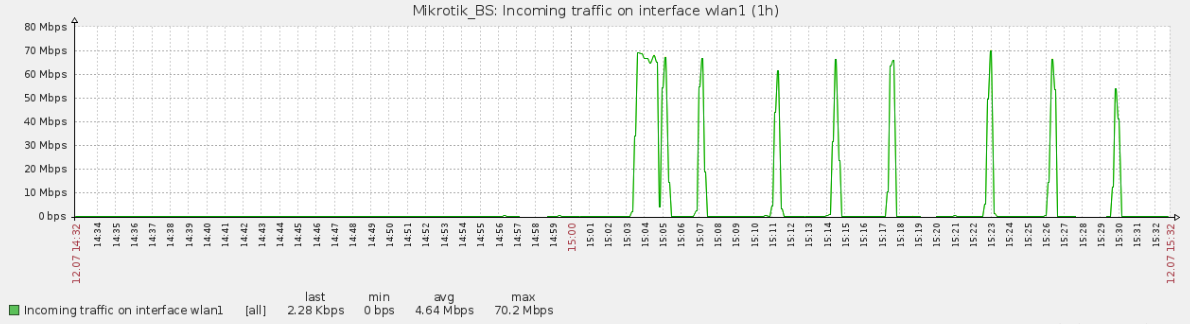
\includegraphics[width=0.7\textwidth]{img/zabbix_measure.png}
	\caption{Ejemplo de representación gráfica de tráfico mostrado en un Dashboard de Zabbix}
	\label{zabbixMeasure}
\end{figure}

En segundo lugar, Zabbix ofrece alertas configurables en función de los \textit{items} cargados en la plantilla XML tal y como se muetra en la figura , esto quiere decir que la herramienta ofrece \textit{triggers} configurables, ya sea bien de forma predeterminada o personalizada, que permiten establecer valores umbral para los diferentes niveles de alerta que ofrece la herramienta, generando así una categorización de problemas y otorgando al administrador una versión prioritaria de la acción que ha de ser tomada. Las alertas no son configuradas únicamente si el programa se está ejecutando en primer plano, Zabbix ofrece una extensión llamada PostFix \cite{PostFix} que permite integrar y configurar alertas para que sean enviadas mediante email.\\
De igual forma, Zabbix mantiene un archivo histórico de logs el cúal otorga cierta ventaja a la hora de actuar al administrador, ya sea en labores de mantemiento de la red o bien en labores predictivas. 

\begin{figure}[H]
	\centering
	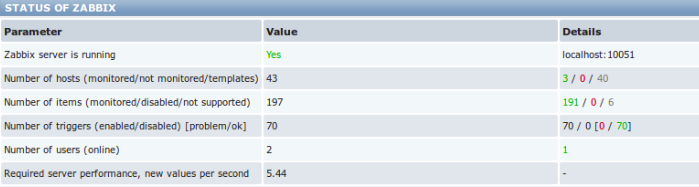
\includegraphics[width=0.7\textwidth]{img/zabbix_resume.png}
	\caption{Ejemplo del estado de la red en Zabbix}
	\label{zabbixResume}
\end{figure}

Por último, otra aplicación interesante en el marco del proyecto es la creación de mapas de red, como muestra la figura \ref{zabbixNetwork}, la cúal permite al administrador no sólo jerarquizar los equipos en función de nombres o por IPs, si no que otorga la posibilidad de subdividir una red total en subredes de forma que puedan aislarse cada una de ellas en subconjuntos, consiguiendo así un análisis más rápido y eficaz que si tuviera que realizarse de toda la red en conjunto. Aparte de esto, subdividir las redes porporciona la capacidad de asignar cada subred a un grupo de técnicos determinado evitando así que la gestión de una única subred involucre al resto de la misma.

\begin{figure}[H]
	\centering
	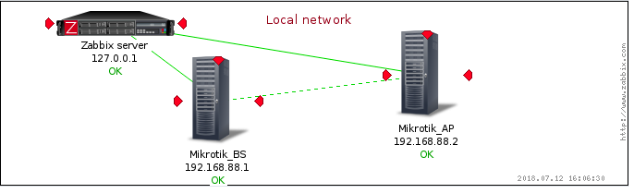
\includegraphics[width=0.7\textwidth]{img/zabbix_networks.png}
	\caption{Ejemplo de jerarquización de redes en Zabbix}
	\label{zabbixNetwork}
\end{figure}

En definitiva y reuniendo todo lo explicado a lo largo de este capítulo, Zabbix no sólo es una solución que cumple con los requisitos mínimos de monitorización de redes requeridos en el proyecto, si no que su amplia variedad de integraciones y aplicaciones.Zabbix no sólo permite una fácil integración con los dispositivos físicos mediante el uso de plantilla XML y protocolo SNMP, si no que también ofrece una solución a todo lo referido con \textit{software} de terceros. Todo esto a partir de la editabilidad de la mayor parte su funcionalidad básica para hacer que el administrador de redes tenga la mayor cantidad de información sobre los equipos, concentrada de tal forma que su actuación se inminente y precisa si esta fuera requerida.
	\chapter{Selección de equipamiento, despliegue y diseño de la red}
\label{cap:equipamiento}

\section{Comparación entre equipos}	
Antes de proceder a comparar los equipos introducidos anteriormente, debemos primero explicar el protocolo de pruebas que se ha elaborado con la colaboración de los compañeros involucrados pertenecientes a la PUCP. Dicho protocolo nos servirá para valorar y evaluar las prestaciones de cada uno de los equipos de forma individual y establecer una comparativa, con el fin de obtener una solución lo más viable y factible posible en lo que al marco del proyecto se refiere. \\

 Primeramente se van a establecer, con ayuda de RadioMobile, los requisitos mínimos de los equipos que pueden ser elegibles para su uso en los enlaces de la red que se va a desplegar; a partir de esos requisitos, se ha diseñado un protocolo de pruebas en colaboración con la PUCP que comporta revisión de las especificaciones y pruebas de campo con los equipos. Las pruebas de campo conllevarán la configuración de un enlace punto a punto en las instalaciones disponibles para dicho efecto de la PUCP. Una vez configurado el enlace, se realizarán pruebas de conectividad utilizando programas para inyectar tráfico y se examinarán los valores obtenidos. De forma simultánea, se registrarán los valores energéticos proporcionados por los equipos durante las pruebas para valorar su eficiencia energética.\\
 
 Las pruebas realizadas por la PUCP han sido llevadas a cabo en diferentes emplazamientos, ubicados en Iquitos-Mazán para el caso de los equipos Net Metal 5 y RM-MAX, y por otro lado para los equipos Ubiquiti en los emplazamientos encontrados en Pachatutec (Ventanilla) y San Miguel. Aunque a simple vista parezca que la ubicación de los emplazamientos seleccionados es muy dispar, la infraestructura existente y sus perfiles geográficos son muy parejos, por lo tanto nos sirve como escenario para realizar nuestro análisis. De igual forma, este estudio se ha tenido que realizar de forma interrumpida, es decir primero una pareja de equipos y después la otra, debido a las disponibilidad de los emplazamientos y equipos.\\
 
 La configuración de ambos escenarios sigue un esquema similar al mostrado en la Figura \ref{pruebasPUCP}, en este caso particular se hace referencia al enlace existente entre Mázan y el hospital regional de Loreto y las características utilizadas para el desarrollo de pruebas en dicho emplazamiento. No obstante esta arquitectura es la utilizada a lo largo de todos los emplazamientos que conforman la red del Napo, dicha arquitectura está compuesta por torres metálicas y equipos portátiles en los cuales se realizarán las mediciones de tráfico y se medirá el rendimiento de los equipos.
 
 \begin{figure}[H]
			\centering
			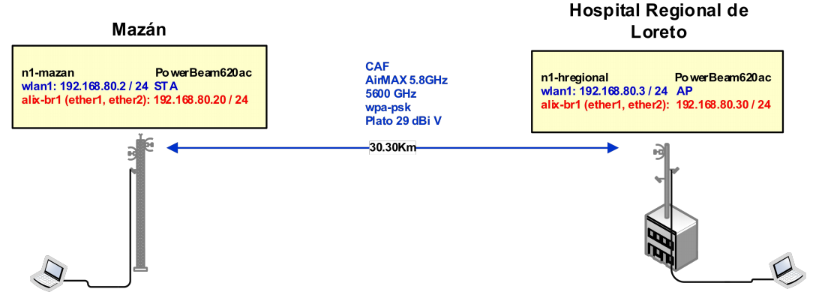
\includegraphics[width=0.7\textwidth]{img/enlace.PNG}
			\caption{Escenario de pruebas propuesto por PUCP.}
			\label{pruebasPUCP}
\end{figure}

Antes de comenzar a detallar los resultados obtenidos en cada una de las pruebas realizadas, debemos aclarar los criterios y exigencias mínimas a las que los equipos han sido sometidas. Dichos requerimientos se describen a continuación:

\begin{itemize}
    \item La gestionabilidad de los equipos se realizará mediante el protocolo SNMP, por tanto debemos disponer de la MIB del fabricante y programa para gestionar los equipos con el objetivo de monitorizar y configurar las pruebas a realizar.
    \item Diseñar un perfil virtual obtenido a través de RadioMobile configurado con las características de los equipos.
    \item La calidad del radio enlace establecido ha de tener un nivel de señal satisfactorio. Considerando satisfactorio una potencia de señal recibida que quede al menos 15 dB por encima de la sensibilidad del modo de transmisión más robusto que sea utilizable.
\end{itemize}

Por último, y en adición a todo lo comentado anteriormente, se crearán unos cuadros de emparejamiento con los equipos y sus principales características junto a los datos obtenidos en las pruebas para así extraer una conclusión sobre qué equipo es el propuesto como solución en este proyecto.

\subsection{Comparación NetMetal 5 - RM-MAX}
 Este primer análisis se ha llevado a cabo en los emplazamientos de San Miguel y Ventanilla los cuales están separados por una distancia de 29 Km y disponen de torres con antenas cuya ganancia es de 34 dBi en la banda de 5 GHz. Para llevar a cabo las pruebas de tráfico  y eficiencia se han tenido en cuenta los resultado obtenidos en los perfiles obtenidos con la simulación, correspondientes a las imágenes \ref{mikro_sanmiguel} y \ref{mikro_rmmax}; y los datos recopilados en la Tabla \ref{table:parámetrosEquipos} que identifican los principales parámetros de los equipos.\\
 
  \begin{figure}[H]
			\centering
			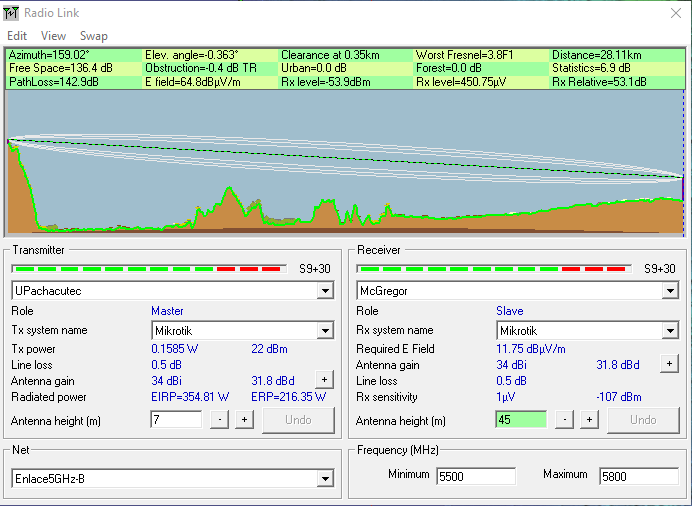
\includegraphics[width=0.6\textwidth]{img/Mikrotik_pruebas.png}
			\caption{Simulación realizada con la configuración de equipos NetMetal 5 entre las estaciones de San Miguel y Ventanilla}
			\label{mikro_sanmiguel}
\end{figure}
 \begin{figure}[H]
			\centering
			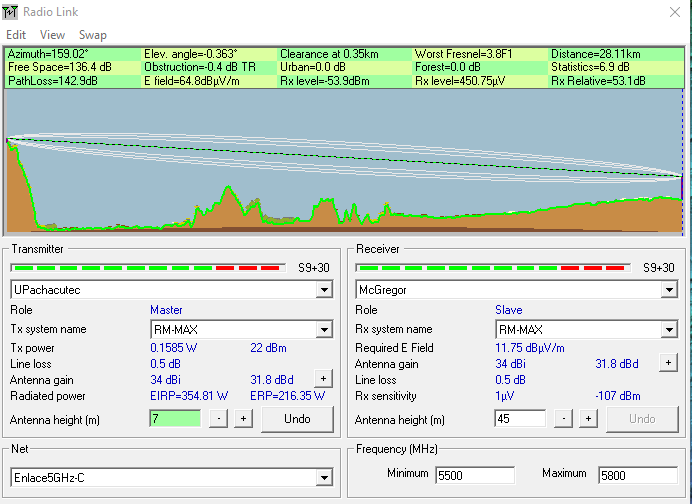
\includegraphics[width=0.6\textwidth]{img/rmmax_pruebas.png}
			\caption{Simulación realizada con la configuración de equipos RM-MAX entre las estaciones de San Miguel y Ventanilla}
			\label{mikro_rmmax}
\end{figure}
 Una vez identificado los primeros valores de viabilidad del enlace, el siguiente paso es realizar pruebas teniendo en cuenta la variación de ancho del canal y la modulación utilizada. En este caso se utilizó la frecuencia de 5745 MHz como frecuencia operacional, y 20 - 40 MHz como valores de ancho de banda. Por último, se determinó fijar el valor de la modulación de transmisión en una MCS11, correspondiente a una constelación 16QAM, por considerarse la más robusta elegible en función de la capacidad binaria que va a brindar. Los resultados obtenidos se muestran en la Tabla \ref{table:pruebasEquipos}; dicha tabla recoge los promedios obtenidos en cuanto al porcentaje de paquetes pérdidos, retardo y \textit{throughput}.\\ 
Una vez examinado los datos obtenidos en las pruebas realizadas vemos como los equipos Mikrotik ofrecen mejor rendimiento y prestaciones tanto para el ancho de canal de 20 MHz como para el de 40 MHz respecto al equipo RM-MAX. \\

Mientras que los equipos RM-MAX tienen un \textit{throughput} de 1,42 Mbps, 46\% de paquetes pérdidos y 223 ms de retardo todo ello para 20 MHz, frente a los 10 Mbps, 12\% y 11 ms que ofrecen los equipos Net Metal 5. Para el ancho de banda de 40 MHz los resultados siguen siendo iguales, para los valores de 45 Kbps, 63\% y 168 ms que ofrecidos por los equipos RM-MAX, los equipos NetMetal 5 ofrecen valores de 24,32 Mbps, 0,46\% y 10 ms.\\

En cuanto al consumo energético, los equipos NetMetal 5 consumen 8,35 W mientras que los equipos RM-MAX llevan su consumo hasta 14,29 W de potencia.\\

A la vista de los resultados, los equipos NetMetal 5 son los equipos elegidos como solución frente a los RM-MAX. 

\subsection{Comparación PowerBeam AC - AirFiber }
Para este segundo análisis los emplazamientos escogidos fueron los ubicados en Mazán e Iquitos entre los cuales existe una distancia de aproximadamente 31 Km. Para llevar a cabo estas pruebas y perfiles greográficos con RadioMobile, se parametrizaron las configuraciones de los equipos acorde a la Tabla \ref{table:parámetrosEquiposUbiquiti} y teniendo en cuenta las restricciones existentes en cuanto a la potencia isotrópica radiada equivalente (PIRE), la cual se establece en 49 dBm para el primer rango de frecuencias y en 54 dBm para el cuarto rango de frecuencias.\\

Por un lado, para conocer la viabilidad del enlace y establecer un mínimo de potencia que garantice la estabilidad del mismo, se han utilizado los perfiles obtenidos en la simulación, dichos perfiles están ubicados a contiuación en la Figura \ref{simulacionUbiquiti}. Una vez analizado los perfiles se observa como para el primer rango de frecuencias, existe un limitación de potencia transmitida a nivel legislativo, por tanto nuestra simulación no puede exceder dichos valores. El resultado de la simulación establece que el mínimo de potencia de señal recibidad es de 21,9 dBm con los equipos AirFiber y 23,2 dBm para los equipos PowerBeam.

\begin{figure}[H]
\centering
\subfigure[Simulación con PowerBeam AC]{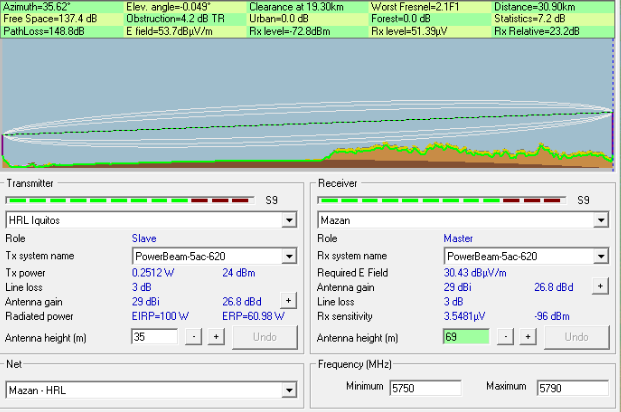
\includegraphics[width=70mm]{img/PowerBeamAC.PNG}}\hspace{2mm}
\subfigure[Simulación con AirFiber con 24 dBm de potencia de transmisión ]{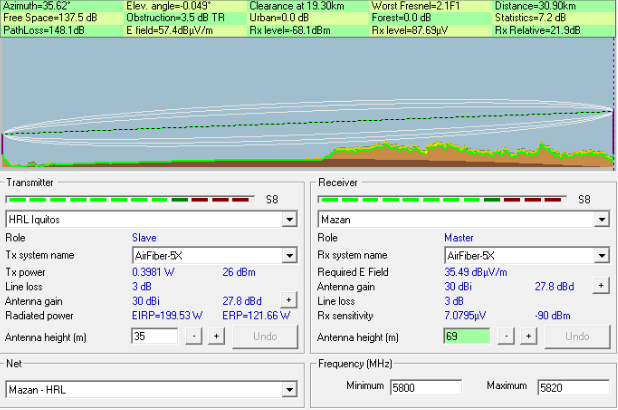
\includegraphics[width=70mm]{img/AirFiber5x.PNG}}\vspace{2mm}
\subfigure[Simulación con AirFiber con 22 dBm de potencia de transmisión]{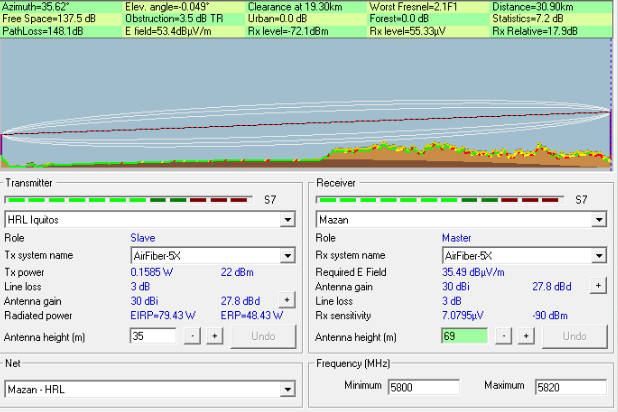
\includegraphics[width=70mm]{img/AirFiber5x_22dBm.PNG}}\hspace{2mm}
\subfigure[Simulación con AirFiber con 9 dBm de potencia de transmisión]{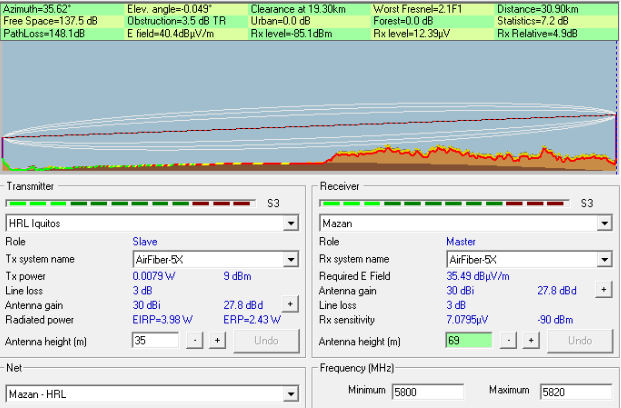
\includegraphics[width=71mm]{img/AirFiber5x_9dBm.PNG}}\vspace{2mm}
\caption{Simulación de los equipos Ubiquiti en el escenario Mazán-Iquitos} \label{simulacionUbiquiti}
\end{figure}

A parte de las pruebas con el escenario  simulado, se llevaron a cabo pruebas a nivel de campo con los equipos con el objetivo de conocer el rendimiento de cada uno de ellos; dichos resultados se adjuntan en la Tabla \ref{table:pruebasEquiposUbiquiti}. Una vez recopilados todos los datos y analizados, se extraen las siguientes conclusiones:

\begin{itemize}
    \item Bajo las condiciones de este escenario, los equipos PowerBeam son más estables utilizando un canal de 20 MHz, obteniendo una tasa de transferencia promedio de 40 Mbps. Por otra parte,los equipos AirFiber están alcanzando promedios de 37 Mbps utilizando un canal de 40 MHz y 78 Mbps utilizando un canal 50 MHz, aunque en ambos casos el enlace presenta inestabilidad.
    \item El retardo ofrecido por los equipos AirFiber es mucho mejor que el de los equipos PowerBeam.
    \item En la estación de Iquitos existe una abundante interferencia electromagnética lo que implica configurar de forma fija la modulación máxima, en Mazán se alcanza la modulación 64QAM mientras que en Iquitos se llega a la modulación 16QAM. En las mejores condiciones usando Powerbeam con un ancho de canal 20 MHz y retardos considerables conseguimos transmitir con la modulación de 64QAM; sin embargo, en el caso de Airfiber se consigue transmitir con una modulación de 16QAM con un ancho de canal de 40 MHz y bajo retardo.
\end{itemize}

Una vez comtemplando los diferentes equipos y habiendo realizado pruebas en el escenario destinado para ello y en entornos simulados, los equipos propuestos como solución a usar en el marco de este proyecto son los NetMetal 5. Gracias a su mejor rendimiento en el conjunto global de la evaluación, teniendo en cuenta su eficiencia energética, versatilidad a la hora de establecer configuraciones y manejo de la herramienta de configuración, desempeño durante las pruebas de ancho de badna y tráfico.

\section{Configuración y diseño de la red}
Antes de realizar el montaje del escenario y realización de pruebas en laboratorio, debemos realizar un diseño y estudio sobre la red. Dicho análisis nos permitirá conocer de forma más detallada los diferentes factores que pueden comprometer la viabilidad de los diferentes enlaces que componen la red, y así ajustar la configuración de los equipos a dichos factores para garantizar el objetivo y requisitos predefinidos en el proyecto.\\

Tras la conlcusión de la parte correspondiente al estudio y diseño de la red, realizaremos nuestras simulaciones a nivel de laboratorio. El objetivo de esto será establecer una comparación con los resultados obtenidos en la fase de estudio; para ello dispondremos de los equipos NetMetal 5 y ordenadores con sistema operativo GNU/Linux, ya que este sistema operativo da facilidades añadidas a la hora de instalar y manejar los programas necesarios para la realización de pruebas. Las pruebas llevadas a cabo determinarán el rendimiento que ofrecen los equipos NetMetal 5 en lo que a conectividad y parámetros de calidad se refiere.

\subsection{Estudio previo} 
	En esta sección procederemos a realizar un estudio teórico cuantitativo del \textit{throughput} que se puede esperar en cada uno de los radioenlaces que forman la red del Napo. Para ello utilizaremos los valores empíricos obtenidos en el artículo \cite{simo2014assessing} recogidos en la Tabla \ref{table:pruebasNV2campo}, obtenidos a través de la realización de pruebas de campo con el protocolo NV2 y un ancho de banda de 20 MHz.\\
	
	Por una parte, los valores presentes en dicha tabla corresponden a medidas de capacidad en radioenlace para una distancia de 0 Km (medidas en laboratorio) y una distancia de 30 Km, las medidas fueron llevadas a cabo desde la modulación MCS0 hasta MCS15 para la mayoría de casos, salvo en las mediciones de 30 Km, qué para valores superiores a MCS11 no se pudieron realizar pruebas empirícas. No obstante, sólo nos apoyaremos y tomaremos como referencia los valores comprendidos entre la modulación MCS8 y MCS11 ya que son las modulaciones destinadas para el uso de MIMO. \\
	Por otra parte, dichas medidas corresponden a la utilización de 20 Mhz como ancho de banda, para poder establecer una relación con el ancho de banda utilizado en el proyecto se procederá a duplicar los valores obtenidos a 20 Mhz. Obteniendo así un aproximación de los valores teóricos que deberían ser obtenidos de forma empiríca para un ancho de banda de 40 Mhz; una vez concluida la parte teórica se contrastarán dichos valores con los obtenidos en laboratorio y se procederá a realizar un análisis más exhaustivo.\\
	
	Para poder llevar a cabo el estudio teórico, se han recogido los valores antes mencionados y se han organizado en pares de coordenadas obteniendo un conjunto de datos que establecen una relación entre: la distancia, el \textit{throughput}, y el valor de la modulación MCS utilizado. Una vez acondicionados los datos, se ha proyectado una recta lineal entre los puntos pertenecientes a cada MCS respecto a las coordenadas base de 0 Km y 30 Km, con el objetivo de obtener una recta que pase por todos los puntos de interés de nuestra red, tal y como muestra la Figura \ref{rectaspendiente}, permitiendo establecer así una aproximación teórica de la capacidad del enlace en función de la distancia.\\
	
	De forma paralela, en base a la obtención de las rectas respecto a cada MCS hemos podido realizar una estimación de la capacidad teórica que debería de existir para cada radioenlace; dicha estimación se muestra en la Figura \ref{valoresmbps}. Para llevar a cabo todo el estudio teórico y todo el desarrollo comentado anteriormente, se ha utilizado el script \ref{lst:script}, que está desarrollado en el lenguaje de programación Python, ya que permite la integración de módulos y librerías de análisis matemático de forma sencilla.
	
	\begin{figure}[H]
		\centering
		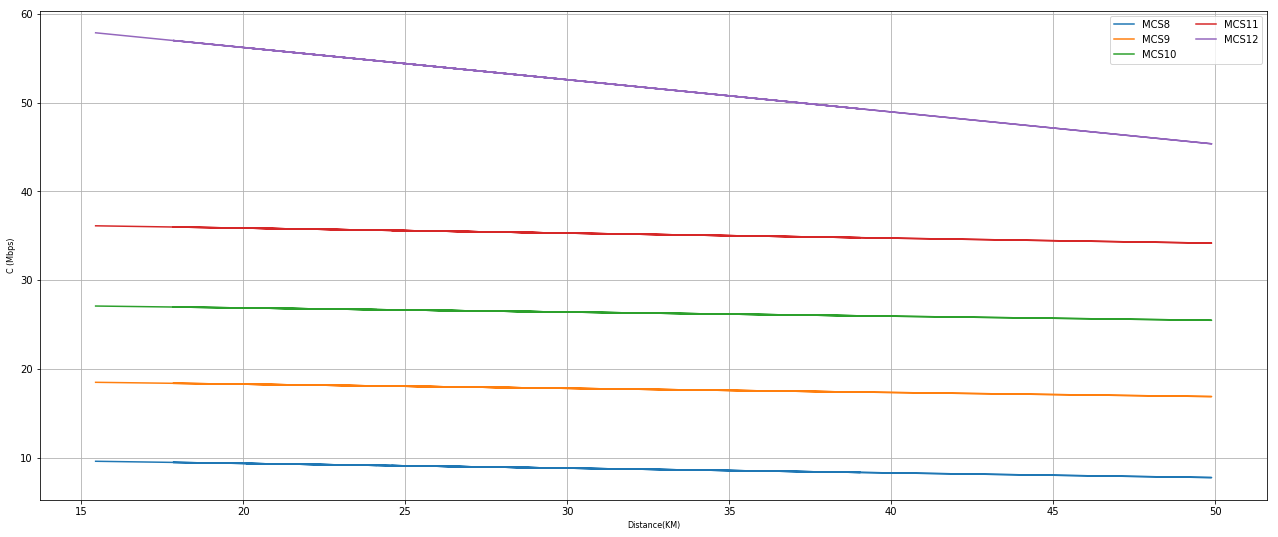
\includegraphics[width=0.7\textwidth]{img/rectas.png}
		\caption{Rectas lineales utilizando valores de 0 Km y 30 Km como coordenadas base}
		\label{rectaspendiente}
	\end{figure}
	
	\begin{figure}[H]
		\centering
		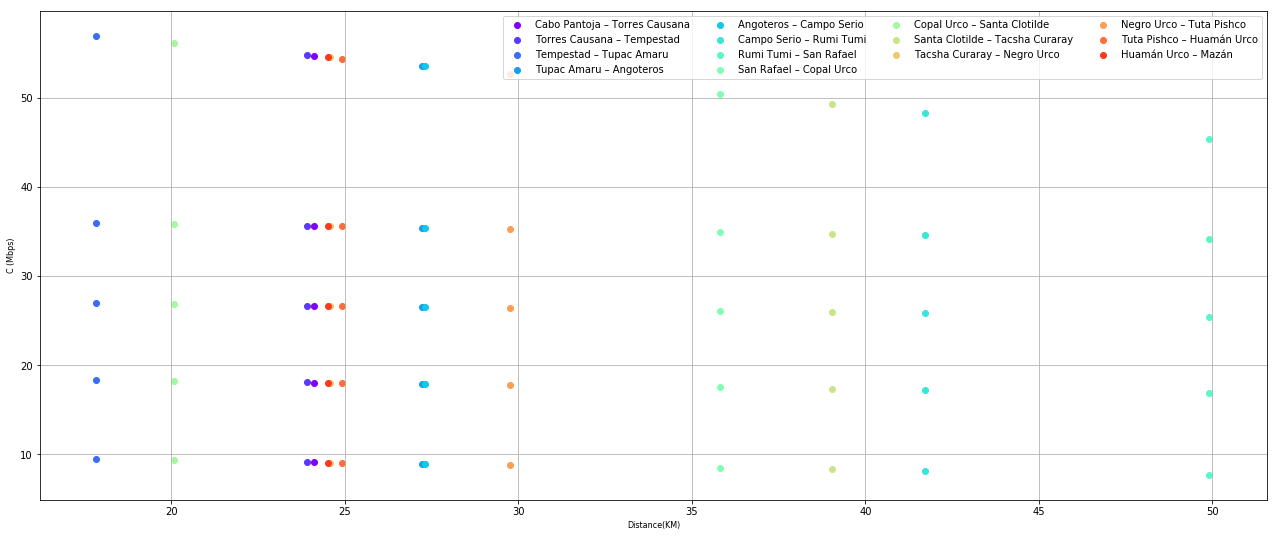
\includegraphics[width=0.7\textwidth]{img/valoresmbps.png}
		\caption{Capacidad del canal teórica respecto a la distancia para cada MCS con NV2}
		\label{valoresmbps}
	\end{figure}
	
	Los valores obtenidos y representados corresponden a las modulaciones comprendidas entre MCS8 y MCS12; no obstante, el interés de este estudio es determinar cual sería la modulación mínima utilizable de forma teórica en la red del Napo, asegurando así esa capacidad mínima definida de 44 Mbps por radioenlace. Como se ha comentado al inició del capítulo, y debido a la no disponibilidad de los valores relacionados con el \textit{throughput} para el protocolo NV2 y un ancho de banda de 40 Mhz, diseñaremos un sistema de coordenadas que relacione distancia y ancho de banda con el objetivo de aproximar los datos no conocidos respecto a 40 MHz en base a los conocidos de 20 Mhz.\\
	
	En conclusión a este análisis teórico y aproximación analítica, la Tabla \ref{table:capacidades} recoge los datos obtenidos, los cuales reflejan que para cumplir con los requesitos necesarios de la red cada radioenlace debe utilizar una modulación MCS10.   
	
\subsection{Estudio con RadioMobile}
	Una vez desarrolado el estudio teórico sobre la red, nuestro siguiente paso será realizar una representación simulada con el objetivo de obtener más información sobre la viabilidad de enlace relativa a los emplazamientos del proyecto. Para ello, utilizaremos los datos de geolocalización y distancia relacionados con los emplazamientos de la red del Napo los cuales se encuentran en las Tablas \ref{table:distancias} y \ref{table:geolocalizacion}, para introducirlos en la herramienta RadioMobile y crear así nuestra red simulada. Junto a la localización geográfica y altura de cada emplazamiento tendremos que configurar los principales parámetros de la red y de los equipos en la herramienta, esta combinación nos permitirá obtener una aproximación sobre la calidad del enlace en términos generales e individuales de la red. A continuación se detallan las características de los sistemas insertados en la herramienta para llevar a cabo la simulación:
	\begin{itemize}
		\item Potencia de transmisión: 32 dBm
		\item Sensibilidad en recepción: -96 dBm
		\item Pérdidas por cable: 1,5 dB
		\item Ganancia de antena: 30 dBm
		\item Tipo de antena: Omnidireccional
		\item Frecuencia: 5260 MHz
	\end{itemize}
	Una vez configurado los parámetros y características de los sistemas, obtenemos una representación simulada de la red tal y como se muestra en la Figura \ref{redNapo}. Dicha simulación está sujeta al modelo \textit{Longley-Rice} que utiliza la variabilidad de tiempo, posición y situación para realizar los cálculos respecto al balance de enlace.  
	\begin{figure}[H]
		\centering
		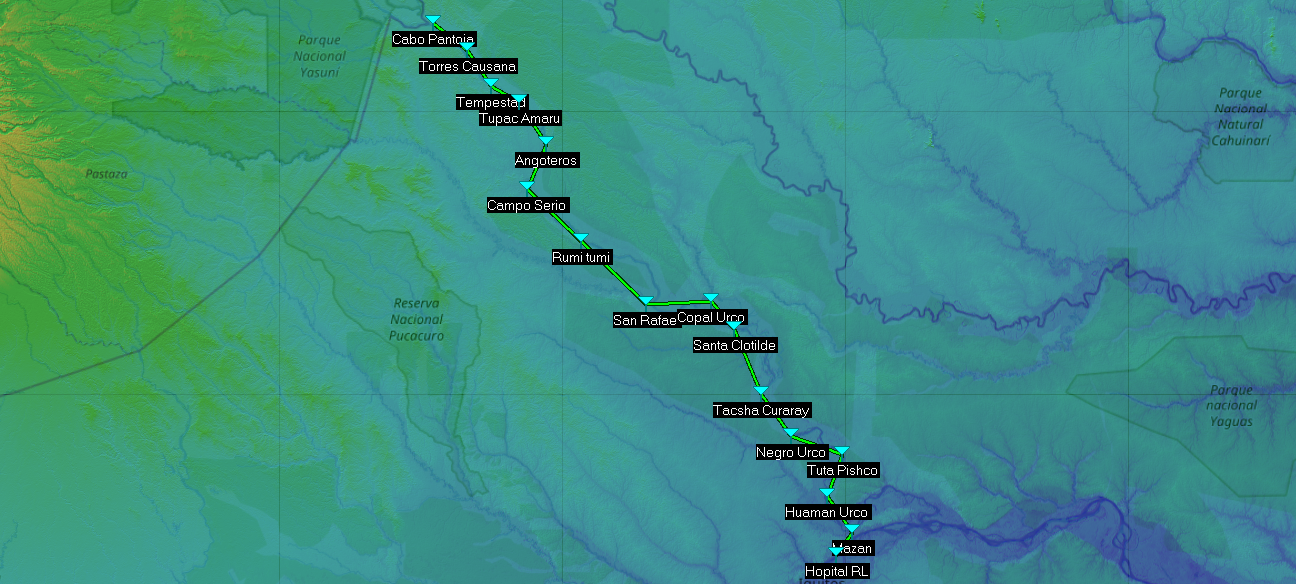
\includegraphics[width=0.7\textwidth]{img/redNapo.PNG}
		\caption{Representación de la red del Napo en RadioMobile.}
		\label{redNapo}
	\end{figure}
	La funcionalidad \textit{Radio Link} que se encuentra dentro de RadioMobile nos permite obtener una representación simulada del estado de cada radioenlace a través de la recreación del perfil geográfico y configuración de los sistemas involucrados en el enlace. Esto nos permite conocer los niveles de pérdidas, sensibilidad en recepción y margen dinámico de cada sistema de forma individual a través de la realización del balance de enlace. Dicho balance de enlace nos proporcionará información respecto a la sensibilidad y potencia en transmisión y recepción, para poder establecer la mínima tasa de transmisión soportada siempre y cuando cumpla con los requisitos de viabilidad de enlace mencionados al principio de este Trabajo Fin de Grado.\\\\
	
	Para poder obtener una tasa mínima que cumpla los requisitos de transmisión mínimos mencionados en el capítulo de introducción, debemos tener en cuenta el tipo de tecnología que estamos utilizando. En nuestro caso, las transmisiones pertenencientes a la nueva red del Napo se realizarán utilizando la tecnología \textit{Multiple Input Multiple Output}, junto al uso de NV2 como protocolo de acceso al medio. La utilización de MIMO hace que nos centremos en los valores pertenecientes a las MCS cuyos valores están comprendidos entre MCS8 y MCS15, dichas MCS a su vez están formadas desde una constelación BPSK (formada por dos símbolos) hasta una 64-QAM (formada por 64 símbolos). Para poder establecer una comparación entre la modulación adecuada por cada radioenlace tendremos que comparar la senbilidad en recepción de cada sistema obtenido mediante la simulación, con los valores típicos de sensibilidad para dichos MCS.\\
	
	Una vez expuesto el escenario y parametrización de la simulación, procedemos a realizar la misma con el objetivo de obtener la potencia recibida teórica en cada radioenlace y conocer así la viabilidad de los enlaces, los datos extraídos de esta simulación se encuentran en la Tabla \ref{table:rmEnlaceteorico}. La viabilidad de los enlaces vendrá marcado por la comparación entre le potencia teórica recibida y la sensibilidad existente para cada modulación utilizando en protocolo NV2, dichos datos se encuentran en la Tabla \ref{table:sensibilidadMCS}. A continuación, se detallan la conclusiones obtenidas del análisis simulado: 
	\begin{itemize}
		\item Existe línea de visión directa en la mayoría de casos, lo que implica asegurar la zona de Fresnel mínima para la viabilidad del enlace, en nuestro caso un sesenta por ciento.
		\item Habiendo analizado cada balance de enlace de forma individual, podemos realizar una extrapolación para el total de la red, asegurando así un margen dinámico que garantice la viabilidad del enlace. En el caso del diseño inicial dicho margen dinámico era de 20 dB, por tanto habiendo contrastado los datos obtenidos con la simulación no existe compromiso respecto a la viabilidad de enlace en cada punto de la red.
		\item En base al estudio análitico hecho, para asegurar la total funcionalidad de la red, habría que utilizar un MCS10 como mínimo para alcanzar una capacidad de enlace suficiente y necesaria.
	\end{itemize}
	
\subsection{Configuración de equipos}
Para poder recrear en laboratorio un escenario punto a punto de similares características a los de la red del Napo, utilizaremos dos equipos NetMetal 5 y dos portátiles con sistema operativo GNU/Linux. Los ordenadores portátiles actuarán de emisor y receptor en nuestra red local junto a los equipos NetMetal 5 que interconectarán dichos terminales finales entre sí, como se muestra en la Figura \ref{enlace}. Para obtener valores relacionados con los parámetros de QoS, se inyectará tráfico con la herramienta Iperf y Bandwidth test, utilizando uno de los portátiles como cliente y otro como servidor.\\\\

\begin{figure}[H]
	\centering
	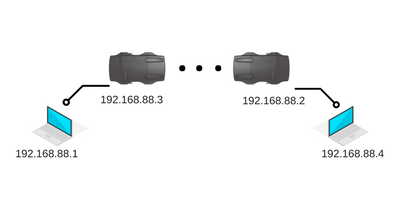
\includegraphics[width=0.7\textwidth]{img/escenario.png}
	\caption{Escenario de laboratorio punto a punto.}
	\label{enlace}
\end{figure}

Antes de comenzar a detallar cómo se ha realizado la configuración a nivel de laboratorio de los equipos, debemos apuntar que en nuestro caso las antenas utilizadas son dipolos elementales colocados en posición vertical y horizontal transmitiendo forma multimodal; en el caso del proyecto Napo cada radioenlace constará de una antena parabólica colocada en lo alto de una infraestructura metálica, cuya ganancia de transmisión está en torno a los 30 dB. \\

\section{Inyección de tráfico simulado}
Para conocer el rendimiento y prestaciones de los equipos realizaremos pruebas a nivel de red a través de la inyección de tráfico simulado. Para llevar a cabo dicha prueba, utilizaremos el software disponible para los sistemas operativos de distribución Linux Iperf y la herramienta de medida de ancho de banda proporcionada por MikroTik Bandwidth text, las cuales se detallan brevemente a continuación.\\

\subsection{Iperf}
Iperf \cite{Iperf} es una herramienta que permite realizar mediciones sobre el máximo rendimiento alcanzable respecto al ancho de banda y la calidad de un enlace red. Esto es posible mediante el análisis y recopilación de datos referentes a los protocolo de red TCP y UDP. Existe la variante Jperf, cuya única diferencia es la utilización de una interfaz gráfica en lugar de la entrada estándar de comandos.\\

La herramienta puede ser utilizada en modo cliente o en modo servidor, permitiendo realizar pruebas sobre la red hasta obtener los valores óptimos sobre la misma, tal y como se muestra en la Figura \ref{logTestIperf}.\\

Esto es gracias al ajuste y modificación de parámetros que permite la herramienta: según sea nuestro escenario y el objetivo de nuestras pruebas, podremos obtener un tipo específico de datos u otros. La elección de los parámetros de la herramienta será diferente según el protocolo de red (TCP o UDP) que utilicemos en cada caso. A continuación detallamos las posibilidades que ofrece en base a cada uno de ellos:\\

En primer lugar explicaremos los parámetros relacionados al protocolo UDP, el cual nos permite seleccionar un ancho de bando específico en nuestra comunicación y permite utilizar multidifusión si fuera necesario. Además, los datos reportados por la herramienta en este caso son los relacionados con la pérdida de paquetes, ya sea en cuantía o en porcentaje, y las medidas relacionadas con el jitter y retardo.\\

En segundo lugar, los parámetros configurables respecto a TCP están relacionados con la elección de un tamaño de ventana TCP fijo para la comunicación, otorgando datos respecto al ancho de banda medido en la comunicación y el tamaño MSS/MTU.

\begin{figure}[H]
	\centering
	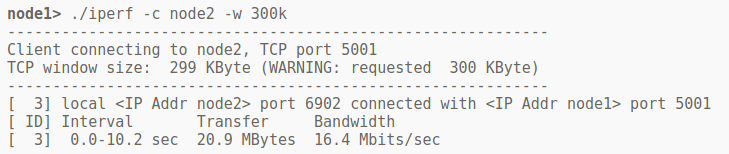
\includegraphics[width=0.7\textwidth]{img/log_iperf.png}
	\caption{Log obtenido al realizar una prueba con Iperf. Fuente: Iperf}
	\label{logTestIperf}
\end{figure}

\subsection{Bandwidth test}
\textit{Bandwidth test} es la herramienta desarrollada por el fabricante que nos permite realizar medidas entre equipos MikroTik en lo que a \textit{throughput} se refiere. Dicha herramienta está disponible tanto para la interfaz web, cómo para la consola.\\

Para llevar a cabo dicho test, debemos configurar uno de los routers que forman la red en modo servidor, y el resto en modo cliente, además la herramienta nos proporciona una serie de parámeotros configurables respecto a la red activa tales cómo: dirección, duración, tamaño de paquete, etc... \\
En función de estos parámetros el resultado de la prueba será de un modo u otro, y nos proporcionará los valores deseados respecto a el número de paquetes pérdidos, velocidades medias y totales en recepción y transmisión de la conexión activa. A continuación, en la Figura \ref{logTest} se muestra un ejemplo del log obtenido al realizar una prueba utilizando la herramienta mencionada anteriormente.

\begin{figure}[H]
	\centering
	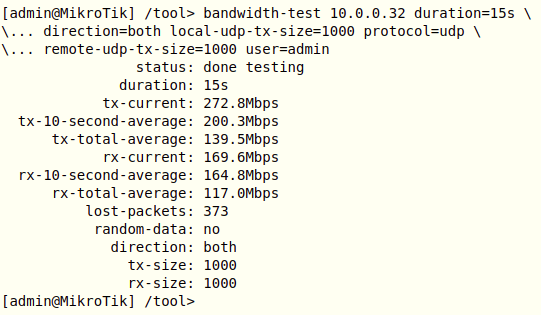
\includegraphics[width=0.7\textwidth]{img/log_test.png}
	\caption{Log obtenido al realizar una prueba sobre un enlace MikroTik activo. Fuente: Mikrotik Router and Wireless}
	\label{logTest}
\end{figure}

\section{Monitorización y gestión: Zabbix}
En esta sección se explicará la integración llevada a cabo con el escenario configurado en laboratorio y el \textit{software} de monitorización Zabbix. Así mismo, se procederá a explicar de manera más detallada el funcionamiento de la herramienta seleccionada en el marco contextual definido al inicio de este Trabajo Fin de Grado.\\

Antes de realizar la configuración del escenario formado en laboratorio, se procede a explicar cómo se va a llevar a cabo la integración de Zabbix y dicho escenario. Esto se llevará a cabo mediante el uso de plantillas XML y el protocolo SNMP, el cual nos permite intercambiar información entre los dispositivos involucrados.\\
 
El protocolo SNMP (\textit{Simple Network Management Protocol}) es un protocolo que corresponde con la capa de aplicación y facilita el intercambio de información administrativa entre los dispositivos que componen una red, ya sean \textit{routers}, \textit{switches}, etc... Este protocolo facilita a los administradores de red conocer en todo momento el estado de la red, así cómo la posibilidad de interactuar con la misma tomando acciones de prevención, resolución de problemas y estudio sobre escalabilidad.\\

Para lograr esto, SNMP accede a la MIB (\textit{Management Information Base}) de los equipos. La MIB es una colección de información referente al equipo organizada de forma jerárquica mediante un árbol, para llevar a cabo una eficiente búsqueda y consulta de los objetos que se encuentran dentro del árbol, se organizan en subconjuntos denominados organizaciones.\\\\

Cada objeto, denominado OID (\textit{Object Identifier}) contiene un valor asociado al parámetro que representa, ya sea en formato de cadena de carácteres o en formato numérico, para conseguir dicho valor se ha de realizar una búsqueda descendente del árbol que forma la MIB, ya sea bien utilizando la nomenclatura numérica que tiene cada organización seguida de un punto (1.3.6....) o bien utilizando el nombre de cada organización seguido de un punto (iso.identified....). Ambos métodos permiten recuperar el valor del parámetro deseado y utilizarlo en nuestra integración.\\

Así mismo, el funcionamiento de SNMP involucra a los siguiente agentes:

\begin{itemize}
	\item Sistema administrador: Capaz de ejecutar aplicaciones (comandos) capaces de controlar los dispositivos involucrados en la red, proporcionando métricas útiles para el administrador en cuánto a los recursos del equipo.
	\item Dispositivo administrado: Equipo que contiene el agente SNMP y forma parte de la red recogiendo información usando el protocolo SNMP.
	\item Agente SNMP: Permite realizar una administración de la forma otorgada por el equipo de manera local y jerarquizarlo en forma de árbol y en un formato compatible al intercambio de información usando dicho protocolo.
\end{itemize}

SNMP no sólo nos permite recorrer el árbol MIB y obtener información de los equipos, sino que mediante aplicaciones (comandos), es posible realizar simples operaciones sobre la estructura jerarquizada de los equipos, dichos comando se describen a continuación:

\begin{itemize}
	\item Lectura/Escritura: Permiten al administrador leer/modificar los valores de las variables almacenados dentro de los dispositivos.
	\item Notificación: Permite a los equipos reportar eventos de manera asíncrona al administrador. 
	\item Transversales: Permiten a los equipos recolectar información de los elementos cercanos en la red y conformar tablas relacionadas a la información obtenida. 
\end{itemize}

\subsection{Integración de escenario}
Una vez explicado todo lo que implica el uso de SNMP y la jerarquización de los objetos existente en los equipos y cómo es posible realizar consultas a dichos objetos, procedemos a explicar cómo se va a integrar la información procedente de los equipos con Zabbix. Una de las facilidades que nos ofrece la herramienta es que podemos crear \textit{items} tal y como se muestra en la Figura \ref{xmlTest}, aprovechando la información que nos proporcionan los OIDs en función de los parámetros que deseemos monitorizar. Para ello deberemos seguir el estándar XML, utilizando una plantilla como la mencionada antes e importarla en el sistema. De igual forma que podemos importar datos, existe la posibilidad de exportarlos, ofreciendo así versatilidad a la hora de integrar cualquier equipo en un sistema diferente. En el marco del proyecto los principales parámetros de interés son los referentes a salud de los equipos (carga CPU, temperatura, etc...) y a tráfico obtenido. 

\begin{figure}[H]
	\centering
	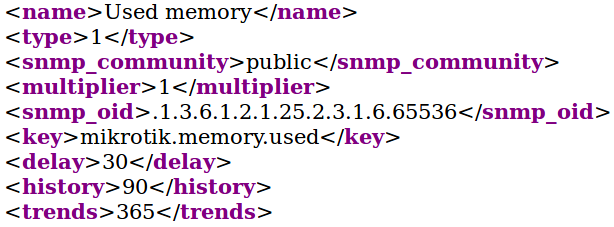
\includegraphics[width=0.7\textwidth]{img/xml_example.png}
	\caption{Ejemplo de configuración de un item sobre XML en Zabbix}
	\label{xmlTest}
\end{figure}

Una vez cargados los dispositivos involucrados en la plataforma, Zabbix ofrece varias herramientas para realizar un seguimiento sobre dichos elementos y otorgar control total sobre ellos al administrador, como por ejemplo configurando \textit{dashboards} de seguimiento, alertas sobre equipos, creación de mapas de redes, etc. A continuación se procede a detallar algunas de las aplicaciones utilizadas en este Trabajo Fin de Grado cuyo objetivo es monitorizar y obtener un control total de la red:\\

En primer lugar, nos hemos centrado en la representación gráfica del rendimiento que otorgan los equipos a nivel de red, para ello, hemos utilizado la aplicación que ofrece la propia herramienta que permite realizar gráficas a nivel de interfaz, como se muestra en la Figura \ref{zabbixMeasure}, una aplicación interesante de estas gráficas es que se puede realizar un tablero configurable conjunto, es decir, integrar dicha gráfica (o similares) de diferentes dispositivos en un único tablero, otorgando así al administrador una visión global del tráfico entrante y saliente de la red en conjunto.

\begin{figure}[H]
	\centering
	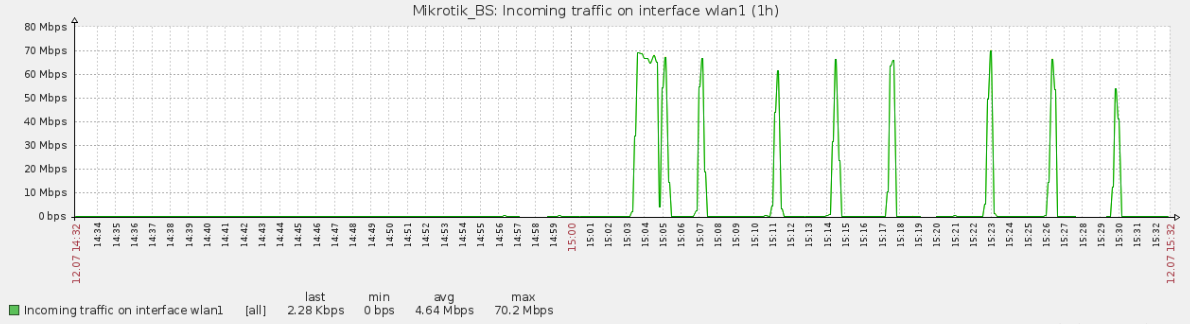
\includegraphics[width=0.7\textwidth]{img/zabbix_measure.png}
	\caption{Ejemplo de representación gráfica de tráfico mostrado en un Dashboard de Zabbix.}
	\label{zabbixMeasure}
\end{figure}

En segundo lugar, Zabbix ofrece alertas configurables en función de los \textit{items} cargados en la plantilla XML tal y como se muetra en la Figura \ref{zabbixResume}; esto quiere decir que la herramienta ofrece \textit{triggers} configurables, ya sea bien de forma predeterminada o personalizada, que permiten establecer valores umbral para los diferentes niveles de alerta que ofrece la herramienta, generando así una categorización de problemas y otorgando al administrador una versión prioritaria de la acción que ha de ser tomada. Las alertas no son configuradas únicamente si el programa se está ejecutando en primer plano, Zabbix ofrece una extensión llamada PostFix \cite{PostFix} que permite integrar y configurar alertas para que sean enviadas mediante email.\\
De igual forma, Zabbix mantiene un archivo histórico de logs el cual otorga cierta ventaja a la hora de actuar al administrador, ya sea en labores de mantemiento de la red o bien en labores predictivas. 

\begin{figure}[H]
	\centering
	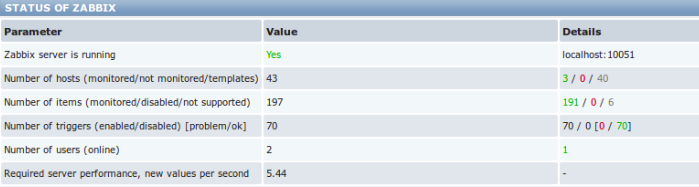
\includegraphics[width=0.7\textwidth]{img/zabbix_resume.png}
	\caption{Ejemplo del estado de la red en Zabbix}
	\label{zabbixResume}
\end{figure}

Por último, otra aplicación interesante en el marco del proyecto es la creación de mapas de red, como muestra la Figura \ref{zabbixNetwork}, la cual permite al administrador no sólo jerarquizar los equipos en función de nombres o por IPs, si no que otorga la posibilidad de subdividir una red total en subredes de forma que puedan aislarse cada una de ellas en subconjuntos, consiguiendo así un análisis más rápido y eficaz que si tuviera que realizarse de toda la red en conjunto. Aparte de esto, subdividir las redes porporciona la capacidad de asignar cada subred a un grupo de técnicos determinado evitando así que la gestión de una única subred involucre al resto de la misma.

\begin{figure}[H]
	\centering
	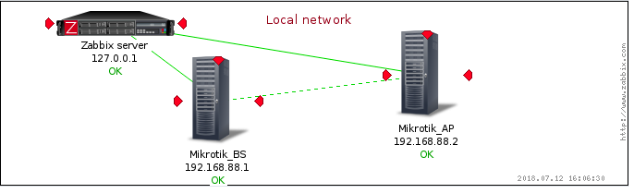
\includegraphics[width=0.7\textwidth]{img/zabbix_networks.png}
	\caption{Ejemplo de jerarquización de redes en Zabbix}
	\label{zabbixNetwork}
\end{figure}

En definitiva y reuniendo todo lo explicado a lo largo de este capítulo, Zabbix no sólo es una solución que cumple con los requisitos mínimos de monitorización de redes requeridos en el proyecto, si no que su amplia variedad de integraciones y aplicaciones.Zabbix no sólo permite una fácil integración con los dispositivos físicos mediante el uso de plantilla XML y protocolo SNMP, si no que también ofrece una solución a todo lo referido con \textit{software} de terceros. Todo esto a partir de la editabilidad de la mayor parte su funcionalidad básica para hacer que el administrador de redes tenga la mayor cantidad de información sobre los equipos, concentrada de tal forma que su actuación se inminente y precisa si esta fuera requerida.
	\chapter{Resultados obtenidos en las medidas de prestaciones}
\label{cap:resultaldos_obtenidos}

En este capítulo se expondrán los datos y conclusiones obtenidos durante la realización de medidas de prestaciones realizadas sobre los equipos seleccionados en este Trabajo de Fin de Grado. Para llevar a cabo el desarrollo de este capítulo, no sólo se ha tenido en cuenta los resultados y pruebas realizados en entornos simulados, sino que también los aportados por la PUCP de sus configuraciones y de las medidas realizadas en campo tras la instalación en el entorno real del río Napo.\\

Por un lado se expondrán los datos obtenidos en el entorno simulado, es decir utilizaremos la configuración y herramientas mencionadas en el Capítulo \ref{cap:metodologia} para realizar las pruebas respecto a la tasa de transmisión y recepción de los equipos. De foma complementaria se utilizará la herramienta RadioMobile para obtener una representación de la red obteniendo una estimación del balance de enlace de la red.\\

Por otro lado se recogerán los valores proporcionados por la PUCP durante la realización de pruebas y se contrastarán con las medidas obtenidas en laboratorio. Cabe destacar que las pruebas mencionadas sólo han podido realizarse en un conjunto de radioenlaces determinados. Dichos enlaces son los comprendidos entre Santa Clotilde e Iquitos.\\

Por último y como objetivo final de este capítulo, se tratará de explicar ambos conjuntos de datos para así poder realizar un análisis del estado de cada radioenlace perteneciente a la red del Napo, teniendo en cuenta el objetivo explicado en el capítulo \ref{cap:introduccion}.
 
\section{Análisis de resultados}
Para llevar a cabo el desarrollo y análisis de los resultados hemos tomado como configuración referencia los valores proporcionados por la PUCP, los cuales se detallan a continuación:
\begin{itemize}
	\item Tiempo de la observación: 25 segundos.
	\item Modulación empleada: MCS10
	\item Frecuencia: 5805 Hz
	\item Estándar: 802.11n
	\item Ancho de banda: 40 MHz
\end{itemize}
De igual forma se ha utilizado la herramienta propuesta por la PUCP, que en este caso es la propietaria de MikroTik descrita en el capítulo \ref{cap:metodologia}; aunque en laboratorio resulta más interesante el empleo de herramientas de inyección de tráfico independientes del producto, en la instalación en campo es enormemente más sencillo emplear las herramientas embebidas en los sistemas de comunicaciones, y conviene utilizar la misma herramienta para las mediciones en campo y en laboratorio para que los resultados de éstas sean plenamente comparables. Para llevar a cabo las pruebas respecto a la capacidad de cada radioenlace  utilizaremos el siguiente comando en la terminal de los equipos, que está compuesto por los siguientes parámetros: dirección destino, sentido de la comunicación y tiempo de observación:
\begin{lstlisting}
 tool bandwidth-test xx.xx.xx.xx direction=both duration=25
\end{lstlisting}

Una vez concretado los parámetros y configuraciones base de las pruebas que vamos a realizar, es necesario conocer los valores que se han obtenido en las pruebas de campo y contrastarlos con los valores teóricos que hemos obtenido con la simulación. En este caso aparte de los valores respecto a la capacidad del enlace, es importante conocer la potencia en recepción que está recibiendo cada radioenlace y analizar si dichos valores carecen o no de sentido. Por tanto, en primer lugar haremos un primer análisis tomando como referencia los datos obtenidos en simulación y en campo respecto a la potencia de señal recibida y en segunda lugar realizaremos un análisis similar, salvo que en este caso el objeto de análisis será la capacidad del enlace.\\

Para poder realizar una comparación coherente entre los datos aportados utilizaremos, por un lado los datos teóricos respecto a la sensibilidad mínima necesaria para cada modulación utilizando el protocolo NV2, tal y como se muestra en la Tabla \ref{table:sensibilidadMCS}. Y por otro lado, los datos obtenidos de la simulación hecha con RadioMobile y los valores proporcionados por los equipos durante la realización de pruebas, que se muestran en la Tabla \ref{table:sensibilidadCampoObtenida}.\\
En este caso nos interesa centrarnos en el valor correspondiente a la modulación MCS10 ya que es la cual ha sido utilizada para realizar pruebas. Dicha modulación tiene una sensibilidad mínima de -90 dBm, por tanto para asegurar un correcto rendimiento del enlace utilizando esa modulación cada radioenlace debe estar por encima de dicho valor. Cómo vemos, para los valores teóricos y empíricos de los radioenlaces comprendidos entre Cabo Pantoja e Iquitos se cumple, por tanto podemos utilizar la modulación MCS10 para transmitir.\\

De igual forma los valores simulados han sido obtenidos teniendo en cuenta los parámetros tiempo y situaciones que ofrece RadioMobile, los cuales son editables y en este caso han sido fijados con valores de 99\% y 80\%, respectivamente. La edición de estos parámetros implica una variación en los niveles de señal medio afectando de manera directa en las condiciones estadísticas que definen al modelo. En resumen, esto se traduce a que durante el 80\% del tiempo la atenuación no excederá el valor que obtengamos, al menos, un 99\% del tiempo.\\

En conclusión, observamos como para una distancia cercana a los 30 Km existe una medida anómala, esta medidas es la obtenida en el enlace de Negro Urco - Tuta pishco ya que los datos experimentales obtenidos distan mucho de los teóricos. Aunque se sobrepase el límite de -90 dBm que marca la modulación MCS10 se debería corregir o hacer un reajuste a ese radioenlace puesto que puede poner en compromiso el rendimiento total de la red.\\

A continuación para completar el análisis realizaremos un procedimiento similar al anterior pero teniendo en cuenta los valores obtenidos en las pruebas realizadas frente a la capacidad de cada enlace. En este análisis serán utilizados los valores obtenidos en el entorno de laboratorio y los proporcionados por la PUCP, los cuales se recogen en las Tablas \ref{table:medidasInstLabNapo}, \ref{table:medidasMediasLabNapo}, \ref{table:medidasInstNapo} y \ref{table:medidasMediasNapo} respectivamente. \\

En resumen, y analizando el conjunto de las pruebas realizadas y aportadas por la PUCP se destaca lo siguiente:

\begin{itemize}
	\item El enlace de Santa Clotilde - Tacsha Curaray no sólo obtiene mejores tasas pese a ser uno de los más largos, sino que también obtiene una mayor potencia de señal recibida que los enlaces que son más cortos. Esto pone en duda la corrección de la instalación en los otros enlaces cuya distancia es aproximadamente la mitad y consiguen unas tasas bastante inferiores. En este caso, debería revisarse la configuración de los equipos y las instalaciones para conocer el motivo de dichos datos. 
	
	\item El enlace Tacsha Curaray - Negro Urco también es llamativo. Siendo un enlace cuya distancia es intermedia, en torno a 25 Km, obtiene unos valores de señal recibida y tasa muy altos en comparación. La explicación a esto podría deberse a las reflexiones de los elementos geológicos existentes entre el enlace, aunque es llamativa esa diferencia tan remarcada de potencia de señal recibida entre los enlaces de una distancia similar.
	
	\item El enlace Negro Urco - Tuta Pishco siendo un enlace cercano a los 30 km, es decir no siendo un enlace excesivamente largo, obtiene una tasa muy inferior a la esperada aunque su señal de potencia recibida sea la más baja de todos los enlaces analizados. En similares condiciones, enlaces con las mismas características obtienen un rendimiento mucho mejor que este, de tal forma que existe un problema en este enlace, bien sea de configuración de equipos o de apuntamiento de antenas.
	
	\item Respecto a los valores obtenidos en laboratorio y los posibles alcanzados en el escenario real del proyecto, el rendimiento de los equipos \textit{MikroTik} podría asegurar los objetivos definidos en el capítulo \ref{cap:introduccion} de poder mantener la cohesión de las dos redes. 
\end{itemize}

	\chapter{Conclusiones}
\label{cap:conclusion}

\section{Competencias adquiridas}
Para el desarrollo de este Trabajo Fin de Grado he aplicado todos los conocimientos y competencias adquiridos durante la carrera a nivel de configuración de redes, análisis y diseño de escenarios simulados mediante el uso \textit{RadioMobile}, desarollo de código a bajo nivel y alto, utilizando en este último librerías para la extracción, procesado y representación de datos. Por consiguiente cómo objetivo de máximo interés, el haber aplicado todas estás tecnologías y competencias sobre un escenario real tanto cómo es el proyecto Napo y sobre los equipos NetMetal 5, realizando un estudio sobre el la red en conjunto y extraer conclusiones frente a la viabilidad y rendimiento de los equipos tratando de cumplir siempre con los objetivos del proyecto Napo.\\\\

Realizar este Trabajo Fin de Grado me ha aportado conocimientos generales en cuánto al diseño y despliegue de redes en países subdesarrollados. De igual forma, destacaría la capacidad de gestión y coordinación con los compañeros de la PUCP, los cuáles han formado parte activa durante desarrollo de este Trabajo Fin de Grado aportando datos y realizando pruebas de campo, para que la labor de diseño, análisis de pruebas y extracción de resultados sea lo más exacta posible. \\\\

Por último y como competencia clave, destacaría el poder trabajar con equipos reales a nivel de laboratorio, realizar pruebas a nivel de red, integrar los equipos con un \textit{software} de monitorización y en base a todo ello, extraer conclusiones y aportar valor desde un plano simulado en laboratorio sobre el rendimiento de los equipos en el escenario del proyecto Napo .

\section{Trabajos futuros}
En primer lugar y analizando el rendimiento ofrecido por lo equipos a nivel de laboratorio, sería interesante tratar de replicar el tráfico existente en las dos redes, tanto la de datos cómo la de telemedicina, realizando túneles MPLS para su diferenciación y agregación. De igual forma, se trataría de integrar la funcionalidad de esta red principal compuesta por los dipositivos NetMetal 5 con los nodos, cuya placa integrada es Alix, asociado a la creación de una red de \textit{backup}.\\\\

En segundo lugar, para conseguir una reproducción y extracción de valores más parejos frente al contexto del proyecto, deberían realizarse no sólo pruebas a nivel de laboratorio, si no que también dichas pruebas deberían ser realizadas con las distancias existentes en cada radioenlace del proyecto obteniendo así una reproducción más exacta en cuánto al rendimiento de los equipos.\\\\

Por último, realizar una integración con Zabbix del sistema de la red conjunto, teniendo en cuenta todos los dispositivos que están involucrados en la red y realizar una perfecta jerarquización de la misma. No sólo a la hora de integrar todo lo relacionado con alertas pudiendo crear asignaciones en función de las subredes existentes. De igual modo utilizar la aplicación que utiliza Zabbix respecto al \textit{discovery} para generar una base de datos representativa con todos los elementos que componen la red.
	\chapter{Anexos}
\label{cap:anexo}
\section{Tablas empleadas}

\begin{table}[H]
	\begin{center}
		\begin{tabular}{|l|l|}
			\hline
			Enlaces Backhaul & Tráfico total (Kbps) \\
			\hline 
			Cabo Patonja - Torres Causana & 44528 \\ \hline
			Torres Causana – Tempestad & 44956 \\ \hline
			Tempestad – Tupac Amaru & 41572 \\ \hline
			Tupac Amaru – Angoteros & 39344 \\ \hline
			Angoteros – Campo Serio  & 37804 \\ \hline
			Campo Serio – Rumi Tuni & 35108 \\ \hline
			Rumi Tuni -  San Rafael & 33012 \\ \hline
			San Rafael – Copal Urco & 28604 \\ \hline
			Copal Urco – Santa Clotilde & 26112 \\ \hline
			Santa Clotilde – Tacsha Curaray & 24228 \\ \hline
			Tacsha Curaray – Negro Urco & 20044 \\ \hline
			Negro Urco – Tuta Pischo & 19316 \\ \hline
			Tuta Pishco – Huaman Urco & 12464 \\ \hline
			Huamán Urco – Mazán & 11260 \\ \hline
			Mazán – Iquitos & 5696 \\ \hline
			
		\end{tabular}
	\end{center}
	\caption{Tráfico total por enlace}
	\label{table:RLPUCP}
\end{table}

\begin{table}[H]
	\begin{center}
		\begin{tabular}{|l|l|l|}
			\hline
			Enlaces Backhaul & Latitud & Longitud\\
			\hline 
			Cabo Patonja & $^{\circ}$0 '58 "12,80 S & $^{\circ}$75 '10 "30,10 O  \\ \hline
			Torres Causana & $^{\circ}$1 '6 "15,40 S & $^{\circ}$75 '0 "15,80 O \\ \hline
			Tempestad & $^{\circ}$1 '16 "57,70 S & $^{\circ}$74 '53 "2,30 O \\ \hline
			Tupac Amaru & $^{\circ}$1 '21 "47,00 S & $^{\circ}$74 '44 "42,00 O \\ \hline
			Angoteros & $^{\circ}$1 '34 "6,80 S & $^{\circ}$74 '36 "40,60 O \\ \hline
			Campo Serio & $^{\circ}$1 '47 "40,80 S & $^{\circ}$74 '42 "28,60 O \\ \hline
			Rumi Tumi & $^{\circ}$2 '3 "14,00 S & $^{\circ}$74 '26 "10,50 O \\ \hline
			San Rafael & $^{\circ}$2 '21 "53,80 S & $^{\circ}$74 '6 "44,10 O \\ \hline
			Copal Urco & $^{\circ}$2 '20 "52,10 S & $^{\circ}$73 '47 "24,70 O \\ \hline
			Santa Clotilde & $^{\circ}$2 '29 "22,40 S & $^{\circ}$73 '40 "40,70 O \\ \hline
			Tacsha Curaray & $^{\circ}$2 '48 "47,60 S & $^{\circ}$73 '32 "27,20 O \\ \hline
			Negro Urco & $^{\circ}$3 '1 "23,10 S & $^{\circ}$73 '23 "31,50 O \\ \hline
			Tuta Pishco & $^{\circ}$3 '6 "31,40 S & $^{\circ}$73 '8 "17,50 O \\ \hline
			Huamán Urco & $^{\circ}$3 '19 "7,60 S & $^{\circ}$73 '13 "1,90 O \\ \hline
			Mazán & $^{\circ}$3 '29 "59,90 S & $^{\circ}$73 '5 "28,00 O \\ \hline
			Hospital Regional de Loreto & $^{\circ}$3 '36 "46,86 S & $^{\circ}$73 '10 "20,05 O \\ \hline
		\end{tabular}
	\end{center}
	\caption{Geolocación de los emplazamientos del NAPO}
	\label{table:geolocalizacion}
\end{table}

\begin{table}[H]	
	\begin{center}
		\begin{tabular}{|l|l|l|}
			\hline
			Enlace & Altura torres & Distancia \\
			\hline 
			Cabo Pantoja – Torres Causana & 45 m – 45 m & 24,11 Km \\ \hline	
			Torres Causana – Tempestad & 45 m – 60 m & 23,92 Km \\ \hline
			Tempestad – Tupac Amaru & 60 m – 45 m & 17,84 Km \\ \hline
			Tupac Amaru – Angoteros & 45 m – 66 m & 27,24 Km \\ \hline
			Angoteros – Campo Serio & 66 m – 66 m & 27,32 Km \\ \hline
			Campo Serio – Rumi Tumi & 66 m – 90 m & 41,72 Km \\ \hline
			Rumi Tumi – San Rafael & 90 m – 90 m & 49,89 Km \\ \hline
			San Rafael – Copal Urco & 90 m – 54 m & 35,82 Km \\ \hline
			Copal Urco – Santa Clotilde & 54 m – 72 m & 20,09 Km \\ \hline
			Santa Clotilde – Tacsha Curaray & 72 m – 72 m & 39,05 Km \\ \hline
			Tacsha Curaray – Negro Urco & 72 m – 75 m & 24,58 Km \\ \hline
			Negro Urco – Tuta Pishco & 75 m- 57 m & 29,75 Km \\ \hline
			Tuta Pishco – Huamán Urco & 57 m – 66 m & 24,93 Km \\ \hline
			Huamán Urco – Mazán & 66 m – 69 m & 24,52 Km \\ \hline
			Mazán - Hospital Regional Loreto & 69 m - 30 m & 15,45 Km \\ \hline
		\end{tabular}
	\end{center}
	\caption{Altura de torres y distancia entre emplazamientos del NAPO}
	\label{table:distancias}
\end{table}

\begin{table}[H]
	\begin{center}
		\begin{tabular}{|l|l|l|}
			\hline
			Enlace & Mbps obtenida & Distancia \\
			\hline 
			Cabo Pantoja – Torres Causana & 53,34973333333333 & 24,11 Km \\ \hline	
			Torres Causana – Tempestad & 53,367466666666665 & 23,92 Km \\ \hline
			Tempestad – Tupac Amaru & 53,93493333333333 & 17,84 Km \\ \hline
			Tupac Amaru – Angoteros & 53,0576 & 27,24 Km \\ \hline
			Angoteros – Campo Serio & 53,05013333333333 & 27,32 Km \\ \hline
			Campo Serio – Rumi Tumi & 51,70613333333333 & 41,72 Km \\ \hline
			Rumi Tumi – San Rafael & 50,943599999999996 & 49,89 Km \\ \hline
			San Rafael – Copal Urco & 52,2568 & 35,82 Km \\ \hline
			Copal Urco – Santa Clotilde & 53,72493333333333 & 20,09 Km \\ \hline
			Santa Clotilde – Tacsha Curaray & 51,95533333333333 & 39,05 Km \\ \hline
			Tacsha Curaray – Negro Urco & 53,30586666666667 & 24,58 Km \\ \hline
			Negro Urco – Tuta Pishco & 52,82333333333333 & 29,75 Km \\ \hline
			Tuta Pishco – Huamán Urco & 53,273199999999996 & 24,93 Km \\ \hline
			Huamán Urco – Mazán & 53,31146666666667 & 24,52 Km \\ \hline
			Mazán - Hospital Regional Loreto & 54,158 & 15,45 Km \\ \hline
		\end{tabular}
	\end{center}
	\caption{Valores de capacidad teórica respecto a cada radioenlace utilizando una MCS10 para NV2 y 40 Mhz}
	\label{table:capacidades}
\end{table}

\begin{table}[H]
	\begin{center}
		\begin{tabular}{|l|l|l|l|}
			\hline
			Enlace & Tráfico Tx (Mbps) & Tráfico Rx (Mbps) & Tráfico total (Mbps) \\
			\hline 
			Santa Clotilde – Tacsha Curaray & 49,5 & 33,7 & 83,2  \\ \hline
			Tacsha Curaray – Negro Urco & 55,8 & 61,3 & 117,1 \\ \hline
			Negro Urco – Tuta Pishco & 13,3 & 4,7 & 18 \\ \hline
			Tuta Pishco – Huamán Urco & 29,7 & 43,8 & 73,5 \\ \hline
			Huamán Urco – Mazán & 33,7 & 28,8 & 62,5 \\ \hline
			Mazán - Iquitos & 41,3 & 50,8 & 92,1 \\ \hline
		\end{tabular}
	\end{center}
	\caption{Valores instántaneos obtenidos en campo }
	\label{table:medidasInstNapo}
\end{table}

\begin{table}[H]
	\begin{center}
		\begin{tabular}{|l|l|l|l|}
			\hline
			Enlace & Tráfico Tx (Mbps) & Tráfico Rx (Mbps) & Tráfico total (Mbps)\\
			\hline 
			Santa Clotilde – Tacsha Curaray & 67,6 & 56,3 & 123,9\\ \hline
			Tacsha Curaray – Negro Urco & 48,6 & 51,5 & 100,1 \\ \hline
			Negro Urco – Tuta Pishco & 6,4 & 3,7 & 10,1 \\ \hline
			Tuta Pishco – Huamán Urco & 32,5 & 36 & 68,5 \\ \hline
			Huamán Urco – Mazán & 30,3 & 25,6 & 55,9 \\ \hline
			Mazán - Iquitos & 30,6 & 43,5 & 74,1 \\ \hline
		\end{tabular}
	\end{center}
	\caption{Valores medios obtenidos en campo}
	\label{table:medidasMediasNapo}
\end{table}

\begin{table}[H]
	\begin{center}
		\begin{tabular}{|l|l|l|l|}
			\hline
			Enlace & Tráfico Tx (Mbps) & Tráfico Rx (Mbps) & Tráfico total (Mbps)\\
			\hline 
			Santa Clotilde – Tacsha Curaray & 71,2 & 66,2 & 137,4\\ \hline
			Tacsha Curaray – Negro Urco & 71,2 & 66,1 & 137,3 \\ \hline
			Negro Urco – Tuta Pishco & 71,3 & 66,3 & 137,6 \\ \hline
			Tuta Pishco – Huamán Urco & 71,6 & 67 & 138,6 \\ \hline
			Huamán Urco – Mazán & 69,6 & 66,2 & 135,8 \\ \hline
			Mazán - Iquitos & 71,2 & 67,1 & 138,3 \\ \hline
		\end{tabular}
	\end{center}
	\caption{Valores instántaneos obtenidos en Laboratorio}
	\label{table:medidasInstLabNapo}
\end{table}

\begin{table}[H]
	\begin{center}
		\begin{tabular}{|l|l|l|l|}
			\hline
			Enlace & Tráfico Tx (Mbps) & Tráfico Rx (Mbps) & Tráfico total (Mbps)\\
			\hline 
			Santa Clotilde – Tacsha Curaray & 57,4 & 47,2 & 104,6 \\ \hline
			Tacsha Curaray – Negro Urco & 55,5 & 46,5 & 102 \\ \hline
			Negro Urco – Tuta Pishco & 58 & 43,9 & 101,9 \\ \hline
			Tuta Pishco – Huamán Urco & 56,9 & 50,3 & 107,2 \\ \hline
			Huamán Urco – Mazán & 60,1 & 55,8 & 115,9 \\ \hline
			Mazán - Iquitos & 43,5 & 43,1 & 86,6 \\ \hline
		\end{tabular}
	\end{center}
	\caption{Valores medios obtenidos en laboratorio}
	\label{table:medidasMediasLabNapo}
\end{table}

\begin{table}[H]
	\begin{center}
		\begin{tabular}{|l|l|}
			\hline
			Modulación & Sensibilidad (dBm)\\
			\hline 
			MCS8 & -95 \\ \hline
			MCS9 & -93 \\ \hline
			MCS10 & -90 \\ \hline
			MCS11 & -87 \\ \hline
			MCS12 & -84 \\ \hline
			MCS13 & -79 \\ \hline
			MCS14 & -78 \\ \hline
			MCS15 & -75 \\ \hline
		\end{tabular}
	\end{center}
	\caption{Valores teóricos de sensibilidad para cada MCS utilizando el protocolo NV2}
	\label{table:sensibilidadMCS}
\end{table}


\begin{table}[H]
	\begin{center}
		\begin{tabular}{|l|l|l|}
			\hline
			Enlace & Potencia teórica (dBm) & Potencia práctica (dBm)\\
			\hline 
		Santa Clotilde – Tacsha Curaray & -78,1 & -67 \\ \hline
		Tacsha Curaray – Negro Urco & -54,5 & -45 \\ \hline
		Negro Urco – Tuta Pishco & -57,4 & -75  \\ \hline
		Tuta Pishco – Huamán Urco & -54,3 & -68 \\ \hline
		Huamán Urco – Mazán & -70,6 & -68 \\ \hline
		Mazán - Iquitos & -49,5 & -66 \\ \hline
		\end{tabular}
	\end{center}
	\caption{Potencia de señal obtenida según radioenlace de forma teórica y práctica}
	\label{table:sensibilidadCampoObtenida}
\end{table}

\begin{table}[H]
	\begin{center}
		\begin{tabular}{|l|l|l|}
			\hline
			 & NetMetal 5 & RM-MAX\\
			\hline 
		Máx. Consumo de potencia  & 23 W & 8 W \\ \hline
		Potencia de entrada & 8 - 30 VDC & 48 VDC \\ \hline
		Frecuencia de operación & 4920 - 6100 MHzs & 2,4 - 2,5 GHzs | 5125 - 5875 MHzs  \\ \hline
		MIMO & 3x3 & 2x2 \\ \hline
		Máx. Potencia de transmisión & 33 dBm & 23 dBm \\ \hline
		Ancho de canal & 20/40/80 MHzs & 5/10/20/40 MHzs \\ \hline
		Máx. \textit{Throughput} & 1300 Mbps & 50 Mbps \\ \hline
		\end{tabular}
	\end{center}
	\caption{Parámetros de los equipos NetMetal 5 y RM-MAX}
	\label{table:parámetrosEquipos}
\end{table}

\begin{table}[H]
	\begin{center}
		\begin{tabular}{|l|l|l|}
			\hline
			 & PowerBeam AC & AirFiber\\
			\hline 
		Máx. Consumo de potencia  & 8.5 W & 12 W \\ \hline
	    Rango de Frecuencias (MHzs)| PIRE Máx (dBm)  & 5150 - 5875 | 53 dBm & \makecell{5150 - 5250 | 49 dBm \\ 5250 - 5350 | 30 dBm \\ 5470 - 5725 | 30 dBm \\ 5725 - 5850 |36, 54 dBm } \\ \hline
	    
		Máx. Potencia de transmisión & 24 dBm & 26 dBm \\ \hline
		\end{tabular}
	\end{center}
	\caption{Parámetros de los equipos PowerBeam AC y AirFiber}
	\label{table:parámetrosEquiposUbiquiti}
\end{table}

\begin{table}[H]
	\begin{center}
		\begin{tabular}{|l|l|l|}
			\hline
			 & NetMetal 5 & RM-MAX\\
			\hline
            Ancho de canal & 20 - 40 MHzs & 20 - 40 MHzs\\
			\hline 
		Promedio pérdida paquete  & 12,68\% - 0,46\% & 46\% - 63,66\% \\ \hline
		Promedio retardo (ms) & 11,47 - 10,69 & 223,52 - 168,27 \\ \hline
		Promedio Bandwidth TCP (Mbps) & 10,12 - 19,30  & 1,44 - 0.005  \\ \hline
		Promedio Bandwidth UDP (Mbps) & 14,25 - 24,32  & 0,03 - 0.006  \\ \hline
		\end{tabular}
	\end{center}
	\caption{Resultados obtenidos al realizar pruebas sobre los equipos NetMetal 5 y RM-MAX}
	\label{table:pruebasEquipos}
\end{table}

\begin{table}[H]
	\begin{center}
		\begin{tabular}{|l|l|l|}
			\hline
			 & PowerBeam AC  & AirFiber 5x\\
			\hline
            Ancho de canal & 20 MHzs & 40 - 50 MHzs\\
			\hline 
		Promedio pérdida paquete  & 40\% & 20\% \\ \hline
		Promedio retardo (ms) & 183.07  & 10.31 \\ \hline
		Promedio Bandwidth TCP (Mbps) & 40  & 37 - 78 \\  \hline
		\end{tabular}
	\end{center}
	\caption{Resultados obtenidos al realizar pruebas sobre los equipos Ubiquiti}
	\label{table:pruebasEquiposUbiquiti}
\end{table}

\begin{table}[H]
	\begin{center}
		\begin{tabular}{|l|l|l|}
			\hline
			 &  0 Km  & 30 Km\\ \hline
            MCS8 & 10,4 & 8,8 \\ \hline 
		  MCS9 & 19,2 & 17,8 \\ \hline
		  MCS10 & 27,8 & 26,4 \\ \hline
		  MCS11 & 37 & 35,3 \\ \hline
		  MCS12 & 63,5 & 52,6 \\ \hline
		  MCS13 & 77,2 & - \\ \hline
		  MCS14 & 81,1 & - \\ \hline
		  MCS15 & 85,2 & - \\ \hline
		\end{tabular}
	\end{center}
	\caption{Valores respecto a \textit{throughput} (Mbps) obtenidos en expertimentos de campo utilizando el protocolo NV2}
	\label{table:pruebasNV2campo}
\end{table}

\begin{table}[H]
	\begin{center}
		\begin{tabular}{|l|l|l|}
			\hline
			 Emplazamiento (A - B)  & Lfs (dBm) & Prx (dBm)\\ \hline
            Cabo Pantoja - Torre Causana & 142,9 & -53,9 \\ \hline 
		   Torre Causana - Tempestad & 141,3 & -52,3 \\ \hline
		   Tempestad - Tupac Amaru & 139,1 & -50,1 \\ \hline
		   Tupac Amaru - Angoteros & 142,1 & -53,1 \\ \hline
		   Angoteros - Campo Serio & 146 & -57 \\ \hline
		   Campo Serio - Rumi Tumi & 146,6 & -57,6 \\ \hline
		   Rumi Tumi - San Rafael & 156,8 & -67,8 \\ \hline
		   San Rafael - Copal Urco & 146,2 & -57,2 \\ \hline
		   Copal Urco - Santa Clotilde & 139,6 & -50,6 \\ \hline
		   Santa Clotilde - Tacsha Curaray & 162,7 & -73,7 \\ \hline
		   Tacsha Curaray - Negro Urco & 156,6 & -67,6 \\ \hline
		   Negro Urco - Tuta Pishco & 153,3 & -64,3 \\ \hline
		   Tuta Pishco - Huamán Urco & 141,9 & -52,9 \\ \hline
		   Huamán Urco - Mazán & 151,1 & -62,1 \\ \hline
		   Mazán - Hospital Regional de Loreto & 137,8 & -48,8 \\ \hline
		\end{tabular}
	\end{center}
	\caption{Valores obtenidos mediante simulación con RadioMobile}
	\label{table:rmEnlaceteorico}
\end{table}

\section{Código utilizado}
El siguiente código es el utilizado para la representación de \textit{throughput} en función de la distancia  y MCS, guardado en el archivo \texttt{capacidades.py}:
\begin{lstlisting}[caption={Script utilizado para representar \textit{throughput} en función de la distancia.}\label{lst:script},captionpos=b][language=Python]
import csv
import pandas as pd
import math 
import numpy as np
import matplotlib.pyplot as plt
import matplotlib.cm as cm

dataset = pd.read_csv('localidades.csv', delimiter = ',')
dataset = pd.DataFrame(dataset)
dataset1 = pd.read_csv('medidas NV2 20Mhz.csv', delimiter=',')
dataset1 = pd.DataFrame(dataset1)
colors = cm.rainbow(np.linspace(0, 1, 15))
nombres_rl = dataset['Localidad (A-B)']
nombres_mcs = ['MCS8', 'MCS9', 'MCS10', 'MCS11', 'MCS12']
distances = dataset['Distancia (Km)']

distances_array = []
for d in distances:
d = float(d.replace(",","."))
distances_array.append(np.float(d))

coor_x1 = []
coor_x2 = []
coor_y1 = []
coor_y2 = []

dataset1 = dataset1[:5]
for x, y in zip(dataset1['0'], dataset1['30']):
coor_x1.append(0.0)
coor_y1.append(x.replace(",","."))
coor_x2.append(30.0)
coor_y2.append(y.replace(",","."))

coordenadas = [coor_x1, coor_y1, coor_x2, coor_y2]
coordenadas = np.transpose(coordenadas)

throughput_mods_20 = []

def throughput(fila,d):
return  ((np.float(d) - np.float(fila[0])) * (( (np.float(fila[3]))) - (( np.float(fila[1])))) / (np.float(fila[2])-np.float(fila[0])) + np.float(fila[1])*2)

for i in range(0, len(coordenadas)):
fila = coordenadas[i]
for d in range(0, len(distances_array)):
throughput_mods_20.append((throughput(fila, distances_array[d])))

throughput_rl_20 = np.reshape(throughput_mods_20, (5,15)).T

def printable(array):
print_var = []
for item in array:
print_var += [item]
return print_var

rl_mcs8 = throughput_rl_20[:,0]
rl_mcs9 = throughput_rl_20[:, 1]
rl_mcs10 = throughput_rl_20[:, 2]
rl_mcs11 = throughput_rl_20[:, 3]
rl_mcs12 = throughput_rl_20[:,4]

printable_mcs8 = printable(rl_mcs8)
printable_mcs9 = printable(rl_mcs9)
printable_mcs10 = printable(rl_mcs10)
printable_mcs11 = printable(rl_mcs11)
printable_mcs12 = printable(rl_mcs12)

fig, ax = plt.subplots(figsize=(22,9))
plt.xlabel('Distance(KM)', fontsize=8)
plt.ylabel('C (Mbps)', fontsize=8)

plt.plot(distances_array, printable_mcs8, '-', label=nombres_mcs[0])
plt.plot(distances_array, printable_mcs9, '-',  label=nombres_mcs[1])
plt.plot(distances_array, printable_mcs10, '-', label=nombres_mcs[2])
plt.plot(distances_array, printable_mcs11, '-', label=nombres_mcs[3])
plt.plot(distances_array, printable_mcs12, '-', label=nombres_mcs[4])

ax.legend(ncol=2)    
ax.grid(True)
plt.show()
fig.savefig('rectas.png', format='png', dpi=1000)

fig_1, ax = plt.subplots(figsize=(22,9))
plt.xlabel('Distance(KM)', fontsize=8)
plt.ylabel('C (Mbps)', fontsize=8)

for i, c in zip(range(0, 14), colors):
ax.scatter(distances_array[i], printable_mcs8[i], color=c, label=nombres_rl[i])
ax.scatter(distances_array[i], printable_mcs9[i], color=c)
ax.scatter(distances_array[i], printable_mcs10[i], color=c)
ax.scatter(distances_array[i], printable_mcs11[i], color=c)
ax.scatter(distances_array[i], printable_mcs12[i], color=c)

ax.legend(ncol=4)    
ax.grid(True)
plt.show()
fig_1.savefig('valoresmbps.png',format='png', dpi=1000)
\end{lstlisting}
	
	\bibliographystyle{acm}
	\bibliography{tfg}
	
\end{document}